\documentclass[twoside]{book}

% Packages required by doxygen
\usepackage{fixltx2e}
\usepackage{calc}
\usepackage{doxygen}
\usepackage[export]{adjustbox} % also loads graphicx
\usepackage{graphicx}
\usepackage[utf8]{inputenc}
\usepackage{makeidx}
\usepackage{multicol}
\usepackage{multirow}
\PassOptionsToPackage{warn}{textcomp}
\usepackage{textcomp}
\usepackage[nointegrals]{wasysym}
\usepackage[table]{xcolor}

% Font selection
\usepackage[T1]{fontenc}
\usepackage[scaled=.90]{helvet}
\usepackage{courier}
\usepackage{amssymb}
\usepackage{sectsty}
\renewcommand{\familydefault}{\sfdefault}
\allsectionsfont{%
  \fontseries{bc}\selectfont%
  \color{darkgray}%
}
\renewcommand{\DoxyLabelFont}{%
  \fontseries{bc}\selectfont%
  \color{darkgray}%
}
\newcommand{\+}{\discretionary{\mbox{\scriptsize$\hookleftarrow$}}{}{}}

% Page & text layout
\usepackage{geometry}
\geometry{%
  a4paper,%
  top=2.5cm,%
  bottom=2.5cm,%
  left=2.5cm,%
  right=2.5cm%
}
\tolerance=750
\hfuzz=15pt
\hbadness=750
\setlength{\emergencystretch}{15pt}
\setlength{\parindent}{0cm}
\setlength{\parskip}{3ex plus 2ex minus 2ex}
\makeatletter
\renewcommand{\paragraph}{%
  \@startsection{paragraph}{4}{0ex}{-1.0ex}{1.0ex}{%
    \normalfont\normalsize\bfseries\SS@parafont%
  }%
}
\renewcommand{\subparagraph}{%
  \@startsection{subparagraph}{5}{0ex}{-1.0ex}{1.0ex}{%
    \normalfont\normalsize\bfseries\SS@subparafont%
  }%
}
\makeatother

% Headers & footers
\usepackage{fancyhdr}
\pagestyle{fancyplain}
\fancyhead[LE]{\fancyplain{}{\bfseries\thepage}}
\fancyhead[CE]{\fancyplain{}{}}
\fancyhead[RE]{\fancyplain{}{\bfseries\leftmark}}
\fancyhead[LO]{\fancyplain{}{\bfseries\rightmark}}
\fancyhead[CO]{\fancyplain{}{}}
\fancyhead[RO]{\fancyplain{}{\bfseries\thepage}}
\fancyfoot[LE]{\fancyplain{}{}}
\fancyfoot[CE]{\fancyplain{}{}}
\fancyfoot[RE]{\fancyplain{}{\bfseries\scriptsize Generated by Doxygen }}
\fancyfoot[LO]{\fancyplain{}{\bfseries\scriptsize Generated by Doxygen }}
\fancyfoot[CO]{\fancyplain{}{}}
\fancyfoot[RO]{\fancyplain{}{}}
\renewcommand{\footrulewidth}{0.4pt}
\renewcommand{\chaptermark}[1]{%
  \markboth{#1}{}%
}
\renewcommand{\sectionmark}[1]{%
  \markright{\thesection\ #1}%
}

% Indices & bibliography
\usepackage{natbib}
\usepackage[titles]{tocloft}
\setcounter{tocdepth}{3}
\setcounter{secnumdepth}{5}
\makeindex

% Hyperlinks (required, but should be loaded last)
\usepackage{ifpdf}
\ifpdf
  \usepackage[pdftex,pagebackref=true]{hyperref}
\else
  \usepackage[ps2pdf,pagebackref=true]{hyperref}
\fi
\hypersetup{%
  colorlinks=true,%
  linkcolor=blue,%
  citecolor=blue,%
  unicode%
}

% Custom commands
\newcommand{\clearemptydoublepage}{%
  \newpage{\pagestyle{empty}\cleardoublepage}%
}

\usepackage{caption}
\captionsetup{labelsep=space,justification=centering,font={bf},singlelinecheck=off,skip=4pt,position=top}

%===== C O N T E N T S =====

\begin{document}

% Titlepage & ToC
\hypersetup{pageanchor=false,
             bookmarksnumbered=true,
             pdfencoding=unicode
            }
\pagenumbering{roman}
\begin{titlepage}
\vspace*{7cm}
\begin{center}%
{\Large Acme Robotics\+: Perception Module \\[1ex]\large 1.\+0 }\\
\vspace*{1cm}
{\large Generated by Doxygen 1.8.11}\\
\end{center}
\end{titlepage}
\clearemptydoublepage
\tableofcontents
\clearemptydoublepage
\pagenumbering{arabic}
\hypersetup{pageanchor=true}

%--- Begin generated contents ---
\chapter{Perception Module for Unmanned Aerial Vehicle}
\label{md__home_nrparikh_acme_robotics_perception_module_readme}
\hypertarget{md__home_nrparikh_acme_robotics_perception_module_readme}{}
\href{https://travis-ci.org/nr-parikh/acme_robotics_perception_module}{\tt } \href{https://coveralls.io/github/nr-parikh/acme_robotics_perception_module?branch=master}{\tt } \href{https://github.com/nr-parikh/acme_robotics_perception_module/blob/master/LICENSE}{\tt }

\subsection*{Overview}

This is a naive perception module for the Unmanned Aerial Vehicle by Acme Robotics. The new robot being developed by Acme robotics has a downward facing camera and a front facing ultrasonic sensor. The task of the robot is to detect the boundary lines which might be there on the ground and head in the direction opposite to that of the boundary lines. It should simultaneously also monitor the incoming reading from the ultrasonic sensor and avoid obstacles if any. The developed perception module has the capability of combining the information from different sensors and decide the heading direction. The details about the module are discussed in detail here.

The dependencies of the module are\+:
\begin{DoxyItemize}
\item Open\+CV 3.\+2 or higher\+: To download and build the library, please follow the instructions given \href{https://www.learnopencv.com/install-opencv3-on-ubuntu/}{\tt here}.
\end{DoxyItemize}

\subsection*{Instructions to build the module}

Before building the module, please ensure that the dependencies are met. Please follow the instructions given below to build the module.


\begin{DoxyCode}
1 $ git clone https://github.com/nr-parikh/acme\_robotics\_perception\_module.git
2 $ cd <path to repository>
3 $ mkdir build
4 $ cd build
5 $ cmake ..
6 $ make
\end{DoxyCode}


Once the module is built correctly, to run the executable type the following command\+: 
\begin{DoxyCode}
1 $ cd <build folder of the module>
2 $ ./perception\_module/shell-app
\end{DoxyCode}


\subsection*{Solo Iterative Process}

While developing this module S\+IP process was followed. The link to the S\+IP sheet for this module is \href{https://docs.google.com/spreadsheets/d/1xeEtkg9tZwtrnPBAMPW0ByWKBNMoUEidjYDhUrIFllk/edit?usp=sharing}{\tt here}. Please note that the legend of the code is mentioned in the sheet itself.

Release backlog shows the improvements in the expected time to complete a certain task as the module is developed. The task backlog given detailed breakdown of time taken for each individual tasks.

\subsection*{Sensors}

This module relies on the information incoming from two different sensors. The sensors which it uses are\+:
\begin{DoxyItemize}
\item R\+GB camera
\item Ultrasonic \hyperlink{class_sensor}{Sensor}
\end{DoxyItemize}

The camera is downward facing. The position of the camera is such that it becomes easier for it to get the information of the things on the ground. The module creates a camera object which uses Open\+CV\textquotesingle{}s {\itshape Video\+Capture} oject to reda frames of the incoming video stream. If there is a need for debugging, the camera has debugging mode. A flag can be used to toggle the debug mode. In the debug mode, the camera reads a default image provided in the {\itshape data} folder. The camera module has {\itshape is\+\_\+running\+\_\+} flag which indicates whether the camera is running or not.

Ultrasonic sensor is front facing. The location is such that it can detect the obstacles in the front of the robot. In this module the readings from the sensor are simulated using pseudo-\/random number generator. But the logic is treats it as sensor readings and not as random numbers. The ultrasonic sensor also has {\itshape is\+\_\+running\+\_\+} flag which indicates whether the sensor is running or not.

\subsection*{Algorithm}

The task at hand for robot is to be within the boundary it sees on the ground while avoiding the obstacles it sees in front of it. The main task for the perception module is to detect the caution tape in the image. To detect the tape a particular feature of the caution tape, the fact that it is yello and black, is used. Since, the colors of the tape are already known it becomes easier to detect the tape. {\itshape \hyperlink{class_camera}{Camera}} module pre-\/processes the image. Pre-\/processing includes finding the {\itshape in\+Range} pixels i.\+e. find the pixels which are within the range of {\itshape yellow} and {\itshape black} colors. Adding the two images will give the {\itshape blob} of tape in the image. The {\itshape perception} module then uses this pre-\/processed image as an input to determine the location of the tape in it. To locate the line in the given module has 2 methods\+:


\begin{DoxyItemize}
\item First is to {\itshape Hough transforms} to find the lines. Open\+CV\textquotesingle{}s {\itshape Houghlines} function finds the possible lines in the image and sorts them according the number of votes. The highest voted line is the first element of the vector which can be used to find the points on that line.
\item Second method is to find the largest closed contour in the image which is probably the tape. To detect the largest contour, the simplest way is to iterate over all possible closed contours and find the largest contour based on its area. The center of the largest contour can then be found to decide the heading direction.
\end{DoxyItemize}

Based on the method used to find the location of the tape, {\itshape control} module has different methods to compute control action. For the first method described above, the location of both the points can be used to determine whether the line is horizontal or vertical and then check if the points are located in which quadrant of the image. The angle of heading can also be calculated from the {\itshape slope} of the line. For the second method, the location of the center can be used to approximately determine the quadrant in which the line lies. This method is not good since it can locate the tape approximately. Hence, the usage of the first method is suggested and is set as default.

The {\itshape control} module first checks the reading from the ultrasonic sensor to determine whether any obstacle is present in front of the robot or not. If it finds an obstacle it issues the command to {\itshape go back}. If no obstacles are found then it detects the tape in the image. It then locates the points and based on the location of points it generates the control action.

\subsection*{Output}

The following table shows the output for the vertically detected line in the image.

\tabulinesep=1mm
\begin{longtabu} spread 0pt [c]{*2{|X[-1]}|}
\hline
\rowcolor{\tableheadbgcolor}{\bf Input Image }&{\bf Pre-\/processed output  }\\\cline{1-2}
\endfirsthead
\hline
\endfoot
\hline
\rowcolor{\tableheadbgcolor}{\bf Input Image }&{\bf Pre-\/processed output  }\\\cline{1-2}
\endhead
 & \\\cline{1-2}
\end{longtabu}


\tabulinesep=1mm
\begin{longtabu} spread 0pt [c]{*2{|X[-1]}|}
\hline
\rowcolor{\tableheadbgcolor}{\bf Detected Line }&{\bf Generated output action  }\\\cline{1-2}
\endfirsthead
\hline
\endfoot
\hline
\rowcolor{\tableheadbgcolor}{\bf Detected Line }&{\bf Generated output action  }\\\cline{1-2}
\endhead
 & \\\cline{1-2}
\end{longtabu}


The table below shows the output for the horizontally detected line in the image.

\tabulinesep=1mm
\begin{longtabu} spread 0pt [c]{*2{|X[-1]}|}
\hline
\rowcolor{\tableheadbgcolor}{\bf Input Image }&{\bf Pre-\/processed output  }\\\cline{1-2}
\endfirsthead
\hline
\endfoot
\hline
\rowcolor{\tableheadbgcolor}{\bf Input Image }&{\bf Pre-\/processed output  }\\\cline{1-2}
\endhead
 & \\\cline{1-2}
\end{longtabu}


\tabulinesep=1mm
\begin{longtabu} spread 0pt [c]{*2{|X[-1]}|}
\hline
\rowcolor{\tableheadbgcolor}{\bf Detected Line }&{\bf Generated output action  }\\\cline{1-2}
\endfirsthead
\hline
\endfoot
\hline
\rowcolor{\tableheadbgcolor}{\bf Detected Line }&{\bf Generated output action  }\\\cline{1-2}
\endhead
 & \\\cline{1-2}
\end{longtabu}

\chapter{Hierarchical Index}
\section{Class Hierarchy}
This inheritance list is sorted roughly, but not completely, alphabetically\+:\begin{DoxyCompactList}
\item \contentsline{section}{Control\+Module}{\pageref{class_control_module}}{}
\item \contentsline{section}{Perception\+Module}{\pageref{class_perception_module}}{}
\item \contentsline{section}{Sensor$<$ T $>$}{\pageref{class_sensor}}{}
\item \contentsline{section}{Sensor$<$ cv\+:\+:Mat $>$}{\pageref{class_sensor}}{}
\begin{DoxyCompactList}
\item \contentsline{section}{Camera}{\pageref{class_camera}}{}
\end{DoxyCompactList}
\item \contentsline{section}{Sensor$<$ float $>$}{\pageref{class_sensor}}{}
\begin{DoxyCompactList}
\item \contentsline{section}{Ultrasonic\+Sensor}{\pageref{class_ultrasonic_sensor}}{}
\end{DoxyCompactList}
\item Test\begin{DoxyCompactList}
\item \contentsline{section}{Test\+Camera}{\pageref{class_test_camera}}{}
\item \contentsline{section}{Test\+Control\+Module}{\pageref{class_test_control_module}}{}
\item \contentsline{section}{Test\+Perception\+Module}{\pageref{class_test_perception_module}}{}
\item \contentsline{section}{Test\+Ultrasonic\+Sensor}{\pageref{class_test_ultrasonic_sensor}}{}
\end{DoxyCompactList}
\item os\item ycm\+\_\+core\end{DoxyCompactList}

\chapter{Class Index}
\section{Class List}
Here are the classes, structs, unions and interfaces with brief descriptions\+:\begin{DoxyCompactList}
\item\contentsline{section}{\hyperlink{class_camera}{Camera} \\*Class for camera sensor. This class is derived from the base Class \hyperlink{class_sensor}{Sensor} }{\pageref{class_camera}}{}
\item\contentsline{section}{\hyperlink{class_control_module}{Control\+Module} \\*Class for control module. This class generates the actions based on the inputs from ultrasonic sensor and camera }{\pageref{class_control_module}}{}
\item\contentsline{section}{\hyperlink{class_perception_module}{Perception\+Module} \\*Class for perception module. This class finds the contours and the center of the contours in the image provided as an input }{\pageref{class_perception_module}}{}
\item\contentsline{section}{\hyperlink{class_sensor}{Sensor$<$ T $>$} \\*Class for generic sensor. Particular sensor in the system will inherit this base class }{\pageref{class_sensor}}{}
\item\contentsline{section}{\hyperlink{class_test_camera}{Test\+Camera} \\*Class for the testing of \hyperlink{class_camera}{Camera} class. Creates a protected camera object which can be used for testing }{\pageref{class_test_camera}}{}
\item\contentsline{section}{\hyperlink{class_test_control_module}{Test\+Control\+Module} \\*Class for testing the \hyperlink{class_control_module}{Control\+Module} of the code. Create instances of perception and control modules which can be used later for testing }{\pageref{class_test_control_module}}{}
\item\contentsline{section}{\hyperlink{class_test_perception_module}{Test\+Perception\+Module} \\*Class to test the working of \hyperlink{class_perception_module}{Perception\+Module}. Create an instance of perception module which can be used for testing }{\pageref{class_test_perception_module}}{}
\item\contentsline{section}{\hyperlink{class_test_ultrasonic_sensor}{Test\+Ultrasonic\+Sensor} \\*Class to test the working of Ultrasonic sensor. Create an instance of ultrasonic sensor which can be used for testing }{\pageref{class_test_ultrasonic_sensor}}{}
\item\contentsline{section}{\hyperlink{class_ultrasonic_sensor}{Ultrasonic\+Sensor} }{\pageref{class_ultrasonic_sensor}}{}
\end{DoxyCompactList}

\chapter{File Index}
\section{File List}
Here is a list of all files with brief descriptions\+:\begin{DoxyCompactList}
\item\contentsline{section}{/home/nrparikh/acme\+\_\+robotics\+\_\+perception\+\_\+module/\hyperlink{_8ycm__extra__conf_8py}{.\+ycm\+\_\+extra\+\_\+conf.\+py} }{\pageref{_8ycm__extra__conf_8py}}{}
\item\contentsline{section}{/home/nrparikh/acme\+\_\+robotics\+\_\+perception\+\_\+module/app/\hyperlink{camera_8cpp}{camera.\+cpp} \\*D\+E\+S\+C\+R\+I\+P\+T\+I\+ON Class implementation for the class \hyperlink{class_camera}{Camera}. Uncomment the D\+E\+B\+U\+G\+\_\+\+C\+A\+M\+E\+RA if you want to debug the code }{\pageref{camera_8cpp}}{}
\item\contentsline{section}{/home/nrparikh/acme\+\_\+robotics\+\_\+perception\+\_\+module/app/\hyperlink{control__module_8cpp}{control\+\_\+module.\+cpp} \\*D\+E\+S\+C\+R\+I\+P\+T\+I\+ON Implementation file for the class \hyperlink{class_control_module}{Control\+Module}. The class computes the action based on the readings from camera and ultrasonic sensor }{\pageref{control__module_8cpp}}{}
\item\contentsline{section}{/home/nrparikh/acme\+\_\+robotics\+\_\+perception\+\_\+module/app/\hyperlink{app_2main_8cpp}{main.\+cpp} }{\pageref{app_2main_8cpp}}{}
\item\contentsline{section}{/home/nrparikh/acme\+\_\+robotics\+\_\+perception\+\_\+module/app/\hyperlink{perception__module_8cpp}{perception\+\_\+module.\+cpp} \\*D\+E\+S\+C\+R\+I\+P\+T\+I\+ON Implementation file for the class \hyperlink{class_perception_module}{Perception\+Module}. Uncomment the D\+E\+B\+U\+G\+\_\+\+P\+E\+R\+C\+E\+P\+T\+I\+O\+N\+\_\+\+M\+O\+D\+U\+LE to debug the module }{\pageref{perception__module_8cpp}}{}
\item\contentsline{section}{/home/nrparikh/acme\+\_\+robotics\+\_\+perception\+\_\+module/app/\hyperlink{ultra__sensor_8cpp}{ultra\+\_\+sensor.\+cpp} }{\pageref{ultra__sensor_8cpp}}{}
\item\contentsline{section}{/home/nrparikh/acme\+\_\+robotics\+\_\+perception\+\_\+module/include/\hyperlink{camera_8hpp}{camera.\+hpp} \\*D\+E\+S\+C\+R\+I\+P\+T\+I\+ON Header file for the class \char`\"{}\+Camera\char`\"{}. This class is derived from the base class \char`\"{}\+Sensor\char`\"{}. The private members of the class include vid\+\_\+cap\+\_\+, is\+\_\+running\+\_\+, and output\+\_\+processed\+\_\+image\+\_\+. The get\+Output method returns the processed image while the process method processes the image suitable for finding the center of the contours }{\pageref{camera_8hpp}}{}
\item\contentsline{section}{/home/nrparikh/acme\+\_\+robotics\+\_\+perception\+\_\+module/include/\hyperlink{control__module_8hpp}{control\+\_\+module.\+hpp} \\*D\+E\+S\+C\+R\+I\+P\+T\+I\+ON Header file for the class \char`\"{}\+Control\+Module\char`\"{}. This class is the control module which gets the readings from the Ultrasonic sensor as well as the center of the contour from the camera module. It processes this information and decides what action needs to be taken }{\pageref{control__module_8hpp}}{}
\item\contentsline{section}{/home/nrparikh/acme\+\_\+robotics\+\_\+perception\+\_\+module/include/\hyperlink{perception__module_8hpp}{perception\+\_\+module.\+hpp} \\*D\+E\+S\+C\+R\+I\+P\+T\+I\+ON Header file for the class \char`\"{}\+Perception\+Module\char`\"{}. This class gets the pre-\/processed image as an input and finds the contours in the image. It then finds the center of the contours which is the output of the class. This center is then passed on to the \char`\"{}\+Controller\char`\"{} module }{\pageref{perception__module_8hpp}}{}
\item\contentsline{section}{/home/nrparikh/acme\+\_\+robotics\+\_\+perception\+\_\+module/include/\hyperlink{sensor_8hpp}{sensor.\+hpp} \\*D\+E\+S\+C\+R\+I\+P\+T\+I\+ON Header filer for the generic class \char`\"{}\+Sensor\char`\"{}. This is the base class which the required modules can derive from. The class has generic virtual methods get\+Output and process. The methods should be overloaded by the derived class }{\pageref{sensor_8hpp}}{}
\item\contentsline{section}{/home/nrparikh/acme\+\_\+robotics\+\_\+perception\+\_\+module/include/\hyperlink{ultrasonic__sensor_8hpp}{ultrasonic\+\_\+sensor.\+hpp} \\*D\+E\+S\+C\+R\+I\+P\+T\+I\+ON Header file for the class \char`\"{}\+Ultrasonic\+Sensor\char`\"{}. This class is derived from the base class \char`\"{}\+Sensor\char`\"{}. It has private members as max\+\_\+distance\+\_\+, is\+\_\+running\+\_\+ and output\+\_\+current\+\_\+distance\+\_\+. The get\+Output method returns the current distance reading while process method updates the current distance reading }{\pageref{ultrasonic__sensor_8hpp}}{}
\item\contentsline{section}{/home/nrparikh/acme\+\_\+robotics\+\_\+perception\+\_\+module/test/\hyperlink{test_2main_8cpp}{main.\+cpp} }{\pageref{test_2main_8cpp}}{}
\item\contentsline{section}{/home/nrparikh/acme\+\_\+robotics\+\_\+perception\+\_\+module/test/\hyperlink{test__camera_8cpp}{test\+\_\+camera.\+cpp} \\*D\+E\+S\+C\+R\+I\+P\+T\+I\+ON Testing file for the \hyperlink{class_camera}{Camera} class }{\pageref{test__camera_8cpp}}{}
\item\contentsline{section}{/home/nrparikh/acme\+\_\+robotics\+\_\+perception\+\_\+module/test/\hyperlink{test__control__module_8cpp}{test\+\_\+control\+\_\+module.\+cpp} \\*D\+E\+S\+C\+R\+I\+P\+T\+I\+ON Testing file for the \hyperlink{class_control_module}{Control\+Module} class }{\pageref{test__control__module_8cpp}}{}
\item\contentsline{section}{/home/nrparikh/acme\+\_\+robotics\+\_\+perception\+\_\+module/test/\hyperlink{test__perception__module_8cpp}{test\+\_\+perception\+\_\+module.\+cpp} \\*D\+E\+S\+C\+R\+I\+P\+T\+I\+ON Testing file for the \hyperlink{class_perception_module}{Perception\+Module} class }{\pageref{test__perception__module_8cpp}}{}
\item\contentsline{section}{/home/nrparikh/acme\+\_\+robotics\+\_\+perception\+\_\+module/test/\hyperlink{test__ultrasonic__sensor_8cpp}{test\+\_\+ultrasonic\+\_\+sensor.\+cpp} \\*D\+E\+S\+C\+R\+I\+P\+T\+I\+ON Testing file for the \hyperlink{class_ultrasonic_sensor}{Ultrasonic\+Sensor} }{\pageref{test__ultrasonic__sensor_8cpp}}{}
\end{DoxyCompactList}

\chapter{Class Documentation}
\hypertarget{class_camera}{}\section{Camera Class Reference}
\label{class_camera}\index{Camera@{Camera}}


Class for camera sensor. This class is derived from the base Class \hyperlink{class_sensor}{Sensor}.  




{\ttfamily \#include $<$camera.\+hpp$>$}



Inheritance diagram for Camera\+:
\nopagebreak
\begin{figure}[H]
\begin{center}
\leavevmode
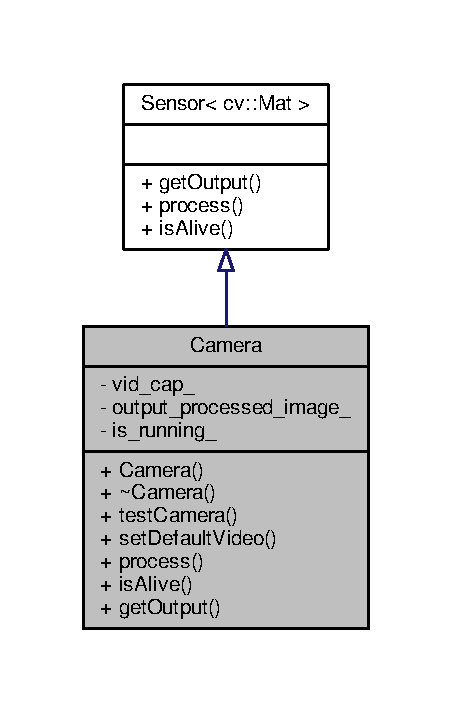
\includegraphics[width=217pt]{class_camera__inherit__graph}
\end{center}
\end{figure}
\subsection*{Public Member Functions}
\begin{DoxyCompactItemize}
\item 
\hyperlink{class_camera_a01f94c3543f56ede7af49dc778f19331}{Camera} ()
\begin{DoxyCompactList}\small\item\em Constructor of the class \hyperlink{class_camera}{Camera}. Set is\+\_\+running\+\_\+ flag to true. \end{DoxyCompactList}\item 
\hyperlink{class_camera_ad1897942d0ccf91052386388a497349f}{$\sim$\+Camera} ()
\begin{DoxyCompactList}\small\item\em Destroys the object of the class. Set is\+\_\+running\+\_\+ to false. \end{DoxyCompactList}\item 
auto \hyperlink{class_camera_ad9cc807466f09917e7f62d0d6c2e5b46}{set\+Default\+Video} () -\/$>$ bool
\begin{DoxyCompactList}\small\item\em Sets the default Video\+Capture object. Call this function if camera is not working. \end{DoxyCompactList}\item 
auto \hyperlink{class_camera_a467955a89a912bfcae67ee0905a8cd86}{test\+Camera} () -\/$>$ bool
\begin{DoxyCompactList}\small\item\em Function to test the working of camera. If the camera is not working it will set the vid\+\_\+cap\+\_\+ object to read default video. \end{DoxyCompactList}\item 
auto \hyperlink{class_camera_a3af312509cb2a7167ad0dc6280cd9207}{process} () -\/$>$ void
\begin{DoxyCompactList}\small\item\em Override the virtual method \char`\"{}process\char`\"{} of \hyperlink{class_sensor}{Sensor} class. This class processes the image so that Perception module can use it to determine the location of boundary. \end{DoxyCompactList}\item 
auto \hyperlink{class_camera_a96de7932cff3f51163250efa2762bb10}{process} (const cv\+::\+Mat \&img) -\/$>$ void
\begin{DoxyCompactList}\small\item\em Override the virtual method \char`\"{}process\char`\"{} of \hyperlink{class_sensor}{Sensor} class. This class processes the image so that Perception module can use it to determine the location of boundary. This is an overloaded function which will take an input image and process it. \end{DoxyCompactList}\item 
auto \hyperlink{class_camera_a1b3b1ece3344ea84754aff31f048d55e}{is\+Alive} () -\/$>$ bool
\begin{DoxyCompactList}\small\item\em Override the virtual method \char`\"{}is\+Alive\char`\"{} of \hyperlink{class_sensor}{Sensor} class. This method checks if the sensor is running or not. \end{DoxyCompactList}\item 
auto \hyperlink{class_camera_a456e3f62048f2266e098489a068bda0e}{get\+Output} () -\/$>$ cv\+::\+Mat
\begin{DoxyCompactList}\small\item\em Override the method \char`\"{}get\+Output\char`\"{} of \hyperlink{class_sensor}{Sensor} class. This method returns the pre-\/processed image suitable for further processing. \end{DoxyCompactList}\end{DoxyCompactItemize}
\subsection*{Private Attributes}
\begin{DoxyCompactItemize}
\item 
cv\+::\+Video\+Capture \hyperlink{class_camera_a264c7dfa5dd39176aedbb742f34ba1eb}{vid\+\_\+cap\+\_\+}
\begin{DoxyCompactList}\small\item\em Video capture object of Open\+CV. \end{DoxyCompactList}\item 
cv\+::\+Mat \hyperlink{class_camera_ae96ea8feb337852401830c24af293025}{output\+\_\+processed\+\_\+image\+\_\+}
\item 
bool \hyperlink{class_camera_a24d141601f7d0330b77b86505851bd0d}{is\+\_\+running\+\_\+}
\begin{DoxyCompactList}\small\item\em Flag to test if the camera sensor is running or not. \end{DoxyCompactList}\end{DoxyCompactItemize}


\subsection{Detailed Description}
Class for camera sensor. This class is derived from the base Class \hyperlink{class_sensor}{Sensor}. 

Definition at line 33 of file camera.\+hpp.



\subsection{Constructor \& Destructor Documentation}
\index{Camera@{Camera}!Camera@{Camera}}
\index{Camera@{Camera}!Camera@{Camera}}
\subsubsection[{\texorpdfstring{Camera()}{Camera()}}]{\setlength{\rightskip}{0pt plus 5cm}Camera\+::\+Camera (
\begin{DoxyParamCaption}
{}
\end{DoxyParamCaption}
)}\hypertarget{class_camera_a01f94c3543f56ede7af49dc778f19331}{}\label{class_camera_a01f94c3543f56ede7af49dc778f19331}


Constructor of the class \hyperlink{class_camera}{Camera}. Set is\+\_\+running\+\_\+ flag to true. 

\begin{DoxyReturn}{Returns}
void\+: Return nothing 
\end{DoxyReturn}


Definition at line 16 of file camera.\+cpp.

\index{Camera@{Camera}!````~Camera@{$\sim$\+Camera}}
\index{````~Camera@{$\sim$\+Camera}!Camera@{Camera}}
\subsubsection[{\texorpdfstring{$\sim$\+Camera()}{~Camera()}}]{\setlength{\rightskip}{0pt plus 5cm}Camera\+::$\sim$\+Camera (
\begin{DoxyParamCaption}
{}
\end{DoxyParamCaption}
)}\hypertarget{class_camera_ad1897942d0ccf91052386388a497349f}{}\label{class_camera_ad1897942d0ccf91052386388a497349f}


Destroys the object of the class. Set is\+\_\+running\+\_\+ to false. 

\begin{DoxyReturn}{Returns}
void\+: Return nothing. 
\end{DoxyReturn}


Definition at line 22 of file camera.\+cpp.



\subsection{Member Function Documentation}
\index{Camera@{Camera}!get\+Output@{get\+Output}}
\index{get\+Output@{get\+Output}!Camera@{Camera}}
\subsubsection[{\texorpdfstring{get\+Output() -\/$>$ cv\+::\+Mat}{getOutput() -> cv::Mat}}]{\setlength{\rightskip}{0pt plus 5cm}auto Camera\+::get\+Output (
\begin{DoxyParamCaption}
{}
\end{DoxyParamCaption}
) -\/$>$ cv\+::\+Mat\hspace{0.3cm}{\ttfamily [virtual]}}\hypertarget{class_camera_a456e3f62048f2266e098489a068bda0e}{}\label{class_camera_a456e3f62048f2266e098489a068bda0e}


Override the method \char`\"{}get\+Output\char`\"{} of \hyperlink{class_sensor}{Sensor} class. This method returns the pre-\/processed image suitable for further processing. 

\begin{DoxyReturn}{Returns}
cv\+::\+Mat\+: Return processed image(output\+\_\+processed\+\_\+image\+\_\+). 
\end{DoxyReturn}


Implements \hyperlink{class_sensor_abdc2eb130cb935cb090470d1fe6cc499}{Sensor$<$ cv\+::\+Mat $>$}.



Definition at line 100 of file camera.\+cpp.

\index{Camera@{Camera}!is\+Alive@{is\+Alive}}
\index{is\+Alive@{is\+Alive}!Camera@{Camera}}
\subsubsection[{\texorpdfstring{is\+Alive() -\/$>$ bool}{isAlive() -> bool}}]{\setlength{\rightskip}{0pt plus 5cm}auto Camera\+::is\+Alive (
\begin{DoxyParamCaption}
{}
\end{DoxyParamCaption}
) -\/$>$ bool\hspace{0.3cm}{\ttfamily [virtual]}}\hypertarget{class_camera_a1b3b1ece3344ea84754aff31f048d55e}{}\label{class_camera_a1b3b1ece3344ea84754aff31f048d55e}


Override the virtual method \char`\"{}is\+Alive\char`\"{} of \hyperlink{class_sensor}{Sensor} class. This method checks if the sensor is running or not. 

\begin{DoxyReturn}{Returns}
bool\+: Return \char`\"{}true\char`\"{} if the sensor is running, \char`\"{}false\char`\"{} otherwise otherwise. 
\end{DoxyReturn}


Implements \hyperlink{class_sensor_a7ae0a8c02805d3b2b8306d01da2a2db8}{Sensor$<$ cv\+::\+Mat $>$}.



Definition at line 96 of file camera.\+cpp.

\index{Camera@{Camera}!process@{process}}
\index{process@{process}!Camera@{Camera}}
\subsubsection[{\texorpdfstring{process() -\/$>$ void}{process() -> void}}]{\setlength{\rightskip}{0pt plus 5cm}auto Camera\+::process (
\begin{DoxyParamCaption}
{}
\end{DoxyParamCaption}
) -\/$>$  void}\hypertarget{class_camera_a3af312509cb2a7167ad0dc6280cd9207}{}\label{class_camera_a3af312509cb2a7167ad0dc6280cd9207}


Override the virtual method \char`\"{}process\char`\"{} of \hyperlink{class_sensor}{Sensor} class. This class processes the image so that Perception module can use it to determine the location of boundary. 

\begin{DoxyReturn}{Returns}
void\+: Return nothing. 
\end{DoxyReturn}
\index{Camera@{Camera}!process@{process}}
\index{process@{process}!Camera@{Camera}}
\subsubsection[{\texorpdfstring{process(const cv\+::\+Mat \&img) -\/$>$ void}{process(const cv::Mat &img) -> void}}]{\setlength{\rightskip}{0pt plus 5cm}auto Camera\+::process (
\begin{DoxyParamCaption}
\item[{const cv\+::\+Mat \&}]{img}
\end{DoxyParamCaption}
) -\/$>$ void}\hypertarget{class_camera_a96de7932cff3f51163250efa2762bb10}{}\label{class_camera_a96de7932cff3f51163250efa2762bb10}


Override the virtual method \char`\"{}process\char`\"{} of \hyperlink{class_sensor}{Sensor} class. This class processes the image so that Perception module can use it to determine the location of boundary. This is an overloaded function which will take an input image and process it. 


\begin{DoxyParams}[1]{Parameters}
\mbox{\tt in}  & {\em file} & Filename of the image which is to be read.\\
\hline
\end{DoxyParams}
\begin{DoxyReturn}{Returns}
void\+: Return nothing. 
\end{DoxyReturn}


Definition at line 55 of file camera.\+cpp.

\index{Camera@{Camera}!set\+Default\+Video@{set\+Default\+Video}}
\index{set\+Default\+Video@{set\+Default\+Video}!Camera@{Camera}}
\subsubsection[{\texorpdfstring{set\+Default\+Video() -\/$>$ bool}{setDefaultVideo() -> bool}}]{\setlength{\rightskip}{0pt plus 5cm}auto Camera\+::set\+Default\+Video (
\begin{DoxyParamCaption}
{}
\end{DoxyParamCaption}
) -\/$>$ bool}\hypertarget{class_camera_ad9cc807466f09917e7f62d0d6c2e5b46}{}\label{class_camera_ad9cc807466f09917e7f62d0d6c2e5b46}


Sets the default Video\+Capture object. Call this function if camera is not working. 

\begin{DoxyReturn}{Returns}
bool\+: Return true after setting the default video. 
\end{DoxyReturn}


Definition at line 47 of file camera.\+cpp.

\index{Camera@{Camera}!test\+Camera@{test\+Camera}}
\index{test\+Camera@{test\+Camera}!Camera@{Camera}}
\subsubsection[{\texorpdfstring{test\+Camera() -\/$>$ bool}{testCamera() -> bool}}]{\setlength{\rightskip}{0pt plus 5cm}auto Camera\+::test\+Camera (
\begin{DoxyParamCaption}
{}
\end{DoxyParamCaption}
) -\/$>$  bool}\hypertarget{class_camera_a467955a89a912bfcae67ee0905a8cd86}{}\label{class_camera_a467955a89a912bfcae67ee0905a8cd86}


Function to test the working of camera. If the camera is not working it will set the vid\+\_\+cap\+\_\+ object to read default video. 

\begin{DoxyReturn}{Returns}
bool\+: Return true if camera is working, false otherwise. 
\end{DoxyReturn}


\subsection{Member Data Documentation}
\index{Camera@{Camera}!is\+\_\+running\+\_\+@{is\+\_\+running\+\_\+}}
\index{is\+\_\+running\+\_\+@{is\+\_\+running\+\_\+}!Camera@{Camera}}
\subsubsection[{\texorpdfstring{is\+\_\+running\+\_\+}{is_running_}}]{\setlength{\rightskip}{0pt plus 5cm}bool Camera\+::is\+\_\+running\+\_\+\hspace{0.3cm}{\ttfamily [private]}}\hypertarget{class_camera_a24d141601f7d0330b77b86505851bd0d}{}\label{class_camera_a24d141601f7d0330b77b86505851bd0d}


Flag to test if the camera sensor is running or not. 



Definition at line 101 of file camera.\+hpp.

\index{Camera@{Camera}!output\+\_\+processed\+\_\+image\+\_\+@{output\+\_\+processed\+\_\+image\+\_\+}}
\index{output\+\_\+processed\+\_\+image\+\_\+@{output\+\_\+processed\+\_\+image\+\_\+}!Camera@{Camera}}
\subsubsection[{\texorpdfstring{output\+\_\+processed\+\_\+image\+\_\+}{output_processed_image_}}]{\setlength{\rightskip}{0pt plus 5cm}cv\+::\+Mat Camera\+::output\+\_\+processed\+\_\+image\+\_\+\hspace{0.3cm}{\ttfamily [private]}}\hypertarget{class_camera_ae96ea8feb337852401830c24af293025}{}\label{class_camera_ae96ea8feb337852401830c24af293025}
Process image which is the output of the class 

Definition at line 99 of file camera.\+hpp.

\index{Camera@{Camera}!vid\+\_\+cap\+\_\+@{vid\+\_\+cap\+\_\+}}
\index{vid\+\_\+cap\+\_\+@{vid\+\_\+cap\+\_\+}!Camera@{Camera}}
\subsubsection[{\texorpdfstring{vid\+\_\+cap\+\_\+}{vid_cap_}}]{\setlength{\rightskip}{0pt plus 5cm}cv\+::\+Video\+Capture Camera\+::vid\+\_\+cap\+\_\+\hspace{0.3cm}{\ttfamily [private]}}\hypertarget{class_camera_a264c7dfa5dd39176aedbb742f34ba1eb}{}\label{class_camera_a264c7dfa5dd39176aedbb742f34ba1eb}


Video capture object of Open\+CV. 



Definition at line 98 of file camera.\+hpp.



The documentation for this class was generated from the following files\+:\begin{DoxyCompactItemize}
\item 
/home/nrparikh/\+Desktop/acme\+\_\+robotics\+\_\+perception\+\_\+module/include/\hyperlink{camera_8hpp}{camera.\+hpp}\item 
/home/nrparikh/\+Desktop/acme\+\_\+robotics\+\_\+perception\+\_\+module/app/\hyperlink{camera_8cpp}{camera.\+cpp}\end{DoxyCompactItemize}

\hypertarget{class_control_module}{}\section{Control\+Module Class Reference}
\label{class_control_module}\index{Control\+Module@{Control\+Module}}


Class for control module. This class generates the actions based on the inputs from ultrasonic sensor and camera.  




{\ttfamily \#include $<$control\+\_\+module.\+hpp$>$}

\subsection*{Public Member Functions}
\begin{DoxyCompactItemize}
\item 
\hyperlink{class_control_module_a260b3e131b096cf456aff663aebfa6b4}{Control\+Module} ()
\begin{DoxyCompactList}\small\item\em Constructor of the class \hyperlink{class_control_module}{Control\+Module}. \end{DoxyCompactList}\item 
\hyperlink{class_control_module_ade41c6a3ce7c8e4df978c611bc0d9fa8}{$\sim$\+Control\+Module} ()
\begin{DoxyCompactList}\small\item\em Destroys the object of the class \hyperlink{class_control_module}{Control\+Module}. \end{DoxyCompactList}\item 
auto \hyperlink{class_control_module_a94f0a8b044f12df1c381655648e68aa5}{set\+Pointers} () -\/$>$ void
\begin{DoxyCompactList}\small\item\em Create the pointers to the perception and ultrasonic sensor. \end{DoxyCompactList}\item 
auto \hyperlink{class_control_module_a051b5a9bdf80ce3c21da8db10705740b}{is\+Alive} () -\/$>$ bool
\begin{DoxyCompactList}\small\item\em Determines if the module is running or not. \end{DoxyCompactList}\item 
auto \hyperlink{class_control_module_a82c3a2a8d0140432b7dd364a4388fff2}{compute\+Action\+Center} (const std\+::pair$<$ int, int $>$ \&center) -\/$>$ void
\begin{DoxyCompactList}\small\item\em Mehod to calculate the action based on the inputs. \end{DoxyCompactList}\item 
auto \hyperlink{class_control_module_a8ded8dc8ebb29333bc104a26e835ce41}{compute\+Action\+Pt} (const std\+::vector$<$ std\+::pair$<$ int, int $>$$>$ \&line\+Pts) -\/$>$ void
\begin{DoxyCompactList}\small\item\em Compute the action to be taken from the detected points on the line. \end{DoxyCompactList}\item 
auto \hyperlink{class_control_module_af623430925750c3124253b705593cdce}{get\+Control\+Action} () -\/$>$ std\+::string
\begin{DoxyCompactList}\small\item\em Gets the computed control action. \end{DoxyCompactList}\item 
auto \hyperlink{class_control_module_a10094a24e4e1e674da0bb5d0f1ef5e58}{run\+Diagnostics} () -\/$>$ bool
\begin{DoxyCompactList}\small\item\em Function to check if all the modules are running. \end{DoxyCompactList}\end{DoxyCompactItemize}
\subsection*{Private Attributes}
\begin{DoxyCompactItemize}
\item 
std\+::unique\+\_\+ptr$<$ \hyperlink{class_ultrasonic_sensor}{Ultrasonic\+Sensor} $>$ \hyperlink{class_control_module_ad446c4323ea97a807a9b355c2f121a20}{front\+\_\+sensor\+\_\+}
\begin{DoxyCompactList}\small\item\em Front distance sensor. \end{DoxyCompactList}\item 
std\+::unique\+\_\+ptr$<$ \hyperlink{class_perception_module}{Perception\+Module} $>$ \hyperlink{class_control_module_a179995b24b2400b72b2cfd079b576782}{perception\+\_\+module\+\_\+}
\begin{DoxyCompactList}\small\item\em \hyperlink{class_camera}{Camera} sensor module. \end{DoxyCompactList}\item 
std\+::string \hyperlink{class_control_module_acf268f1e0e9d27bff61e89c681a739a3}{control\+\_\+action\+\_\+}
\begin{DoxyCompactList}\small\item\em Computed control action. \end{DoxyCompactList}\item 
bool \hyperlink{class_control_module_af48419a814c008e4695bef60daf2a516}{is\+\_\+running\+\_\+}
\end{DoxyCompactItemize}


\subsection{Detailed Description}
Class for control module. This class generates the actions based on the inputs from ultrasonic sensor and camera. 

Definition at line 31 of file control\+\_\+module.\+hpp.



\subsection{Constructor \& Destructor Documentation}
\index{Control\+Module@{Control\+Module}!Control\+Module@{Control\+Module}}
\index{Control\+Module@{Control\+Module}!Control\+Module@{Control\+Module}}
\subsubsection[{\texorpdfstring{Control\+Module()}{ControlModule()}}]{\setlength{\rightskip}{0pt plus 5cm}Control\+Module\+::\+Control\+Module (
\begin{DoxyParamCaption}
{}
\end{DoxyParamCaption}
)}\hypertarget{class_control_module_a260b3e131b096cf456aff663aebfa6b4}{}\label{class_control_module_a260b3e131b096cf456aff663aebfa6b4}


Constructor of the class \hyperlink{class_control_module}{Control\+Module}. 

\begin{DoxyReturn}{Returns}
void\+: Return nothing. 
\end{DoxyReturn}


Definition at line 20 of file control\+\_\+module.\+cpp.

\index{Control\+Module@{Control\+Module}!````~Control\+Module@{$\sim$\+Control\+Module}}
\index{````~Control\+Module@{$\sim$\+Control\+Module}!Control\+Module@{Control\+Module}}
\subsubsection[{\texorpdfstring{$\sim$\+Control\+Module()}{~ControlModule()}}]{\setlength{\rightskip}{0pt plus 5cm}Control\+Module\+::$\sim$\+Control\+Module (
\begin{DoxyParamCaption}
{}
\end{DoxyParamCaption}
)}\hypertarget{class_control_module_ade41c6a3ce7c8e4df978c611bc0d9fa8}{}\label{class_control_module_ade41c6a3ce7c8e4df978c611bc0d9fa8}


Destroys the object of the class \hyperlink{class_control_module}{Control\+Module}. 



Definition at line 25 of file control\+\_\+module.\+cpp.



\subsection{Member Function Documentation}
\index{Control\+Module@{Control\+Module}!compute\+Action\+Center@{compute\+Action\+Center}}
\index{compute\+Action\+Center@{compute\+Action\+Center}!Control\+Module@{Control\+Module}}
\subsubsection[{\texorpdfstring{compute\+Action\+Center(const std\+::pair$<$ int, int $>$ \&center) -\/$>$ void}{computeActionCenter(const std::pair< int, int > &center) -> void}}]{\setlength{\rightskip}{0pt plus 5cm}auto Control\+Module\+::compute\+Action\+Center (
\begin{DoxyParamCaption}
\item[{const std\+::pair$<$ int, int $>$ \&}]{center}
\end{DoxyParamCaption}
) -\/$>$  void}\hypertarget{class_control_module_a82c3a2a8d0140432b7dd364a4388fff2}{}\label{class_control_module_a82c3a2a8d0140432b7dd364a4388fff2}


Mehod to calculate the action based on the inputs. 


\begin{DoxyParams}[1]{Parameters}
\mbox{\tt in}  & {\em center} & Center of the detected contour. \\
\hline
\mbox{\tt in}  & {\em curr\+\_\+dist} & Current distance reading.\\
\hline
\end{DoxyParams}
\begin{DoxyReturn}{Returns}
void\+: Return nothing. 
\end{DoxyReturn}
\index{Control\+Module@{Control\+Module}!compute\+Action\+Pt@{compute\+Action\+Pt}}
\index{compute\+Action\+Pt@{compute\+Action\+Pt}!Control\+Module@{Control\+Module}}
\subsubsection[{\texorpdfstring{compute\+Action\+Pt(const std\+::vector$<$ std\+::pair$<$ int, int $>$$>$ \&line\+Pts) -\/$>$ void}{computeActionPt(const std::vector< std::pair< int, int >> &linePts) -> void}}]{\setlength{\rightskip}{0pt plus 5cm}auto Control\+Module\+::compute\+Action\+Pt (
\begin{DoxyParamCaption}
\item[{const std\+::vector$<$ std\+::pair$<$ int, int $>$$>$ \&}]{line\+Pts}
\end{DoxyParamCaption}
) -\/$>$ void}\hypertarget{class_control_module_a8ded8dc8ebb29333bc104a26e835ce41}{}\label{class_control_module_a8ded8dc8ebb29333bc104a26e835ce41}


Compute the action to be taken from the detected points on the line. 


\begin{DoxyParams}[1]{Parameters}
\mbox{\tt in}  & {\em line\+Pts} & Vector of pair of points on the line\\
\hline
\end{DoxyParams}
\begin{DoxyReturn}{Returns}
void\+: Return nothing 
\end{DoxyReturn}


Definition at line 87 of file control\+\_\+module.\+cpp.

\index{Control\+Module@{Control\+Module}!get\+Control\+Action@{get\+Control\+Action}}
\index{get\+Control\+Action@{get\+Control\+Action}!Control\+Module@{Control\+Module}}
\subsubsection[{\texorpdfstring{get\+Control\+Action() -\/$>$ std\+::string}{getControlAction() -> std::string}}]{\setlength{\rightskip}{0pt plus 5cm}auto Control\+Module\+::get\+Control\+Action (
\begin{DoxyParamCaption}
{}
\end{DoxyParamCaption}
) -\/$>$ std\+::string}\hypertarget{class_control_module_af623430925750c3124253b705593cdce}{}\label{class_control_module_af623430925750c3124253b705593cdce}


Gets the computed control action. 

\begin{DoxyReturn}{Returns}
string\+: Return the computed control action. 
\end{DoxyReturn}


Definition at line 142 of file control\+\_\+module.\+cpp.

\index{Control\+Module@{Control\+Module}!is\+Alive@{is\+Alive}}
\index{is\+Alive@{is\+Alive}!Control\+Module@{Control\+Module}}
\subsubsection[{\texorpdfstring{is\+Alive() -\/$>$ bool}{isAlive() -> bool}}]{\setlength{\rightskip}{0pt plus 5cm}auto Control\+Module\+::is\+Alive (
\begin{DoxyParamCaption}
{}
\end{DoxyParamCaption}
) -\/$>$ bool}\hypertarget{class_control_module_a051b5a9bdf80ce3c21da8db10705740b}{}\label{class_control_module_a051b5a9bdf80ce3c21da8db10705740b}


Determines if the module is running or not. 

\begin{DoxyReturn}{Returns}
bool\+: Return \char`\"{}true\char`\"{} if the module is running, \char`\"{}false\char`\"{} otherwise. 
\end{DoxyReturn}


Definition at line 46 of file control\+\_\+module.\+cpp.

\index{Control\+Module@{Control\+Module}!run\+Diagnostics@{run\+Diagnostics}}
\index{run\+Diagnostics@{run\+Diagnostics}!Control\+Module@{Control\+Module}}
\subsubsection[{\texorpdfstring{run\+Diagnostics() -\/$>$ bool}{runDiagnostics() -> bool}}]{\setlength{\rightskip}{0pt plus 5cm}auto Control\+Module\+::run\+Diagnostics (
\begin{DoxyParamCaption}
{}
\end{DoxyParamCaption}
) -\/$>$ bool}\hypertarget{class_control_module_a10094a24e4e1e674da0bb5d0f1ef5e58}{}\label{class_control_module_a10094a24e4e1e674da0bb5d0f1ef5e58}


Function to check if all the modules are running. 

\begin{DoxyReturn}{Returns}
bool\+: Return true if all modules are up, false otherwise 
\end{DoxyReturn}


Definition at line 36 of file control\+\_\+module.\+cpp.

\index{Control\+Module@{Control\+Module}!set\+Pointers@{set\+Pointers}}
\index{set\+Pointers@{set\+Pointers}!Control\+Module@{Control\+Module}}
\subsubsection[{\texorpdfstring{set\+Pointers() -\/$>$ void}{setPointers() -> void}}]{\setlength{\rightskip}{0pt plus 5cm}auto Control\+Module\+::set\+Pointers (
\begin{DoxyParamCaption}
{}
\end{DoxyParamCaption}
) -\/$>$ void}\hypertarget{class_control_module_a94f0a8b044f12df1c381655648e68aa5}{}\label{class_control_module_a94f0a8b044f12df1c381655648e68aa5}


Create the pointers to the perception and ultrasonic sensor. 

\begin{DoxyReturn}{Returns}
void\+: Return nothing 
\end{DoxyReturn}


Definition at line 27 of file control\+\_\+module.\+cpp.



\subsection{Member Data Documentation}
\index{Control\+Module@{Control\+Module}!control\+\_\+action\+\_\+@{control\+\_\+action\+\_\+}}
\index{control\+\_\+action\+\_\+@{control\+\_\+action\+\_\+}!Control\+Module@{Control\+Module}}
\subsubsection[{\texorpdfstring{control\+\_\+action\+\_\+}{control_action_}}]{\setlength{\rightskip}{0pt plus 5cm}std\+::string Control\+Module\+::control\+\_\+action\+\_\+\hspace{0.3cm}{\ttfamily [private]}}\hypertarget{class_control_module_acf268f1e0e9d27bff61e89c681a739a3}{}\label{class_control_module_acf268f1e0e9d27bff61e89c681a739a3}


Computed control action. 



Definition at line 90 of file control\+\_\+module.\+hpp.

\index{Control\+Module@{Control\+Module}!front\+\_\+sensor\+\_\+@{front\+\_\+sensor\+\_\+}}
\index{front\+\_\+sensor\+\_\+@{front\+\_\+sensor\+\_\+}!Control\+Module@{Control\+Module}}
\subsubsection[{\texorpdfstring{front\+\_\+sensor\+\_\+}{front_sensor_}}]{\setlength{\rightskip}{0pt plus 5cm}std\+::unique\+\_\+ptr$<${\bf Ultrasonic\+Sensor}$>$ Control\+Module\+::front\+\_\+sensor\+\_\+\hspace{0.3cm}{\ttfamily [private]}}\hypertarget{class_control_module_ad446c4323ea97a807a9b355c2f121a20}{}\label{class_control_module_ad446c4323ea97a807a9b355c2f121a20}


Front distance sensor. 



Definition at line 87 of file control\+\_\+module.\+hpp.

\index{Control\+Module@{Control\+Module}!is\+\_\+running\+\_\+@{is\+\_\+running\+\_\+}}
\index{is\+\_\+running\+\_\+@{is\+\_\+running\+\_\+}!Control\+Module@{Control\+Module}}
\subsubsection[{\texorpdfstring{is\+\_\+running\+\_\+}{is_running_}}]{\setlength{\rightskip}{0pt plus 5cm}bool Control\+Module\+::is\+\_\+running\+\_\+\hspace{0.3cm}{\ttfamily [private]}}\hypertarget{class_control_module_af48419a814c008e4695bef60daf2a516}{}\label{class_control_module_af48419a814c008e4695bef60daf2a516}
Flag to test if the perception module is running or not. 

Definition at line 91 of file control\+\_\+module.\+hpp.

\index{Control\+Module@{Control\+Module}!perception\+\_\+module\+\_\+@{perception\+\_\+module\+\_\+}}
\index{perception\+\_\+module\+\_\+@{perception\+\_\+module\+\_\+}!Control\+Module@{Control\+Module}}
\subsubsection[{\texorpdfstring{perception\+\_\+module\+\_\+}{perception_module_}}]{\setlength{\rightskip}{0pt plus 5cm}std\+::unique\+\_\+ptr$<${\bf Perception\+Module}$>$ Control\+Module\+::perception\+\_\+module\+\_\+\hspace{0.3cm}{\ttfamily [private]}}\hypertarget{class_control_module_a179995b24b2400b72b2cfd079b576782}{}\label{class_control_module_a179995b24b2400b72b2cfd079b576782}


\hyperlink{class_camera}{Camera} sensor module. 



Definition at line 89 of file control\+\_\+module.\+hpp.



The documentation for this class was generated from the following files\+:\begin{DoxyCompactItemize}
\item 
/home/nrparikh/acme\+\_\+robotics\+\_\+perception\+\_\+module/include/\hyperlink{control__module_8hpp}{control\+\_\+module.\+hpp}\item 
/home/nrparikh/acme\+\_\+robotics\+\_\+perception\+\_\+module/app/\hyperlink{control__module_8cpp}{control\+\_\+module.\+cpp}\end{DoxyCompactItemize}

\hypertarget{class_perception_module}{}\section{Perception\+Module Class Reference}
\label{class_perception_module}\index{Perception\+Module@{Perception\+Module}}


Class for perception module. This class finds the contours and the center of the contours in the image provided as an input.  




{\ttfamily \#include $<$perception\+\_\+module.\+hpp$>$}

\subsection*{Public Member Functions}
\begin{DoxyCompactItemize}
\item 
\hyperlink{class_perception_module_a62e6934da7b7ab114c02a34e8030e0ec}{Perception\+Module} ()
\begin{DoxyCompactList}\small\item\em Constructor of the class \hyperlink{class_perception_module}{Perception\+Module}. \end{DoxyCompactList}\item 
\hyperlink{class_perception_module_a52bf1fd6688cd15a6687bc8af69bf116}{$\sim$\+Perception\+Module} ()
\begin{DoxyCompactList}\small\item\em Destroys the object of the class \hyperlink{class_perception_module}{Perception\+Module}. \end{DoxyCompactList}\item 
auto \hyperlink{class_perception_module_a60ab0780b4400096b029698b6c8f0dc7}{set\+Camera\+Obj} () -\/$>$ void
\begin{DoxyCompactList}\small\item\em Create a pointer to camera object. \end{DoxyCompactList}\item 
auto \hyperlink{class_perception_module_a934854719b0e95576883b7cb5098a7a5}{is\+Alive} () -\/$>$ bool
\begin{DoxyCompactList}\small\item\em Determines if the module is running or not. \end{DoxyCompactList}\item 
auto \hyperlink{class_perception_module_a851a7c7b5e9e11459dd171bb31128402}{detect\+Contours} (const cv\+::\+Mat \&raw\+\_\+image) -\/$>$ void
\begin{DoxyCompactList}\small\item\em Function to detect the contours in the incoming frame. \end{DoxyCompactList}\item 
auto \hyperlink{class_perception_module_ad3c7a85f300e3a545da8a619af99d4de}{detect\+Center} () -\/$>$ void
\begin{DoxyCompactList}\small\item\em Method to get the center of the detected contours. \end{DoxyCompactList}\item 
auto \hyperlink{class_perception_module_a11b2a35583209674467527ddafca2d6e}{get\+Camera\+Image} () -\/$>$ cv\+::\+Mat
\begin{DoxyCompactList}\small\item\em Gets the output image from camera. \end{DoxyCompactList}\item 
auto \hyperlink{class_perception_module_a85bf112d0310cbc6a3160e3ea24f201e}{compute\+Line\+Pts} () -\/$>$ void
\begin{DoxyCompactList}\small\item\em Finds the best fitting line using the Hough transforms and returns the points on the line. \end{DoxyCompactList}\item 
auto \hyperlink{class_perception_module_a4479a449ea05c5490a47224767a864cc}{get\+Points} () -\/$>$ std\+::vector$<$ std\+::pair$<$ int, int $>$$>$
\begin{DoxyCompactList}\small\item\em Function to return the points on the detected line. \end{DoxyCompactList}\item 
auto \hyperlink{class_perception_module_ab39e9908fda8dd1b582b33a2f1ee0638}{get\+Center} () -\/$>$ std\+::pair$<$ int, int $>$
\begin{DoxyCompactList}\small\item\em Gets the location of the center of the contour. \end{DoxyCompactList}\item 
auto \hyperlink{class_perception_module_a034e0b3191be67f571aa284e0c30f749}{camera\+Alive} () -\/$>$ bool
\begin{DoxyCompactList}\small\item\em Function to check if camera is running or not. \end{DoxyCompactList}\end{DoxyCompactItemize}
\subsection*{Private Attributes}
\begin{DoxyCompactItemize}
\item 
std\+::unique\+\_\+ptr$<$ \hyperlink{class_camera}{Camera} $>$ \hyperlink{class_perception_module_af5250548d1ab0ab5574aa17fd99104e4}{camera\+\_\+obj\+\_\+}
\begin{DoxyCompactList}\small\item\em Object of the \hyperlink{class_camera}{Camera} sensor. \end{DoxyCompactList}\item 
std\+::vector$<$ std\+::vector$<$ cv\+::\+Point $>$ $>$ \hyperlink{class_perception_module_ae611b010af7c0351eb889165198ee82a}{contours\+\_\+}
\begin{DoxyCompactList}\small\item\em Vectors of contours. \end{DoxyCompactList}\item 
std\+::vector$<$ cv\+::\+Vec4i $>$ \hyperlink{class_perception_module_a1ed5ed9b4c99dd984e76c30f25754282}{heirarchy\+\_\+}
\begin{DoxyCompactList}\small\item\em Heirarchy of contours. \end{DoxyCompactList}\item 
std\+::pair$<$ int, int $>$ \hyperlink{class_perception_module_a67ea0e9f666e33bce8d81bf22098d168}{center\+\_\+}
\item 
cv\+::\+Mat \hyperlink{class_perception_module_a4c6044231fa94975cf299e5cd60ba447}{contour\+\_\+image\+\_\+}
\begin{DoxyCompactList}\small\item\em Image containing detected contours. \end{DoxyCompactList}\item 
bool \hyperlink{class_perception_module_ab547d968284f6ab18a01b9776c54f38a}{contour\+\_\+detected\+\_\+}
\item 
int \hyperlink{class_perception_module_a7936595913566cc046bcecfe3e9803d9}{largest\+\_\+contour\+\_\+id\+\_\+}
\begin{DoxyCompactList}\small\item\em ID of the largest contour detected. \end{DoxyCompactList}\item 
float \hyperlink{class_perception_module_aa20adfc7b4a473435fc98df6353b6fd6}{largest\+\_\+contour\+\_\+area\+\_\+}
\begin{DoxyCompactList}\small\item\em Area of the largest contour detected. \end{DoxyCompactList}\item 
std\+::vector$<$ cv\+::\+Point $>$ \hyperlink{class_perception_module_a1bd3cb41f94fa253954018392a4ebdb9}{largest\+\_\+contour\+\_\+}
\begin{DoxyCompactList}\small\item\em Largest contour detected in the image. \end{DoxyCompactList}\item 
bool \hyperlink{class_perception_module_a95211a0bd4fe047b0e22e4afb7c50e26}{is\+\_\+running\+\_\+}
\item 
std\+::vector$<$ cv\+::\+Vec4i $>$ \hyperlink{class_perception_module_af7aab087aaf76ccf57ef68a8001dc530}{lines\+\_\+}
\item 
std\+::vector$<$ std\+::pair$<$ int, int $>$ $>$ \hyperlink{class_perception_module_a9cfd32e708d852e96b117e44643bbfad}{points\+\_\+}
\begin{DoxyCompactList}\small\item\em Vector of points of line. \end{DoxyCompactList}\end{DoxyCompactItemize}


\subsection{Detailed Description}
Class for perception module. This class finds the contours and the center of the contours in the image provided as an input. 

Definition at line 29 of file perception\+\_\+module.\+hpp.



\subsection{Constructor \& Destructor Documentation}
\index{Perception\+Module@{Perception\+Module}!Perception\+Module@{Perception\+Module}}
\index{Perception\+Module@{Perception\+Module}!Perception\+Module@{Perception\+Module}}
\subsubsection[{\texorpdfstring{Perception\+Module()}{PerceptionModule()}}]{\setlength{\rightskip}{0pt plus 5cm}Perception\+Module\+::\+Perception\+Module (
\begin{DoxyParamCaption}
{}
\end{DoxyParamCaption}
)}\hypertarget{class_perception_module_a62e6934da7b7ab114c02a34e8030e0ec}{}\label{class_perception_module_a62e6934da7b7ab114c02a34e8030e0ec}


Constructor of the class \hyperlink{class_perception_module}{Perception\+Module}. 

\begin{DoxyReturn}{Returns}
void\+: Return nothing. 
\end{DoxyReturn}


Definition at line 21 of file perception\+\_\+module.\+cpp.

\index{Perception\+Module@{Perception\+Module}!````~Perception\+Module@{$\sim$\+Perception\+Module}}
\index{````~Perception\+Module@{$\sim$\+Perception\+Module}!Perception\+Module@{Perception\+Module}}
\subsubsection[{\texorpdfstring{$\sim$\+Perception\+Module()}{~PerceptionModule()}}]{\setlength{\rightskip}{0pt plus 5cm}Perception\+Module\+::$\sim$\+Perception\+Module (
\begin{DoxyParamCaption}
{}
\end{DoxyParamCaption}
)}\hypertarget{class_perception_module_a52bf1fd6688cd15a6687bc8af69bf116}{}\label{class_perception_module_a52bf1fd6688cd15a6687bc8af69bf116}


Destroys the object of the class \hyperlink{class_perception_module}{Perception\+Module}. 

\begin{DoxyReturn}{Returns}
void\+: Return nothing. 
\end{DoxyReturn}


Definition at line 29 of file perception\+\_\+module.\+cpp.



\subsection{Member Function Documentation}
\index{Perception\+Module@{Perception\+Module}!camera\+Alive@{camera\+Alive}}
\index{camera\+Alive@{camera\+Alive}!Perception\+Module@{Perception\+Module}}
\subsubsection[{\texorpdfstring{camera\+Alive() -\/$>$ bool}{cameraAlive() -> bool}}]{\setlength{\rightskip}{0pt plus 5cm}auto Perception\+Module\+::camera\+Alive (
\begin{DoxyParamCaption}
{}
\end{DoxyParamCaption}
) -\/$>$ bool}\hypertarget{class_perception_module_a034e0b3191be67f571aa284e0c30f749}{}\label{class_perception_module_a034e0b3191be67f571aa284e0c30f749}


Function to check if camera is running or not. 

\begin{DoxyReturn}{Returns}
bool\+: Return the value returned by \hyperlink{class_camera_a1b3b1ece3344ea84754aff31f048d55e}{Camera\+::is\+Alive} 
\end{DoxyReturn}


Definition at line 153 of file perception\+\_\+module.\+cpp.

\index{Perception\+Module@{Perception\+Module}!compute\+Line\+Pts@{compute\+Line\+Pts}}
\index{compute\+Line\+Pts@{compute\+Line\+Pts}!Perception\+Module@{Perception\+Module}}
\subsubsection[{\texorpdfstring{compute\+Line\+Pts() -\/$>$ void}{computeLinePts() -> void}}]{\setlength{\rightskip}{0pt plus 5cm}auto Perception\+Module\+::compute\+Line\+Pts (
\begin{DoxyParamCaption}
{}
\end{DoxyParamCaption}
) -\/$>$ void}\hypertarget{class_perception_module_a85bf112d0310cbc6a3160e3ea24f201e}{}\label{class_perception_module_a85bf112d0310cbc6a3160e3ea24f201e}


Finds the best fitting line using the Hough transforms and returns the points on the line. 

\begin{DoxyReturn}{Returns}
void\+: Return nothing 
\end{DoxyReturn}


Definition at line 106 of file perception\+\_\+module.\+cpp.

\index{Perception\+Module@{Perception\+Module}!detect\+Center@{detect\+Center}}
\index{detect\+Center@{detect\+Center}!Perception\+Module@{Perception\+Module}}
\subsubsection[{\texorpdfstring{detect\+Center() -\/$>$ void}{detectCenter() -> void}}]{\setlength{\rightskip}{0pt plus 5cm}auto Perception\+Module\+::detect\+Center (
\begin{DoxyParamCaption}
{}
\end{DoxyParamCaption}
) -\/$>$  void}\hypertarget{class_perception_module_ad3c7a85f300e3a545da8a619af99d4de}{}\label{class_perception_module_ad3c7a85f300e3a545da8a619af99d4de}


Method to get the center of the detected contours. 


\begin{DoxyParams}[1]{Parameters}
\mbox{\tt in}  & {\em raw\+\_\+image} & The image which is to be processed.\\
\hline
\end{DoxyParams}
\begin{DoxyReturn}{Returns}
void\+: Return nothing. 
\end{DoxyReturn}
\index{Perception\+Module@{Perception\+Module}!detect\+Contours@{detect\+Contours}}
\index{detect\+Contours@{detect\+Contours}!Perception\+Module@{Perception\+Module}}
\subsubsection[{\texorpdfstring{detect\+Contours(const cv\+::\+Mat \&raw\+\_\+image) -\/$>$ void}{detectContours(const cv::Mat &raw_image) -> void}}]{\setlength{\rightskip}{0pt plus 5cm}auto Perception\+Module\+::detect\+Contours (
\begin{DoxyParamCaption}
\item[{const cv\+::\+Mat \&}]{raw\+\_\+image}
\end{DoxyParamCaption}
) -\/$>$  void}\hypertarget{class_perception_module_a851a7c7b5e9e11459dd171bb31128402}{}\label{class_perception_module_a851a7c7b5e9e11459dd171bb31128402}


Function to detect the contours in the incoming frame. 


\begin{DoxyParams}[1]{Parameters}
\mbox{\tt in}  & {\em raw\+\_\+image} & The image in which contours are to be found.\\
\hline
\end{DoxyParams}
\begin{DoxyReturn}{Returns}
void\+: Return nothing. 
\end{DoxyReturn}
\index{Perception\+Module@{Perception\+Module}!get\+Camera\+Image@{get\+Camera\+Image}}
\index{get\+Camera\+Image@{get\+Camera\+Image}!Perception\+Module@{Perception\+Module}}
\subsubsection[{\texorpdfstring{get\+Camera\+Image() -\/$>$ cv\+::\+Mat}{getCameraImage() -> cv::Mat}}]{\setlength{\rightskip}{0pt plus 5cm}auto Perception\+Module\+::get\+Camera\+Image (
\begin{DoxyParamCaption}
{}
\end{DoxyParamCaption}
) -\/$>$ cv\+::\+Mat}\hypertarget{class_perception_module_a11b2a35583209674467527ddafca2d6e}{}\label{class_perception_module_a11b2a35583209674467527ddafca2d6e}


Gets the output image from camera. 

\begin{DoxyReturn}{Returns}
cv\+::\+Mat\+: Return the output image from camera. 
\end{DoxyReturn}


Definition at line 140 of file perception\+\_\+module.\+cpp.

\index{Perception\+Module@{Perception\+Module}!get\+Center@{get\+Center}}
\index{get\+Center@{get\+Center}!Perception\+Module@{Perception\+Module}}
\subsubsection[{\texorpdfstring{get\+Center() -\/$>$ std\+::pair$<$ int, int $>$}{getCenter() -> std::pair< int, int >}}]{\setlength{\rightskip}{0pt plus 5cm}auto Perception\+Module\+::get\+Center (
\begin{DoxyParamCaption}
{}
\end{DoxyParamCaption}
) -\/$>$  std\+::pair$<$ int, int $>$}\hypertarget{class_perception_module_ab39e9908fda8dd1b582b33a2f1ee0638}{}\label{class_perception_module_ab39e9908fda8dd1b582b33a2f1ee0638}


Gets the location of the center of the contour. 

\begin{DoxyReturn}{Returns}
std\+::pair$<$int$>$\+: Return the center of the contour. 
\end{DoxyReturn}
\index{Perception\+Module@{Perception\+Module}!get\+Points@{get\+Points}}
\index{get\+Points@{get\+Points}!Perception\+Module@{Perception\+Module}}
\subsubsection[{\texorpdfstring{get\+Points() -\/$>$ std\+::vector$<$ std\+::pair$<$ int, int $>$$>$}{getPoints() -> std::vector< std::pair< int, int >>}}]{\setlength{\rightskip}{0pt plus 5cm}auto Perception\+Module\+::get\+Points (
\begin{DoxyParamCaption}
{}
\end{DoxyParamCaption}
) -\/$>$ std\+::vector$<$std\+::pair$<$int, int$>$$>$}\hypertarget{class_perception_module_a4479a449ea05c5490a47224767a864cc}{}\label{class_perception_module_a4479a449ea05c5490a47224767a864cc}


Function to return the points on the detected line. 

\begin{DoxyReturn}{Returns}
std\+::vector$<$std\+::pair$<$int, int$>$$>$\+: Return vector of pair of the points on the detected line. 
\end{DoxyReturn}


Definition at line 147 of file perception\+\_\+module.\+cpp.

\index{Perception\+Module@{Perception\+Module}!is\+Alive@{is\+Alive}}
\index{is\+Alive@{is\+Alive}!Perception\+Module@{Perception\+Module}}
\subsubsection[{\texorpdfstring{is\+Alive() -\/$>$ bool}{isAlive() -> bool}}]{\setlength{\rightskip}{0pt plus 5cm}auto Perception\+Module\+::is\+Alive (
\begin{DoxyParamCaption}
{}
\end{DoxyParamCaption}
) -\/$>$ bool}\hypertarget{class_perception_module_a934854719b0e95576883b7cb5098a7a5}{}\label{class_perception_module_a934854719b0e95576883b7cb5098a7a5}


Determines if the module is running or not. 

\begin{DoxyReturn}{Returns}
bool\+: Return \char`\"{}true\char`\"{} if the module is running, \char`\"{}false\char`\"{} otherwise. 
\end{DoxyReturn}


Definition at line 36 of file perception\+\_\+module.\+cpp.

\index{Perception\+Module@{Perception\+Module}!set\+Camera\+Obj@{set\+Camera\+Obj}}
\index{set\+Camera\+Obj@{set\+Camera\+Obj}!Perception\+Module@{Perception\+Module}}
\subsubsection[{\texorpdfstring{set\+Camera\+Obj() -\/$>$ void}{setCameraObj() -> void}}]{\setlength{\rightskip}{0pt plus 5cm}auto Perception\+Module\+::set\+Camera\+Obj (
\begin{DoxyParamCaption}
{}
\end{DoxyParamCaption}
) -\/$>$ void}\hypertarget{class_perception_module_a60ab0780b4400096b029698b6c8f0dc7}{}\label{class_perception_module_a60ab0780b4400096b029698b6c8f0dc7}


Create a pointer to camera object. 

\begin{DoxyReturn}{Returns}
void\+: Return nothing 
\end{DoxyReturn}


Definition at line 31 of file perception\+\_\+module.\+cpp.



\subsection{Member Data Documentation}
\index{Perception\+Module@{Perception\+Module}!camera\+\_\+obj\+\_\+@{camera\+\_\+obj\+\_\+}}
\index{camera\+\_\+obj\+\_\+@{camera\+\_\+obj\+\_\+}!Perception\+Module@{Perception\+Module}}
\subsubsection[{\texorpdfstring{camera\+\_\+obj\+\_\+}{camera_obj_}}]{\setlength{\rightskip}{0pt plus 5cm}std\+::unique\+\_\+ptr$<${\bf Camera}$>$ Perception\+Module\+::camera\+\_\+obj\+\_\+\hspace{0.3cm}{\ttfamily [private]}}\hypertarget{class_perception_module_af5250548d1ab0ab5574aa17fd99104e4}{}\label{class_perception_module_af5250548d1ab0ab5574aa17fd99104e4}


Object of the \hyperlink{class_camera}{Camera} sensor. 



Definition at line 106 of file perception\+\_\+module.\+hpp.

\index{Perception\+Module@{Perception\+Module}!center\+\_\+@{center\+\_\+}}
\index{center\+\_\+@{center\+\_\+}!Perception\+Module@{Perception\+Module}}
\subsubsection[{\texorpdfstring{center\+\_\+}{center_}}]{\setlength{\rightskip}{0pt plus 5cm}std\+::pair$<$int, int$>$ Perception\+Module\+::center\+\_\+\hspace{0.3cm}{\ttfamily [private]}}\hypertarget{class_perception_module_a67ea0e9f666e33bce8d81bf22098d168}{}\label{class_perception_module_a67ea0e9f666e33bce8d81bf22098d168}


Definition at line 109 of file perception\+\_\+module.\+hpp.

\index{Perception\+Module@{Perception\+Module}!contour\+\_\+detected\+\_\+@{contour\+\_\+detected\+\_\+}}
\index{contour\+\_\+detected\+\_\+@{contour\+\_\+detected\+\_\+}!Perception\+Module@{Perception\+Module}}
\subsubsection[{\texorpdfstring{contour\+\_\+detected\+\_\+}{contour_detected_}}]{\setlength{\rightskip}{0pt plus 5cm}bool Perception\+Module\+::contour\+\_\+detected\+\_\+\hspace{0.3cm}{\ttfamily [private]}}\hypertarget{class_perception_module_ab547d968284f6ab18a01b9776c54f38a}{}\label{class_perception_module_ab547d968284f6ab18a01b9776c54f38a}
Flag to indicated whether the contour is detected or not. 

Definition at line 111 of file perception\+\_\+module.\+hpp.

\index{Perception\+Module@{Perception\+Module}!contour\+\_\+image\+\_\+@{contour\+\_\+image\+\_\+}}
\index{contour\+\_\+image\+\_\+@{contour\+\_\+image\+\_\+}!Perception\+Module@{Perception\+Module}}
\subsubsection[{\texorpdfstring{contour\+\_\+image\+\_\+}{contour_image_}}]{\setlength{\rightskip}{0pt plus 5cm}cv\+::\+Mat Perception\+Module\+::contour\+\_\+image\+\_\+\hspace{0.3cm}{\ttfamily [private]}}\hypertarget{class_perception_module_a4c6044231fa94975cf299e5cd60ba447}{}\label{class_perception_module_a4c6044231fa94975cf299e5cd60ba447}


Image containing detected contours. 



Definition at line 110 of file perception\+\_\+module.\+hpp.

\index{Perception\+Module@{Perception\+Module}!contours\+\_\+@{contours\+\_\+}}
\index{contours\+\_\+@{contours\+\_\+}!Perception\+Module@{Perception\+Module}}
\subsubsection[{\texorpdfstring{contours\+\_\+}{contours_}}]{\setlength{\rightskip}{0pt plus 5cm}std\+::vector$<$std\+::vector$<$cv\+::\+Point$>$ $>$ Perception\+Module\+::contours\+\_\+\hspace{0.3cm}{\ttfamily [private]}}\hypertarget{class_perception_module_ae611b010af7c0351eb889165198ee82a}{}\label{class_perception_module_ae611b010af7c0351eb889165198ee82a}


Vectors of contours. 



Definition at line 107 of file perception\+\_\+module.\+hpp.

\index{Perception\+Module@{Perception\+Module}!heirarchy\+\_\+@{heirarchy\+\_\+}}
\index{heirarchy\+\_\+@{heirarchy\+\_\+}!Perception\+Module@{Perception\+Module}}
\subsubsection[{\texorpdfstring{heirarchy\+\_\+}{heirarchy_}}]{\setlength{\rightskip}{0pt plus 5cm}std\+::vector$<$cv\+::\+Vec4i$>$ Perception\+Module\+::heirarchy\+\_\+\hspace{0.3cm}{\ttfamily [private]}}\hypertarget{class_perception_module_a1ed5ed9b4c99dd984e76c30f25754282}{}\label{class_perception_module_a1ed5ed9b4c99dd984e76c30f25754282}


Heirarchy of contours. 



Definition at line 108 of file perception\+\_\+module.\+hpp.

\index{Perception\+Module@{Perception\+Module}!is\+\_\+running\+\_\+@{is\+\_\+running\+\_\+}}
\index{is\+\_\+running\+\_\+@{is\+\_\+running\+\_\+}!Perception\+Module@{Perception\+Module}}
\subsubsection[{\texorpdfstring{is\+\_\+running\+\_\+}{is_running_}}]{\setlength{\rightskip}{0pt plus 5cm}bool Perception\+Module\+::is\+\_\+running\+\_\+\hspace{0.3cm}{\ttfamily [private]}}\hypertarget{class_perception_module_a95211a0bd4fe047b0e22e4afb7c50e26}{}\label{class_perception_module_a95211a0bd4fe047b0e22e4afb7c50e26}
Flag to test if the perception module is running or not. 

Definition at line 117 of file perception\+\_\+module.\+hpp.

\index{Perception\+Module@{Perception\+Module}!largest\+\_\+contour\+\_\+@{largest\+\_\+contour\+\_\+}}
\index{largest\+\_\+contour\+\_\+@{largest\+\_\+contour\+\_\+}!Perception\+Module@{Perception\+Module}}
\subsubsection[{\texorpdfstring{largest\+\_\+contour\+\_\+}{largest_contour_}}]{\setlength{\rightskip}{0pt plus 5cm}std\+::vector$<$cv\+::\+Point$>$ Perception\+Module\+::largest\+\_\+contour\+\_\+\hspace{0.3cm}{\ttfamily [private]}}\hypertarget{class_perception_module_a1bd3cb41f94fa253954018392a4ebdb9}{}\label{class_perception_module_a1bd3cb41f94fa253954018392a4ebdb9}


Largest contour detected in the image. 



Definition at line 116 of file perception\+\_\+module.\+hpp.

\index{Perception\+Module@{Perception\+Module}!largest\+\_\+contour\+\_\+area\+\_\+@{largest\+\_\+contour\+\_\+area\+\_\+}}
\index{largest\+\_\+contour\+\_\+area\+\_\+@{largest\+\_\+contour\+\_\+area\+\_\+}!Perception\+Module@{Perception\+Module}}
\subsubsection[{\texorpdfstring{largest\+\_\+contour\+\_\+area\+\_\+}{largest_contour_area_}}]{\setlength{\rightskip}{0pt plus 5cm}float Perception\+Module\+::largest\+\_\+contour\+\_\+area\+\_\+\hspace{0.3cm}{\ttfamily [private]}}\hypertarget{class_perception_module_aa20adfc7b4a473435fc98df6353b6fd6}{}\label{class_perception_module_aa20adfc7b4a473435fc98df6353b6fd6}


Area of the largest contour detected. 



Definition at line 114 of file perception\+\_\+module.\+hpp.

\index{Perception\+Module@{Perception\+Module}!largest\+\_\+contour\+\_\+id\+\_\+@{largest\+\_\+contour\+\_\+id\+\_\+}}
\index{largest\+\_\+contour\+\_\+id\+\_\+@{largest\+\_\+contour\+\_\+id\+\_\+}!Perception\+Module@{Perception\+Module}}
\subsubsection[{\texorpdfstring{largest\+\_\+contour\+\_\+id\+\_\+}{largest_contour_id_}}]{\setlength{\rightskip}{0pt plus 5cm}int Perception\+Module\+::largest\+\_\+contour\+\_\+id\+\_\+\hspace{0.3cm}{\ttfamily [private]}}\hypertarget{class_perception_module_a7936595913566cc046bcecfe3e9803d9}{}\label{class_perception_module_a7936595913566cc046bcecfe3e9803d9}


ID of the largest contour detected. 



Definition at line 113 of file perception\+\_\+module.\+hpp.

\index{Perception\+Module@{Perception\+Module}!lines\+\_\+@{lines\+\_\+}}
\index{lines\+\_\+@{lines\+\_\+}!Perception\+Module@{Perception\+Module}}
\subsubsection[{\texorpdfstring{lines\+\_\+}{lines_}}]{\setlength{\rightskip}{0pt plus 5cm}std\+::vector$<$cv\+::\+Vec4i$>$ Perception\+Module\+::lines\+\_\+\hspace{0.3cm}{\ttfamily [private]}}\hypertarget{class_perception_module_af7aab087aaf76ccf57ef68a8001dc530}{}\label{class_perception_module_af7aab087aaf76ccf57ef68a8001dc530}


Definition at line 119 of file perception\+\_\+module.\+hpp.

\index{Perception\+Module@{Perception\+Module}!points\+\_\+@{points\+\_\+}}
\index{points\+\_\+@{points\+\_\+}!Perception\+Module@{Perception\+Module}}
\subsubsection[{\texorpdfstring{points\+\_\+}{points_}}]{\setlength{\rightskip}{0pt plus 5cm}std\+::vector$<$std\+::pair$<$int, int$>$ $>$ Perception\+Module\+::points\+\_\+\hspace{0.3cm}{\ttfamily [private]}}\hypertarget{class_perception_module_a9cfd32e708d852e96b117e44643bbfad}{}\label{class_perception_module_a9cfd32e708d852e96b117e44643bbfad}


Vector of points of line. 



Definition at line 120 of file perception\+\_\+module.\+hpp.



The documentation for this class was generated from the following files\+:\begin{DoxyCompactItemize}
\item 
/home/nrparikh/acme\+\_\+robotics\+\_\+perception\+\_\+module/include/\hyperlink{perception__module_8hpp}{perception\+\_\+module.\+hpp}\item 
/home/nrparikh/acme\+\_\+robotics\+\_\+perception\+\_\+module/app/\hyperlink{perception__module_8cpp}{perception\+\_\+module.\+cpp}\end{DoxyCompactItemize}

\hypertarget{class_sensor}{}\section{Sensor$<$ T $>$ Class Template Reference}
\label{class_sensor}\index{Sensor$<$ T $>$@{Sensor$<$ T $>$}}


Class for generic sensor. Particular sensor in the system will inherit this base class.  




{\ttfamily \#include $<$sensor.\+hpp$>$}

\subsection*{Public Member Functions}
\begin{DoxyCompactItemize}
\item 
virtual auto \hyperlink{class_sensor_abdc2eb130cb935cb090470d1fe6cc499}{get\+Output} () -\/$>$ T=0
\begin{DoxyCompactList}\small\item\em Function to get the output variables of the class. \end{DoxyCompactList}\item 
virtual auto \hyperlink{class_sensor_a6482196cbd29fb6bdc0b03d8af26d501}{process} () -\/$>$ void=0
\begin{DoxyCompactList}\small\item\em Function to do the process of respective class. \end{DoxyCompactList}\item 
virtual auto \hyperlink{class_sensor_a7ae0a8c02805d3b2b8306d01da2a2db8}{is\+Alive} () -\/$>$ bool=0
\begin{DoxyCompactList}\small\item\em Function to check whether the sensor is running. \end{DoxyCompactList}\end{DoxyCompactItemize}


\subsection{Detailed Description}
\subsubsection*{template$<$class T$>$\\*
class Sensor$<$ T $>$}

Class for generic sensor. Particular sensor in the system will inherit this base class. 

Definition at line 22 of file sensor.\+hpp.



\subsection{Member Function Documentation}
\index{Sensor@{Sensor}!get\+Output@{get\+Output}}
\index{get\+Output@{get\+Output}!Sensor@{Sensor}}
\subsubsection[{\texorpdfstring{get\+Output() -\/$>$ T=0}{getOutput() -> T=0}}]{\setlength{\rightskip}{0pt plus 5cm}template$<$class T$>$ virtual auto {\bf Sensor}$<$ T $>$\+::get\+Output (
\begin{DoxyParamCaption}
{}
\end{DoxyParamCaption}
) -\/$>$  T\hspace{0.3cm}{\ttfamily [pure virtual]}}\hypertarget{class_sensor_abdc2eb130cb935cb090470d1fe6cc499}{}\label{class_sensor_abdc2eb130cb935cb090470d1fe6cc499}


Function to get the output variables of the class. 

\begin{DoxyReturn}{Returns}
void\+: Return nothing 
\end{DoxyReturn}


Implemented in \hyperlink{class_ultrasonic_sensor_a0776a669d6c30958fe316cb2daa3e6e7}{Ultrasonic\+Sensor}, and \hyperlink{class_camera_a456e3f62048f2266e098489a068bda0e}{Camera}.

\index{Sensor@{Sensor}!is\+Alive@{is\+Alive}}
\index{is\+Alive@{is\+Alive}!Sensor@{Sensor}}
\subsubsection[{\texorpdfstring{is\+Alive() -\/$>$ bool=0}{isAlive() -> bool=0}}]{\setlength{\rightskip}{0pt plus 5cm}template$<$class T$>$ virtual auto {\bf Sensor}$<$ T $>$\+::is\+Alive (
\begin{DoxyParamCaption}
{}
\end{DoxyParamCaption}
) -\/$>$  bool\hspace{0.3cm}{\ttfamily [pure virtual]}}\hypertarget{class_sensor_a7ae0a8c02805d3b2b8306d01da2a2db8}{}\label{class_sensor_a7ae0a8c02805d3b2b8306d01da2a2db8}


Function to check whether the sensor is running. 

\begin{DoxyReturn}{Returns}
bool\+: Return \char`\"{}true\char`\"{} if running, \char`\"{}false\char`\"{} otherwise 
\end{DoxyReturn}


Implemented in \hyperlink{class_camera_a1b3b1ece3344ea84754aff31f048d55e}{Camera}, and \hyperlink{class_ultrasonic_sensor_af10dfe88aa79e9c108055d5b4b5144e9}{Ultrasonic\+Sensor}.

\index{Sensor@{Sensor}!process@{process}}
\index{process@{process}!Sensor@{Sensor}}
\subsubsection[{\texorpdfstring{process() -\/$>$ void=0}{process() -> void=0}}]{\setlength{\rightskip}{0pt plus 5cm}template$<$class T$>$ virtual auto {\bf Sensor}$<$ T $>$\+::process (
\begin{DoxyParamCaption}
{}
\end{DoxyParamCaption}
) -\/$>$  void\hspace{0.3cm}{\ttfamily [pure virtual]}}\hypertarget{class_sensor_a6482196cbd29fb6bdc0b03d8af26d501}{}\label{class_sensor_a6482196cbd29fb6bdc0b03d8af26d501}


Function to do the process of respective class. 

\begin{DoxyReturn}{Returns}
void\+: Return nothing 
\end{DoxyReturn}


Implemented in \hyperlink{class_camera_a3af312509cb2a7167ad0dc6280cd9207}{Camera}, and \hyperlink{class_ultrasonic_sensor_af20b33a57f5b4522566d6856f6ca4428}{Ultrasonic\+Sensor}.



The documentation for this class was generated from the following file\+:\begin{DoxyCompactItemize}
\item 
/home/nrparikh/acme\+\_\+robotics\+\_\+perception\+\_\+module/include/\hyperlink{sensor_8hpp}{sensor.\+hpp}\end{DoxyCompactItemize}

\hypertarget{class_test_camera}{}\section{Test\+Camera Class Reference}
\label{class_test_camera}\index{Test\+Camera@{Test\+Camera}}


Class for the testing of \hyperlink{class_camera}{Camera} class. Creates a protected camera object which can be used for testing.  




Inheritance diagram for Test\+Camera\+:
\nopagebreak
\begin{figure}[H]
\begin{center}
\leavevmode
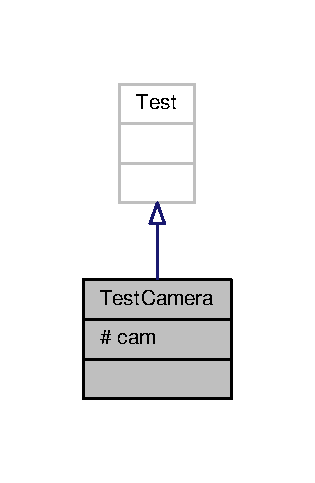
\includegraphics[width=151pt]{class_test_camera__inherit__graph}
\end{center}
\end{figure}
\subsection*{Protected Attributes}
\begin{DoxyCompactItemize}
\item 
\hyperlink{class_camera}{Camera} \hyperlink{class_test_camera_ac1abc17c2f7f776456583bc3a60db3a9}{cam}
\end{DoxyCompactItemize}


\subsection{Detailed Description}
Class for the testing of \hyperlink{class_camera}{Camera} class. Creates a protected camera object which can be used for testing. 

Definition at line 20 of file test\+\_\+camera.\+cpp.



\subsection{Member Data Documentation}
\index{Test\+Camera@{Test\+Camera}!cam@{cam}}
\index{cam@{cam}!Test\+Camera@{Test\+Camera}}
\subsubsection[{\texorpdfstring{cam}{cam}}]{\setlength{\rightskip}{0pt plus 5cm}{\bf Camera} Test\+Camera\+::cam\hspace{0.3cm}{\ttfamily [protected]}}\hypertarget{class_test_camera_ac1abc17c2f7f776456583bc3a60db3a9}{}\label{class_test_camera_ac1abc17c2f7f776456583bc3a60db3a9}


Definition at line 22 of file test\+\_\+camera.\+cpp.



The documentation for this class was generated from the following file\+:\begin{DoxyCompactItemize}
\item 
/home/nrparikh/acme\+\_\+robotics\+\_\+perception\+\_\+module/test/\hyperlink{test__camera_8cpp}{test\+\_\+camera.\+cpp}\end{DoxyCompactItemize}

\hypertarget{class_test_control_module}{}\section{Test\+Control\+Module Class Reference}
\label{class_test_control_module}\index{Test\+Control\+Module@{Test\+Control\+Module}}


Class for testing the \hyperlink{class_control_module}{Control\+Module} of the code. Create instances of perception and control modules which can be used later for testing.  




Inheritance diagram for Test\+Control\+Module\+:\nopagebreak
\begin{figure}[H]
\begin{center}
\leavevmode
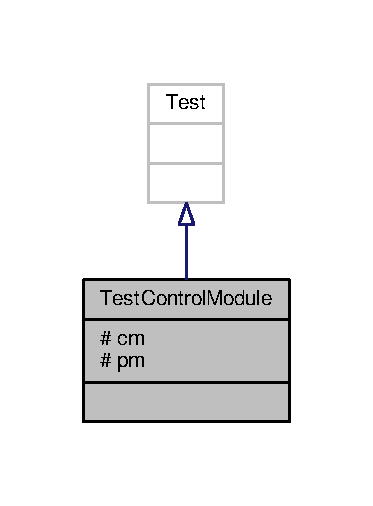
\includegraphics[width=179pt]{class_test_control_module__inherit__graph}
\end{center}
\end{figure}
\subsection*{Protected Attributes}
\begin{DoxyCompactItemize}
\item 
\hyperlink{class_control_module}{Control\+Module} \hyperlink{class_test_control_module_a8b31203bb99dac1486c80c5c270673a3}{cm}
\item 
\hyperlink{class_perception_module}{Perception\+Module} \hyperlink{class_test_control_module_ad498100deff15c962c1d6e933901f7cf}{pm}
\end{DoxyCompactItemize}


\subsection{Detailed Description}
Class for testing the \hyperlink{class_control_module}{Control\+Module} of the code. Create instances of perception and control modules which can be used later for testing. 

Definition at line 18 of file test\+\_\+control\+\_\+module.\+cpp.



\subsection{Member Data Documentation}
\index{Test\+Control\+Module@{Test\+Control\+Module}!cm@{cm}}
\index{cm@{cm}!Test\+Control\+Module@{Test\+Control\+Module}}
\subsubsection[{\texorpdfstring{cm}{cm}}]{\setlength{\rightskip}{0pt plus 5cm}{\bf Control\+Module} Test\+Control\+Module\+::cm\hspace{0.3cm}{\ttfamily [protected]}}\hypertarget{class_test_control_module_a8b31203bb99dac1486c80c5c270673a3}{}\label{class_test_control_module_a8b31203bb99dac1486c80c5c270673a3}


Definition at line 20 of file test\+\_\+control\+\_\+module.\+cpp.

\index{Test\+Control\+Module@{Test\+Control\+Module}!pm@{pm}}
\index{pm@{pm}!Test\+Control\+Module@{Test\+Control\+Module}}
\subsubsection[{\texorpdfstring{pm}{pm}}]{\setlength{\rightskip}{0pt plus 5cm}{\bf Perception\+Module} Test\+Control\+Module\+::pm\hspace{0.3cm}{\ttfamily [protected]}}\hypertarget{class_test_control_module_ad498100deff15c962c1d6e933901f7cf}{}\label{class_test_control_module_ad498100deff15c962c1d6e933901f7cf}


Definition at line 21 of file test\+\_\+control\+\_\+module.\+cpp.



The documentation for this class was generated from the following file\+:\begin{DoxyCompactItemize}
\item 
/home/nrparikh/\+Desktop/acme\+\_\+robotics\+\_\+perception\+\_\+module/test/\hyperlink{test__control__module_8cpp}{test\+\_\+control\+\_\+module.\+cpp}\end{DoxyCompactItemize}

\hypertarget{class_test_perception_module}{}\section{Test\+Perception\+Module Class Reference}
\label{class_test_perception_module}\index{Test\+Perception\+Module@{Test\+Perception\+Module}}


Class to test the working of \hyperlink{class_perception_module}{Perception\+Module}. Create an instance of perception module which can be used for testing.  




Inheritance diagram for Test\+Perception\+Module\+:\nopagebreak
\begin{figure}[H]
\begin{center}
\leavevmode
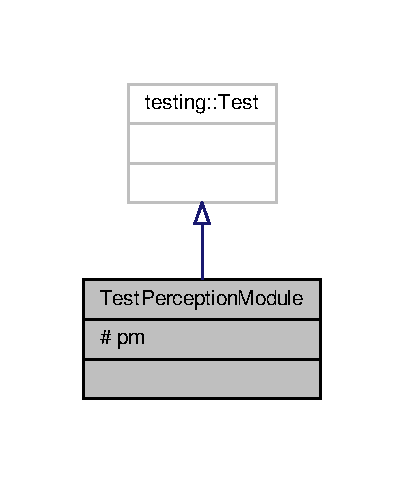
\includegraphics[width=194pt]{class_test_perception_module__inherit__graph}
\end{center}
\end{figure}
\subsection*{Protected Attributes}
\begin{DoxyCompactItemize}
\item 
\hyperlink{class_perception_module}{Perception\+Module} \hyperlink{class_test_perception_module_a71860459e03b86cd747f283436bcd757}{pm}
\end{DoxyCompactItemize}


\subsection{Detailed Description}
Class to test the working of \hyperlink{class_perception_module}{Perception\+Module}. Create an instance of perception module which can be used for testing. 

Definition at line 17 of file test\+\_\+perception\+\_\+module.\+cpp.



\subsection{Member Data Documentation}
\index{Test\+Perception\+Module@{Test\+Perception\+Module}!pm@{pm}}
\index{pm@{pm}!Test\+Perception\+Module@{Test\+Perception\+Module}}
\subsubsection[{\texorpdfstring{pm}{pm}}]{\setlength{\rightskip}{0pt plus 5cm}{\bf Perception\+Module} Test\+Perception\+Module\+::pm\hspace{0.3cm}{\ttfamily [protected]}}\hypertarget{class_test_perception_module_a71860459e03b86cd747f283436bcd757}{}\label{class_test_perception_module_a71860459e03b86cd747f283436bcd757}


Definition at line 19 of file test\+\_\+perception\+\_\+module.\+cpp.



The documentation for this class was generated from the following file\+:\begin{DoxyCompactItemize}
\item 
/home/nrparikh/\+Desktop/acme\+\_\+robotics\+\_\+perception\+\_\+module/test/\hyperlink{test__perception__module_8cpp}{test\+\_\+perception\+\_\+module.\+cpp}\end{DoxyCompactItemize}

\hypertarget{class_test_ultrasonic_sensor}{}\section{Test\+Ultrasonic\+Sensor Class Reference}
\label{class_test_ultrasonic_sensor}\index{Test\+Ultrasonic\+Sensor@{Test\+Ultrasonic\+Sensor}}


Class to test the working of Ultrasonic sensor. Create an instance of ultrasonic sensor which can be used for testing.  




Inheritance diagram for Test\+Ultrasonic\+Sensor\+:\nopagebreak
\begin{figure}[H]
\begin{center}
\leavevmode
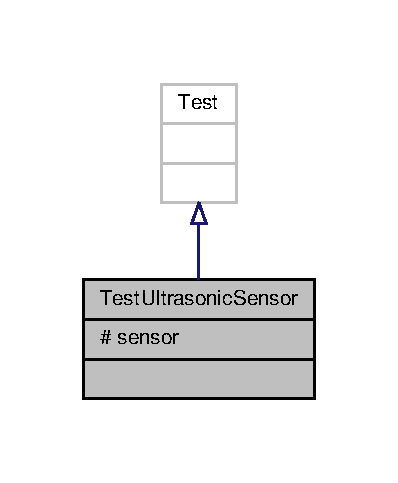
\includegraphics[width=191pt]{class_test_ultrasonic_sensor__inherit__graph}
\end{center}
\end{figure}
\subsection*{Protected Attributes}
\begin{DoxyCompactItemize}
\item 
\hyperlink{class_ultrasonic_sensor}{Ultrasonic\+Sensor} \hyperlink{class_test_ultrasonic_sensor_abaaead54c0ad8a32f353b38b2f84127a}{sensor}
\end{DoxyCompactItemize}


\subsection{Detailed Description}
Class to test the working of Ultrasonic sensor. Create an instance of ultrasonic sensor which can be used for testing. 

Definition at line 20 of file test\+\_\+ultrasonic\+\_\+sensor.\+cpp.



\subsection{Member Data Documentation}
\index{Test\+Ultrasonic\+Sensor@{Test\+Ultrasonic\+Sensor}!sensor@{sensor}}
\index{sensor@{sensor}!Test\+Ultrasonic\+Sensor@{Test\+Ultrasonic\+Sensor}}
\subsubsection[{\texorpdfstring{sensor}{sensor}}]{\setlength{\rightskip}{0pt plus 5cm}{\bf Ultrasonic\+Sensor} Test\+Ultrasonic\+Sensor\+::sensor\hspace{0.3cm}{\ttfamily [protected]}}\hypertarget{class_test_ultrasonic_sensor_abaaead54c0ad8a32f353b38b2f84127a}{}\label{class_test_ultrasonic_sensor_abaaead54c0ad8a32f353b38b2f84127a}


Definition at line 22 of file test\+\_\+ultrasonic\+\_\+sensor.\+cpp.



The documentation for this class was generated from the following file\+:\begin{DoxyCompactItemize}
\item 
/home/nrparikh/\+Desktop/acme\+\_\+robotics\+\_\+perception\+\_\+module/test/\hyperlink{test__ultrasonic__sensor_8cpp}{test\+\_\+ultrasonic\+\_\+sensor.\+cpp}\end{DoxyCompactItemize}

\hypertarget{class_ultrasonic_sensor}{}\section{Ultrasonic\+Sensor Class Reference}
\label{class_ultrasonic_sensor}\index{Ultrasonic\+Sensor@{Ultrasonic\+Sensor}}


{\ttfamily \#include $<$ultrasonic\+\_\+sensor.\+hpp$>$}



Inheritance diagram for Ultrasonic\+Sensor\+:
\nopagebreak
\begin{figure}[H]
\begin{center}
\leavevmode
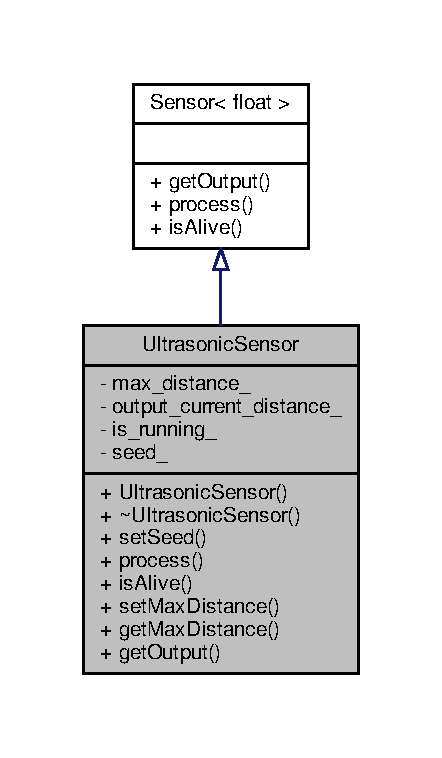
\includegraphics[width=212pt]{class_ultrasonic_sensor__inherit__graph}
\end{center}
\end{figure}
\subsection*{Public Member Functions}
\begin{DoxyCompactItemize}
\item 
\hyperlink{class_ultrasonic_sensor_afc21cb39ba75dfd008e1e82c82d2e61f}{Ultrasonic\+Sensor} ()
\begin{DoxyCompactList}\small\item\em Constructor of the class \hyperlink{class_ultrasonic_sensor}{Ultrasonic\+Sensor}. Set the is\+\_\+running\+\_\+ flag to true. \end{DoxyCompactList}\item 
\hyperlink{class_ultrasonic_sensor_aec2722048b7070bd2b0f665b210f0d1a}{$\sim$\+Ultrasonic\+Sensor} ()
\begin{DoxyCompactList}\small\item\em Destructor of the class \hyperlink{class_ultrasonic_sensor}{Ultrasonic\+Sensor}. \end{DoxyCompactList}\item 
auto \hyperlink{class_ultrasonic_sensor_abb877ee0a45cc3a1856a13536c95f474}{set\+Seed} (const int \&seed) -\/$>$ void
\begin{DoxyCompactList}\small\item\em Method to set constant seed if needed. \end{DoxyCompactList}\item 
auto \hyperlink{class_ultrasonic_sensor_af20b33a57f5b4522566d6856f6ca4428}{process} () -\/$>$ void
\begin{DoxyCompactList}\small\item\em Override the virtual method \char`\"{}process\char`\"{} of \hyperlink{class_sensor}{Sensor} class. This method takes the current distance reading and updates its reading value. \end{DoxyCompactList}\item 
auto \hyperlink{class_ultrasonic_sensor_af10dfe88aa79e9c108055d5b4b5144e9}{is\+Alive} () -\/$>$ bool
\begin{DoxyCompactList}\small\item\em Override the virtual method \char`\"{}is\+Alive\char`\"{} of \hyperlink{class_sensor}{Sensor} class. This method checks if the sensor is running or not. \end{DoxyCompactList}\item 
auto \hyperlink{class_ultrasonic_sensor_a831b3ae96fb0537d8a7e7c12e8214f66}{set\+Max\+Distance} (float max\+Dist) -\/$>$ void
\begin{DoxyCompactList}\small\item\em Method to set the max distance parameter of the class. \end{DoxyCompactList}\item 
auto \hyperlink{class_ultrasonic_sensor_af1ea4298d3ac580095e59d4b63e9076c}{get\+Max\+Distance} () -\/$>$ float
\begin{DoxyCompactList}\small\item\em Method to get the max distance parameter of the class. \end{DoxyCompactList}\item 
auto \hyperlink{class_ultrasonic_sensor_a0776a669d6c30958fe316cb2daa3e6e7}{get\+Output} () -\/$>$ float
\begin{DoxyCompactList}\small\item\em Override the method \char`\"{}get\+Output\char`\"{} of \hyperlink{class_sensor}{Sensor} class. This method returns the output value of the class which is the current distance reading taken by the sensor. \end{DoxyCompactList}\end{DoxyCompactItemize}
\subsection*{Private Attributes}
\begin{DoxyCompactItemize}
\item 
float \hyperlink{class_ultrasonic_sensor_a7a41e3e74c23db857fd6cc3728439461}{max\+\_\+distance\+\_\+}
\begin{DoxyCompactList}\small\item\em Maximum distance that can be read by the sensor. \end{DoxyCompactList}\item 
float \hyperlink{class_ultrasonic_sensor_a96a5d6ca72fcbe545ea88f504b24b44a}{output\+\_\+current\+\_\+distance\+\_\+}
\item 
bool \hyperlink{class_ultrasonic_sensor_a7d98b5005d41e9bb8fd84c71dde4079a}{is\+\_\+running\+\_\+}
\item 
unsigned int \hyperlink{class_ultrasonic_sensor_a3d7bb6ec05405169a0ea40432a79e318}{seed\+\_\+}
\end{DoxyCompactItemize}


\subsection{Detailed Description}


Definition at line 23 of file ultrasonic\+\_\+sensor.\+hpp.



\subsection{Constructor \& Destructor Documentation}
\index{Ultrasonic\+Sensor@{Ultrasonic\+Sensor}!Ultrasonic\+Sensor@{Ultrasonic\+Sensor}}
\index{Ultrasonic\+Sensor@{Ultrasonic\+Sensor}!Ultrasonic\+Sensor@{Ultrasonic\+Sensor}}
\subsubsection[{\texorpdfstring{Ultrasonic\+Sensor()}{UltrasonicSensor()}}]{\setlength{\rightskip}{0pt plus 5cm}Ultrasonic\+Sensor\+::\+Ultrasonic\+Sensor (
\begin{DoxyParamCaption}
{}
\end{DoxyParamCaption}
)}\hypertarget{class_ultrasonic_sensor_afc21cb39ba75dfd008e1e82c82d2e61f}{}\label{class_ultrasonic_sensor_afc21cb39ba75dfd008e1e82c82d2e61f}


Constructor of the class \hyperlink{class_ultrasonic_sensor}{Ultrasonic\+Sensor}. Set the is\+\_\+running\+\_\+ flag to true. 

\begin{DoxyReturn}{Returns}
void\+: Return nothing. 
\end{DoxyReturn}


Definition at line 15 of file ultra\+\_\+sensor.\+cpp.

\index{Ultrasonic\+Sensor@{Ultrasonic\+Sensor}!````~Ultrasonic\+Sensor@{$\sim$\+Ultrasonic\+Sensor}}
\index{````~Ultrasonic\+Sensor@{$\sim$\+Ultrasonic\+Sensor}!Ultrasonic\+Sensor@{Ultrasonic\+Sensor}}
\subsubsection[{\texorpdfstring{$\sim$\+Ultrasonic\+Sensor()}{~UltrasonicSensor()}}]{\setlength{\rightskip}{0pt plus 5cm}Ultrasonic\+Sensor\+::$\sim$\+Ultrasonic\+Sensor (
\begin{DoxyParamCaption}
{}
\end{DoxyParamCaption}
)}\hypertarget{class_ultrasonic_sensor_aec2722048b7070bd2b0f665b210f0d1a}{}\label{class_ultrasonic_sensor_aec2722048b7070bd2b0f665b210f0d1a}


Destructor of the class \hyperlink{class_ultrasonic_sensor}{Ultrasonic\+Sensor}. 

\begin{DoxyReturn}{Returns}
void\+: Return nothing. 
\end{DoxyReturn}


Definition at line 23 of file ultra\+\_\+sensor.\+cpp.



\subsection{Member Function Documentation}
\index{Ultrasonic\+Sensor@{Ultrasonic\+Sensor}!get\+Max\+Distance@{get\+Max\+Distance}}
\index{get\+Max\+Distance@{get\+Max\+Distance}!Ultrasonic\+Sensor@{Ultrasonic\+Sensor}}
\subsubsection[{\texorpdfstring{get\+Max\+Distance() -\/$>$ float}{getMaxDistance() -> float}}]{\setlength{\rightskip}{0pt plus 5cm}auto Ultrasonic\+Sensor\+::get\+Max\+Distance (
\begin{DoxyParamCaption}
{}
\end{DoxyParamCaption}
) -\/$>$ float}\hypertarget{class_ultrasonic_sensor_af1ea4298d3ac580095e59d4b63e9076c}{}\label{class_ultrasonic_sensor_af1ea4298d3ac580095e59d4b63e9076c}


Method to get the max distance parameter of the class. 

\begin{DoxyReturn}{Returns}
float\+: Return the maximum distance that can be read by the sensor(max\+\_\+distance\+\_\+). 
\end{DoxyReturn}


Definition at line 51 of file ultra\+\_\+sensor.\+cpp.

\index{Ultrasonic\+Sensor@{Ultrasonic\+Sensor}!get\+Output@{get\+Output}}
\index{get\+Output@{get\+Output}!Ultrasonic\+Sensor@{Ultrasonic\+Sensor}}
\subsubsection[{\texorpdfstring{get\+Output() -\/$>$ float}{getOutput() -> float}}]{\setlength{\rightskip}{0pt plus 5cm}auto Ultrasonic\+Sensor\+::get\+Output (
\begin{DoxyParamCaption}
{}
\end{DoxyParamCaption}
) -\/$>$ float\hspace{0.3cm}{\ttfamily [virtual]}}\hypertarget{class_ultrasonic_sensor_a0776a669d6c30958fe316cb2daa3e6e7}{}\label{class_ultrasonic_sensor_a0776a669d6c30958fe316cb2daa3e6e7}


Override the method \char`\"{}get\+Output\char`\"{} of \hyperlink{class_sensor}{Sensor} class. This method returns the output value of the class which is the current distance reading taken by the sensor. 

\begin{DoxyReturn}{Returns}
float\+: Return the current distance read by the sensor(output\+\_\+current\+\_\+distance\+\_\+). 
\end{DoxyReturn}


Implements \hyperlink{class_sensor_abdc2eb130cb935cb090470d1fe6cc499}{Sensor$<$ float $>$}.



Definition at line 55 of file ultra\+\_\+sensor.\+cpp.

\index{Ultrasonic\+Sensor@{Ultrasonic\+Sensor}!is\+Alive@{is\+Alive}}
\index{is\+Alive@{is\+Alive}!Ultrasonic\+Sensor@{Ultrasonic\+Sensor}}
\subsubsection[{\texorpdfstring{is\+Alive() -\/$>$ bool}{isAlive() -> bool}}]{\setlength{\rightskip}{0pt plus 5cm}auto Ultrasonic\+Sensor\+::is\+Alive (
\begin{DoxyParamCaption}
{}
\end{DoxyParamCaption}
) -\/$>$ bool\hspace{0.3cm}{\ttfamily [virtual]}}\hypertarget{class_ultrasonic_sensor_af10dfe88aa79e9c108055d5b4b5144e9}{}\label{class_ultrasonic_sensor_af10dfe88aa79e9c108055d5b4b5144e9}


Override the virtual method \char`\"{}is\+Alive\char`\"{} of \hyperlink{class_sensor}{Sensor} class. This method checks if the sensor is running or not. 

\begin{DoxyReturn}{Returns}
bool\+: Return \char`\"{}true\char`\"{} if the sensor is running, \char`\"{}false\char`\"{} otherwise. 
\end{DoxyReturn}


Implements \hyperlink{class_sensor_a7ae0a8c02805d3b2b8306d01da2a2db8}{Sensor$<$ float $>$}.



Definition at line 43 of file ultra\+\_\+sensor.\+cpp.

\index{Ultrasonic\+Sensor@{Ultrasonic\+Sensor}!process@{process}}
\index{process@{process}!Ultrasonic\+Sensor@{Ultrasonic\+Sensor}}
\subsubsection[{\texorpdfstring{process() -\/$>$ void}{process() -> void}}]{\setlength{\rightskip}{0pt plus 5cm}auto Ultrasonic\+Sensor\+::process (
\begin{DoxyParamCaption}
{}
\end{DoxyParamCaption}
) -\/$>$ void}\hypertarget{class_ultrasonic_sensor_af20b33a57f5b4522566d6856f6ca4428}{}\label{class_ultrasonic_sensor_af20b33a57f5b4522566d6856f6ca4428}


Override the virtual method \char`\"{}process\char`\"{} of \hyperlink{class_sensor}{Sensor} class. This method takes the current distance reading and updates its reading value. 

\begin{DoxyReturn}{Returns}
void\+: Return nothing 
\end{DoxyReturn}


Definition at line 29 of file ultra\+\_\+sensor.\+cpp.

\index{Ultrasonic\+Sensor@{Ultrasonic\+Sensor}!set\+Max\+Distance@{set\+Max\+Distance}}
\index{set\+Max\+Distance@{set\+Max\+Distance}!Ultrasonic\+Sensor@{Ultrasonic\+Sensor}}
\subsubsection[{\texorpdfstring{set\+Max\+Distance(float max\+Dist) -\/$>$ void}{setMaxDistance(float maxDist) -> void}}]{\setlength{\rightskip}{0pt plus 5cm}auto Ultrasonic\+Sensor\+::set\+Max\+Distance (
\begin{DoxyParamCaption}
\item[{float}]{max\+Dist}
\end{DoxyParamCaption}
) -\/$>$ void}\hypertarget{class_ultrasonic_sensor_a831b3ae96fb0537d8a7e7c12e8214f66}{}\label{class_ultrasonic_sensor_a831b3ae96fb0537d8a7e7c12e8214f66}


Method to set the max distance parameter of the class. 


\begin{DoxyParams}{Parameters}
{\em max\+Dist} & Pass the value which is set to be as maximum distance\\
\hline
\end{DoxyParams}
\begin{DoxyReturn}{Returns}
void\+: Return nothing. 
\end{DoxyReturn}


Definition at line 47 of file ultra\+\_\+sensor.\+cpp.

\index{Ultrasonic\+Sensor@{Ultrasonic\+Sensor}!set\+Seed@{set\+Seed}}
\index{set\+Seed@{set\+Seed}!Ultrasonic\+Sensor@{Ultrasonic\+Sensor}}
\subsubsection[{\texorpdfstring{set\+Seed(const int \&seed) -\/$>$ void}{setSeed(const int &seed) -> void}}]{\setlength{\rightskip}{0pt plus 5cm}auto Ultrasonic\+Sensor\+::set\+Seed (
\begin{DoxyParamCaption}
\item[{const int \&}]{seed}
\end{DoxyParamCaption}
) -\/$>$ void}\hypertarget{class_ultrasonic_sensor_abb877ee0a45cc3a1856a13536c95f474}{}\label{class_ultrasonic_sensor_abb877ee0a45cc3a1856a13536c95f474}


Method to set constant seed if needed. 


\begin{DoxyParams}[1]{Parameters}
\mbox{\tt in}  & {\em seed} & Constant value to be set as seed\\
\hline
\end{DoxyParams}
\begin{DoxyReturn}{Returns}
void\+: Return nothing 
\end{DoxyReturn}


Definition at line 25 of file ultra\+\_\+sensor.\+cpp.



\subsection{Member Data Documentation}
\index{Ultrasonic\+Sensor@{Ultrasonic\+Sensor}!is\+\_\+running\+\_\+@{is\+\_\+running\+\_\+}}
\index{is\+\_\+running\+\_\+@{is\+\_\+running\+\_\+}!Ultrasonic\+Sensor@{Ultrasonic\+Sensor}}
\subsubsection[{\texorpdfstring{is\+\_\+running\+\_\+}{is_running_}}]{\setlength{\rightskip}{0pt plus 5cm}bool Ultrasonic\+Sensor\+::is\+\_\+running\+\_\+\hspace{0.3cm}{\ttfamily [private]}}\hypertarget{class_ultrasonic_sensor_a7d98b5005d41e9bb8fd84c71dde4079a}{}\label{class_ultrasonic_sensor_a7d98b5005d41e9bb8fd84c71dde4079a}
Flag to test if the ultrasonic sensor is running or not. 

Definition at line 89 of file ultrasonic\+\_\+sensor.\+hpp.

\index{Ultrasonic\+Sensor@{Ultrasonic\+Sensor}!max\+\_\+distance\+\_\+@{max\+\_\+distance\+\_\+}}
\index{max\+\_\+distance\+\_\+@{max\+\_\+distance\+\_\+}!Ultrasonic\+Sensor@{Ultrasonic\+Sensor}}
\subsubsection[{\texorpdfstring{max\+\_\+distance\+\_\+}{max_distance_}}]{\setlength{\rightskip}{0pt plus 5cm}float Ultrasonic\+Sensor\+::max\+\_\+distance\+\_\+\hspace{0.3cm}{\ttfamily [private]}}\hypertarget{class_ultrasonic_sensor_a7a41e3e74c23db857fd6cc3728439461}{}\label{class_ultrasonic_sensor_a7a41e3e74c23db857fd6cc3728439461}


Maximum distance that can be read by the sensor. 



Definition at line 86 of file ultrasonic\+\_\+sensor.\+hpp.

\index{Ultrasonic\+Sensor@{Ultrasonic\+Sensor}!output\+\_\+current\+\_\+distance\+\_\+@{output\+\_\+current\+\_\+distance\+\_\+}}
\index{output\+\_\+current\+\_\+distance\+\_\+@{output\+\_\+current\+\_\+distance\+\_\+}!Ultrasonic\+Sensor@{Ultrasonic\+Sensor}}
\subsubsection[{\texorpdfstring{output\+\_\+current\+\_\+distance\+\_\+}{output_current_distance_}}]{\setlength{\rightskip}{0pt plus 5cm}float Ultrasonic\+Sensor\+::output\+\_\+current\+\_\+distance\+\_\+\hspace{0.3cm}{\ttfamily [private]}}\hypertarget{class_ultrasonic_sensor_a96a5d6ca72fcbe545ea88f504b24b44a}{}\label{class_ultrasonic_sensor_a96a5d6ca72fcbe545ea88f504b24b44a}
Current distance reading. Output of the class. 

Definition at line 87 of file ultrasonic\+\_\+sensor.\+hpp.

\index{Ultrasonic\+Sensor@{Ultrasonic\+Sensor}!seed\+\_\+@{seed\+\_\+}}
\index{seed\+\_\+@{seed\+\_\+}!Ultrasonic\+Sensor@{Ultrasonic\+Sensor}}
\subsubsection[{\texorpdfstring{seed\+\_\+}{seed_}}]{\setlength{\rightskip}{0pt plus 5cm}unsigned int Ultrasonic\+Sensor\+::seed\+\_\+\hspace{0.3cm}{\ttfamily [private]}}\hypertarget{class_ultrasonic_sensor_a3d7bb6ec05405169a0ea40432a79e318}{}\label{class_ultrasonic_sensor_a3d7bb6ec05405169a0ea40432a79e318}


Definition at line 91 of file ultrasonic\+\_\+sensor.\+hpp.



The documentation for this class was generated from the following files\+:\begin{DoxyCompactItemize}
\item 
/home/nrparikh/\+Desktop/acme\+\_\+robotics\+\_\+perception\+\_\+module/include/\hyperlink{ultrasonic__sensor_8hpp}{ultrasonic\+\_\+sensor.\+hpp}\item 
/home/nrparikh/\+Desktop/acme\+\_\+robotics\+\_\+perception\+\_\+module/app/\hyperlink{ultra__sensor_8cpp}{ultra\+\_\+sensor.\+cpp}\end{DoxyCompactItemize}

\chapter{File Documentation}
\hypertarget{_8ycm__extra__conf_8py}{}\section{/home/nrparikh/acme\+\_\+robotics\+\_\+perception\+\_\+module/.ycm\+\_\+extra\+\_\+conf.\+py File Reference}
\label{_8ycm__extra__conf_8py}\index{/home/nrparikh/acme\+\_\+robotics\+\_\+perception\+\_\+module/.\+ycm\+\_\+extra\+\_\+conf.\+py@{/home/nrparikh/acme\+\_\+robotics\+\_\+perception\+\_\+module/.\+ycm\+\_\+extra\+\_\+conf.\+py}}
\subsection*{Functions}
\begin{DoxyCompactItemize}
\item 
def \hyperlink{_8ycm__extra__conf_8py_aab283cdb607efa6a1a7aaa3f089c63f1}{Directory\+Of\+This\+Script} ()
\item 
def \hyperlink{_8ycm__extra__conf_8py_aa20d30f8cc08fc0ab076b4cf458e0d3d}{Make\+Relative\+Paths\+In\+Flags\+Absolute} (\hyperlink{_8ycm__extra__conf_8py_abd73d8e4551f1a637280b3876d1ae2e3}{flags}, working\+\_\+directory)
\item 
def \hyperlink{_8ycm__extra__conf_8py_a6bb59f541be0dcbde53eba606d48ddf8}{Is\+Header\+File} (filename)
\item 
def \hyperlink{_8ycm__extra__conf_8py_a42a14573593ce75cd6e385a85326111f}{Get\+Compilation\+Info\+For\+File} (filename)
\item 
def \hyperlink{_8ycm__extra__conf_8py_a51f8bcdc9a3b791e6a88d798e6c786b3}{Flags\+For\+File} (filename, kwargs)
\end{DoxyCompactItemize}
\subsection*{Variables}
\begin{DoxyCompactItemize}
\item 
list \hyperlink{_8ycm__extra__conf_8py_abd73d8e4551f1a637280b3876d1ae2e3}{flags}
\item 
string \hyperlink{_8ycm__extra__conf_8py_a6a4d7e96c7bc9093b406af626b7936a2}{compilation\+\_\+database\+\_\+folder} = \textquotesingle{}\textquotesingle{}
\item 
\hyperlink{_8ycm__extra__conf_8py_a64dbaa3229ec575b68ec333442e10cee}{database} = ycm\+\_\+core.\+Compilation\+Database( \hyperlink{_8ycm__extra__conf_8py_a6a4d7e96c7bc9093b406af626b7936a2}{compilation\+\_\+database\+\_\+folder} )
\item 
list \hyperlink{_8ycm__extra__conf_8py_a47014996e1e517071cd0412a22adb123}{S\+O\+U\+R\+C\+E\+\_\+\+E\+X\+T\+E\+N\+S\+I\+O\+NS} = \mbox{[} \textquotesingle{}.C\textquotesingle{}, \textquotesingle{}.cpp\textquotesingle{}, \textquotesingle{}.cxx\textquotesingle{}, \textquotesingle{}.cc\textquotesingle{}, \textquotesingle{}.c\textquotesingle{}, \textquotesingle{}.m\textquotesingle{}, \textquotesingle{}.mm\textquotesingle{} \mbox{]}
\end{DoxyCompactItemize}


\subsection{Function Documentation}
\index{.\+ycm\+\_\+extra\+\_\+conf.\+py@{.\+ycm\+\_\+extra\+\_\+conf.\+py}!Directory\+Of\+This\+Script@{Directory\+Of\+This\+Script}}
\index{Directory\+Of\+This\+Script@{Directory\+Of\+This\+Script}!.\+ycm\+\_\+extra\+\_\+conf.\+py@{.\+ycm\+\_\+extra\+\_\+conf.\+py}}
\subsubsection[{\texorpdfstring{Directory\+Of\+This\+Script()}{DirectoryOfThisScript()}}]{\setlength{\rightskip}{0pt plus 5cm}def Directory\+Of\+This\+Script (
\begin{DoxyParamCaption}
{}
\end{DoxyParamCaption}
)}\hypertarget{_8ycm__extra__conf_8py_aab283cdb607efa6a1a7aaa3f089c63f1}{}\label{_8ycm__extra__conf_8py_aab283cdb607efa6a1a7aaa3f089c63f1}


Definition at line 71 of file .\+ycm\+\_\+extra\+\_\+conf.\+py.

\index{.\+ycm\+\_\+extra\+\_\+conf.\+py@{.\+ycm\+\_\+extra\+\_\+conf.\+py}!Flags\+For\+File@{Flags\+For\+File}}
\index{Flags\+For\+File@{Flags\+For\+File}!.\+ycm\+\_\+extra\+\_\+conf.\+py@{.\+ycm\+\_\+extra\+\_\+conf.\+py}}
\subsubsection[{\texorpdfstring{Flags\+For\+File(filename, kwargs)}{FlagsForFile(filename, kwargs)}}]{\setlength{\rightskip}{0pt plus 5cm}def Flags\+For\+File (
\begin{DoxyParamCaption}
\item[{}]{filename, }
\item[{}]{kwargs}
\end{DoxyParamCaption}
)}\hypertarget{_8ycm__extra__conf_8py_a51f8bcdc9a3b791e6a88d798e6c786b3}{}\label{_8ycm__extra__conf_8py_a51f8bcdc9a3b791e6a88d798e6c786b3}


Definition at line 127 of file .\+ycm\+\_\+extra\+\_\+conf.\+py.

\index{.\+ycm\+\_\+extra\+\_\+conf.\+py@{.\+ycm\+\_\+extra\+\_\+conf.\+py}!Get\+Compilation\+Info\+For\+File@{Get\+Compilation\+Info\+For\+File}}
\index{Get\+Compilation\+Info\+For\+File@{Get\+Compilation\+Info\+For\+File}!.\+ycm\+\_\+extra\+\_\+conf.\+py@{.\+ycm\+\_\+extra\+\_\+conf.\+py}}
\subsubsection[{\texorpdfstring{Get\+Compilation\+Info\+For\+File(filename)}{GetCompilationInfoForFile(filename)}}]{\setlength{\rightskip}{0pt plus 5cm}def Get\+Compilation\+Info\+For\+File (
\begin{DoxyParamCaption}
\item[{}]{filename}
\end{DoxyParamCaption}
)}\hypertarget{_8ycm__extra__conf_8py_a42a14573593ce75cd6e385a85326111f}{}\label{_8ycm__extra__conf_8py_a42a14573593ce75cd6e385a85326111f}


Definition at line 109 of file .\+ycm\+\_\+extra\+\_\+conf.\+py.

\index{.\+ycm\+\_\+extra\+\_\+conf.\+py@{.\+ycm\+\_\+extra\+\_\+conf.\+py}!Is\+Header\+File@{Is\+Header\+File}}
\index{Is\+Header\+File@{Is\+Header\+File}!.\+ycm\+\_\+extra\+\_\+conf.\+py@{.\+ycm\+\_\+extra\+\_\+conf.\+py}}
\subsubsection[{\texorpdfstring{Is\+Header\+File(filename)}{IsHeaderFile(filename)}}]{\setlength{\rightskip}{0pt plus 5cm}def Is\+Header\+File (
\begin{DoxyParamCaption}
\item[{}]{filename}
\end{DoxyParamCaption}
)}\hypertarget{_8ycm__extra__conf_8py_a6bb59f541be0dcbde53eba606d48ddf8}{}\label{_8ycm__extra__conf_8py_a6bb59f541be0dcbde53eba606d48ddf8}


Definition at line 104 of file .\+ycm\+\_\+extra\+\_\+conf.\+py.

\index{.\+ycm\+\_\+extra\+\_\+conf.\+py@{.\+ycm\+\_\+extra\+\_\+conf.\+py}!Make\+Relative\+Paths\+In\+Flags\+Absolute@{Make\+Relative\+Paths\+In\+Flags\+Absolute}}
\index{Make\+Relative\+Paths\+In\+Flags\+Absolute@{Make\+Relative\+Paths\+In\+Flags\+Absolute}!.\+ycm\+\_\+extra\+\_\+conf.\+py@{.\+ycm\+\_\+extra\+\_\+conf.\+py}}
\subsubsection[{\texorpdfstring{Make\+Relative\+Paths\+In\+Flags\+Absolute(flags, working\+\_\+directory)}{MakeRelativePathsInFlagsAbsolute(flags, working_directory)}}]{\setlength{\rightskip}{0pt plus 5cm}def Make\+Relative\+Paths\+In\+Flags\+Absolute (
\begin{DoxyParamCaption}
\item[{}]{flags, }
\item[{}]{working\+\_\+directory}
\end{DoxyParamCaption}
)}\hypertarget{_8ycm__extra__conf_8py_aa20d30f8cc08fc0ab076b4cf458e0d3d}{}\label{_8ycm__extra__conf_8py_aa20d30f8cc08fc0ab076b4cf458e0d3d}


Definition at line 75 of file .\+ycm\+\_\+extra\+\_\+conf.\+py.



\subsection{Variable Documentation}
\index{.\+ycm\+\_\+extra\+\_\+conf.\+py@{.\+ycm\+\_\+extra\+\_\+conf.\+py}!compilation\+\_\+database\+\_\+folder@{compilation\+\_\+database\+\_\+folder}}
\index{compilation\+\_\+database\+\_\+folder@{compilation\+\_\+database\+\_\+folder}!.\+ycm\+\_\+extra\+\_\+conf.\+py@{.\+ycm\+\_\+extra\+\_\+conf.\+py}}
\subsubsection[{\texorpdfstring{compilation\+\_\+database\+\_\+folder}{compilation_database_folder}}]{\setlength{\rightskip}{0pt plus 5cm}string compilation\+\_\+database\+\_\+folder = \textquotesingle{}\textquotesingle{}}\hypertarget{_8ycm__extra__conf_8py_a6a4d7e96c7bc9093b406af626b7936a2}{}\label{_8ycm__extra__conf_8py_a6a4d7e96c7bc9093b406af626b7936a2}


Definition at line 62 of file .\+ycm\+\_\+extra\+\_\+conf.\+py.

\index{.\+ycm\+\_\+extra\+\_\+conf.\+py@{.\+ycm\+\_\+extra\+\_\+conf.\+py}!database@{database}}
\index{database@{database}!.\+ycm\+\_\+extra\+\_\+conf.\+py@{.\+ycm\+\_\+extra\+\_\+conf.\+py}}
\subsubsection[{\texorpdfstring{database}{database}}]{\setlength{\rightskip}{0pt plus 5cm}database = ycm\+\_\+core.\+Compilation\+Database( {\bf compilation\+\_\+database\+\_\+folder} )}\hypertarget{_8ycm__extra__conf_8py_a64dbaa3229ec575b68ec333442e10cee}{}\label{_8ycm__extra__conf_8py_a64dbaa3229ec575b68ec333442e10cee}


Definition at line 65 of file .\+ycm\+\_\+extra\+\_\+conf.\+py.

\index{.\+ycm\+\_\+extra\+\_\+conf.\+py@{.\+ycm\+\_\+extra\+\_\+conf.\+py}!flags@{flags}}
\index{flags@{flags}!.\+ycm\+\_\+extra\+\_\+conf.\+py@{.\+ycm\+\_\+extra\+\_\+conf.\+py}}
\subsubsection[{\texorpdfstring{flags}{flags}}]{\setlength{\rightskip}{0pt plus 5cm}list flags}\hypertarget{_8ycm__extra__conf_8py_abd73d8e4551f1a637280b3876d1ae2e3}{}\label{_8ycm__extra__conf_8py_abd73d8e4551f1a637280b3876d1ae2e3}
{\bfseries Initial value\+:}
\begin{DoxyCode}
1 = [
2     \textcolor{stringliteral}{'-x'},
3     \textcolor{stringliteral}{'c++'},
4     \textcolor{stringliteral}{'-DGTEST\_HAS\_PTHREAD=1'},
5     \textcolor{stringliteral}{'-I/Users/david/code/scratch/cpp/include'},
6     \textcolor{stringliteral}{'-I/Users/david/code/scratch/cpp/test/../vendor/googletest/googletest/include'},
7     \textcolor{stringliteral}{'-I/Users/david/code/scratch/cpp/vendor/boost'},
8     \textcolor{stringliteral}{'-I/Users/david/code/scratch/cpp/vendor/googletest/googletest'},
9     \textcolor{stringliteral}{'-I/Users/david/code/scratch/cpp/vendor/googletest/googletest/include'},
10     \textcolor{stringliteral}{'-Wall'},
11     \textcolor{stringliteral}{'-Wextra'},
12     \textcolor{stringliteral}{'-Wpedantic'},
13     \textcolor{stringliteral}{'-std=c++14'},
14 ]
\end{DoxyCode}


Definition at line 36 of file .\+ycm\+\_\+extra\+\_\+conf.\+py.

\index{.\+ycm\+\_\+extra\+\_\+conf.\+py@{.\+ycm\+\_\+extra\+\_\+conf.\+py}!S\+O\+U\+R\+C\+E\+\_\+\+E\+X\+T\+E\+N\+S\+I\+O\+NS@{S\+O\+U\+R\+C\+E\+\_\+\+E\+X\+T\+E\+N\+S\+I\+O\+NS}}
\index{S\+O\+U\+R\+C\+E\+\_\+\+E\+X\+T\+E\+N\+S\+I\+O\+NS@{S\+O\+U\+R\+C\+E\+\_\+\+E\+X\+T\+E\+N\+S\+I\+O\+NS}!.\+ycm\+\_\+extra\+\_\+conf.\+py@{.\+ycm\+\_\+extra\+\_\+conf.\+py}}
\subsubsection[{\texorpdfstring{S\+O\+U\+R\+C\+E\+\_\+\+E\+X\+T\+E\+N\+S\+I\+O\+NS}{SOURCE_EXTENSIONS}}]{\setlength{\rightskip}{0pt plus 5cm}list S\+O\+U\+R\+C\+E\+\_\+\+E\+X\+T\+E\+N\+S\+I\+O\+NS = \mbox{[} \textquotesingle{}.C\textquotesingle{}, \textquotesingle{}.cpp\textquotesingle{}, \textquotesingle{}.cxx\textquotesingle{}, \textquotesingle{}.cc\textquotesingle{}, \textquotesingle{}.c\textquotesingle{}, \textquotesingle{}.m\textquotesingle{}, \textquotesingle{}.mm\textquotesingle{} \mbox{]}}\hypertarget{_8ycm__extra__conf_8py_a47014996e1e517071cd0412a22adb123}{}\label{_8ycm__extra__conf_8py_a47014996e1e517071cd0412a22adb123}


Definition at line 69 of file .\+ycm\+\_\+extra\+\_\+conf.\+py.


\hypertarget{camera_8cpp}{}\section{/home/nrparikh/acme\+\_\+robotics\+\_\+perception\+\_\+module/app/camera.cpp File Reference}
\label{camera_8cpp}\index{/home/nrparikh/acme\+\_\+robotics\+\_\+perception\+\_\+module/app/camera.\+cpp@{/home/nrparikh/acme\+\_\+robotics\+\_\+perception\+\_\+module/app/camera.\+cpp}}


D\+E\+S\+C\+R\+I\+P\+T\+I\+ON Class implementation for the class \hyperlink{class_camera}{Camera}. Uncomment the D\+E\+B\+U\+G\+\_\+\+C\+A\+M\+E\+RA if you want to debug the code.  


{\ttfamily \#include \char`\"{}camera.\+hpp\char`\"{}}\\*
Include dependency graph for camera.\+cpp\+:
\nopagebreak
\begin{figure}[H]
\begin{center}
\leavevmode
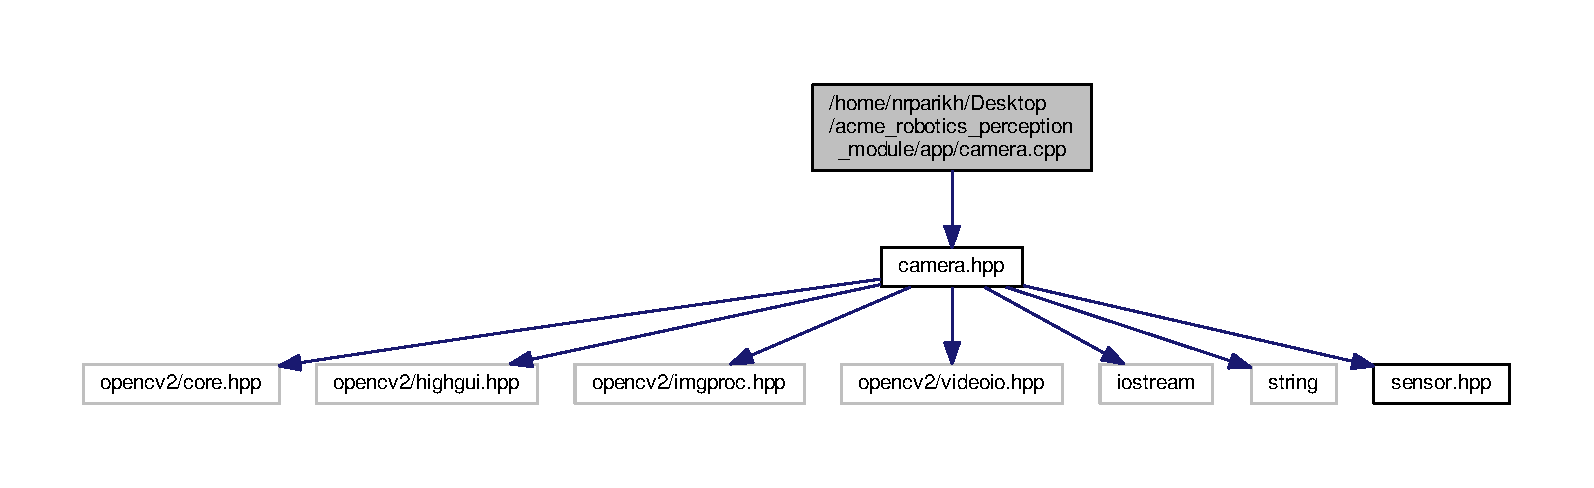
\includegraphics[width=350pt]{camera_8cpp__incl}
\end{center}
\end{figure}
\subsection*{Macros}
\begin{DoxyCompactItemize}
\item 
\#define \hyperlink{camera_8cpp_ac0543811059575e953053b2d1820d482}{D\+E\+B\+U\+G\+\_\+\+C\+A\+M\+E\+RA}
\end{DoxyCompactItemize}


\subsection{Detailed Description}
D\+E\+S\+C\+R\+I\+P\+T\+I\+ON Class implementation for the class \hyperlink{class_camera}{Camera}. Uncomment the D\+E\+B\+U\+G\+\_\+\+C\+A\+M\+E\+RA if you want to debug the code. 

\begin{DoxyAuthor}{Author}
nrparikh 
\end{DoxyAuthor}
\begin{DoxyCopyright}{Copyright}
M\+IT license 
\end{DoxyCopyright}


\subsection{Macro Definition Documentation}
\index{camera.\+cpp@{camera.\+cpp}!D\+E\+B\+U\+G\+\_\+\+C\+A\+M\+E\+RA@{D\+E\+B\+U\+G\+\_\+\+C\+A\+M\+E\+RA}}
\index{D\+E\+B\+U\+G\+\_\+\+C\+A\+M\+E\+RA@{D\+E\+B\+U\+G\+\_\+\+C\+A\+M\+E\+RA}!camera.\+cpp@{camera.\+cpp}}
\subsubsection[{\texorpdfstring{D\+E\+B\+U\+G\+\_\+\+C\+A\+M\+E\+RA}{DEBUG_CAMERA}}]{\setlength{\rightskip}{0pt plus 5cm}\#define D\+E\+B\+U\+G\+\_\+\+C\+A\+M\+E\+RA}\hypertarget{camera_8cpp_ac0543811059575e953053b2d1820d482}{}\label{camera_8cpp_ac0543811059575e953053b2d1820d482}


Definition at line 14 of file camera.\+cpp.


\hypertarget{control__module_8cpp}{}\section{/home/nrparikh/acme\+\_\+robotics\+\_\+perception\+\_\+module/app/control\+\_\+module.cpp File Reference}
\label{control__module_8cpp}\index{/home/nrparikh/acme\+\_\+robotics\+\_\+perception\+\_\+module/app/control\+\_\+module.\+cpp@{/home/nrparikh/acme\+\_\+robotics\+\_\+perception\+\_\+module/app/control\+\_\+module.\+cpp}}


D\+E\+S\+C\+R\+I\+P\+T\+I\+ON Implementation file for the class \hyperlink{class_control_module}{Control\+Module}. The class computes the action based on the readings from camera and ultrasonic sensor.  


{\ttfamily \#include \char`\"{}control\+\_\+module.\+hpp\char`\"{}}\\*
{\ttfamily \#include $<$memory$>$}\\*
{\ttfamily \#include $<$string$>$}\\*
{\ttfamily \#include $<$utility$>$}\\*
{\ttfamily \#include $<$vector$>$}\\*
Include dependency graph for control\+\_\+module.\+cpp\+:
\nopagebreak
\begin{figure}[H]
\begin{center}
\leavevmode
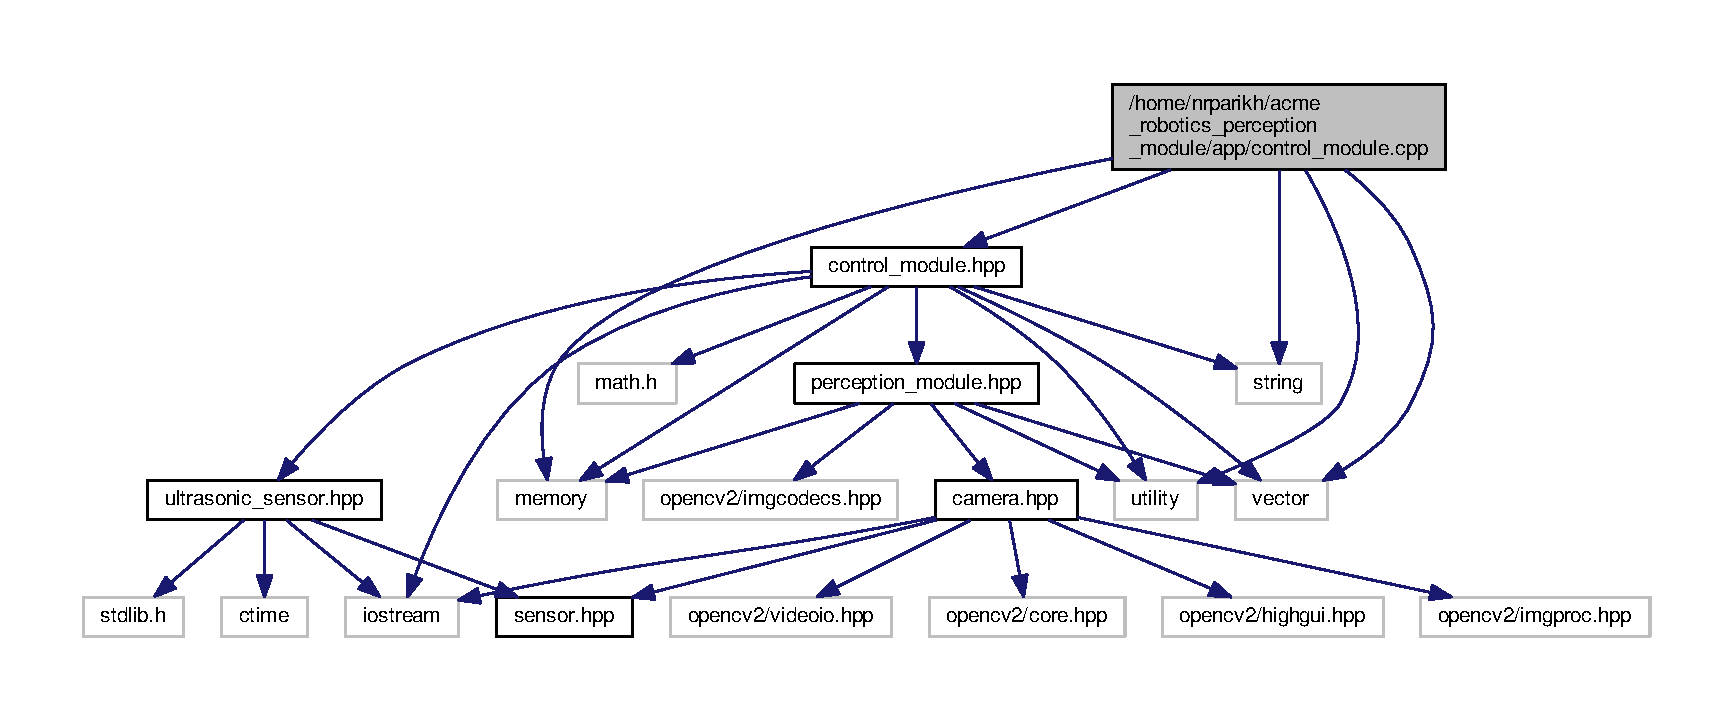
\includegraphics[width=350pt]{control__module_8cpp__incl}
\end{center}
\end{figure}
\subsection*{Macros}
\begin{DoxyCompactItemize}
\item 
\#define \hyperlink{control__module_8cpp_a5040320de72493b68d04c64242c73035}{C\+O\+N\+T\+R\+O\+L\+\_\+\+M\+O\+D\+U\+L\+E\+\_\+\+U\+S\+E\+\_\+\+L\+I\+N\+E\+\_\+\+P\+TS}
\end{DoxyCompactItemize}


\subsection{Detailed Description}
D\+E\+S\+C\+R\+I\+P\+T\+I\+ON Implementation file for the class \hyperlink{class_control_module}{Control\+Module}. The class computes the action based on the readings from camera and ultrasonic sensor. 

\begin{DoxyAuthor}{Author}
nrparikh 
\end{DoxyAuthor}
\begin{DoxyCopyright}{Copyright}
M\+IT license 
\end{DoxyCopyright}


\subsection{Macro Definition Documentation}
\index{control\+\_\+module.\+cpp@{control\+\_\+module.\+cpp}!C\+O\+N\+T\+R\+O\+L\+\_\+\+M\+O\+D\+U\+L\+E\+\_\+\+U\+S\+E\+\_\+\+L\+I\+N\+E\+\_\+\+P\+TS@{C\+O\+N\+T\+R\+O\+L\+\_\+\+M\+O\+D\+U\+L\+E\+\_\+\+U\+S\+E\+\_\+\+L\+I\+N\+E\+\_\+\+P\+TS}}
\index{C\+O\+N\+T\+R\+O\+L\+\_\+\+M\+O\+D\+U\+L\+E\+\_\+\+U\+S\+E\+\_\+\+L\+I\+N\+E\+\_\+\+P\+TS@{C\+O\+N\+T\+R\+O\+L\+\_\+\+M\+O\+D\+U\+L\+E\+\_\+\+U\+S\+E\+\_\+\+L\+I\+N\+E\+\_\+\+P\+TS}!control\+\_\+module.\+cpp@{control\+\_\+module.\+cpp}}
\subsubsection[{\texorpdfstring{C\+O\+N\+T\+R\+O\+L\+\_\+\+M\+O\+D\+U\+L\+E\+\_\+\+U\+S\+E\+\_\+\+L\+I\+N\+E\+\_\+\+P\+TS}{CONTROL_MODULE_USE_LINE_PTS}}]{\setlength{\rightskip}{0pt plus 5cm}\#define C\+O\+N\+T\+R\+O\+L\+\_\+\+M\+O\+D\+U\+L\+E\+\_\+\+U\+S\+E\+\_\+\+L\+I\+N\+E\+\_\+\+P\+TS}\hypertarget{control__module_8cpp_a5040320de72493b68d04c64242c73035}{}\label{control__module_8cpp_a5040320de72493b68d04c64242c73035}


Definition at line 18 of file control\+\_\+module.\+cpp.


\hypertarget{app_2main_8cpp}{}\section{/home/nrparikh/\+Desktop/acme\+\_\+robotics\+\_\+perception\+\_\+module/app/main.cpp File Reference}
\label{app_2main_8cpp}\index{/home/nrparikh/\+Desktop/acme\+\_\+robotics\+\_\+perception\+\_\+module/app/main.\+cpp@{/home/nrparikh/\+Desktop/acme\+\_\+robotics\+\_\+perception\+\_\+module/app/main.\+cpp}}
{\ttfamily \#include $<$string$>$}\\*
{\ttfamily \#include $<$utility$>$}\\*
{\ttfamily \#include \char`\"{}control\+\_\+module.\+hpp\char`\"{}}\\*
Include dependency graph for main.\+cpp\+:
\nopagebreak
\begin{figure}[H]
\begin{center}
\leavevmode
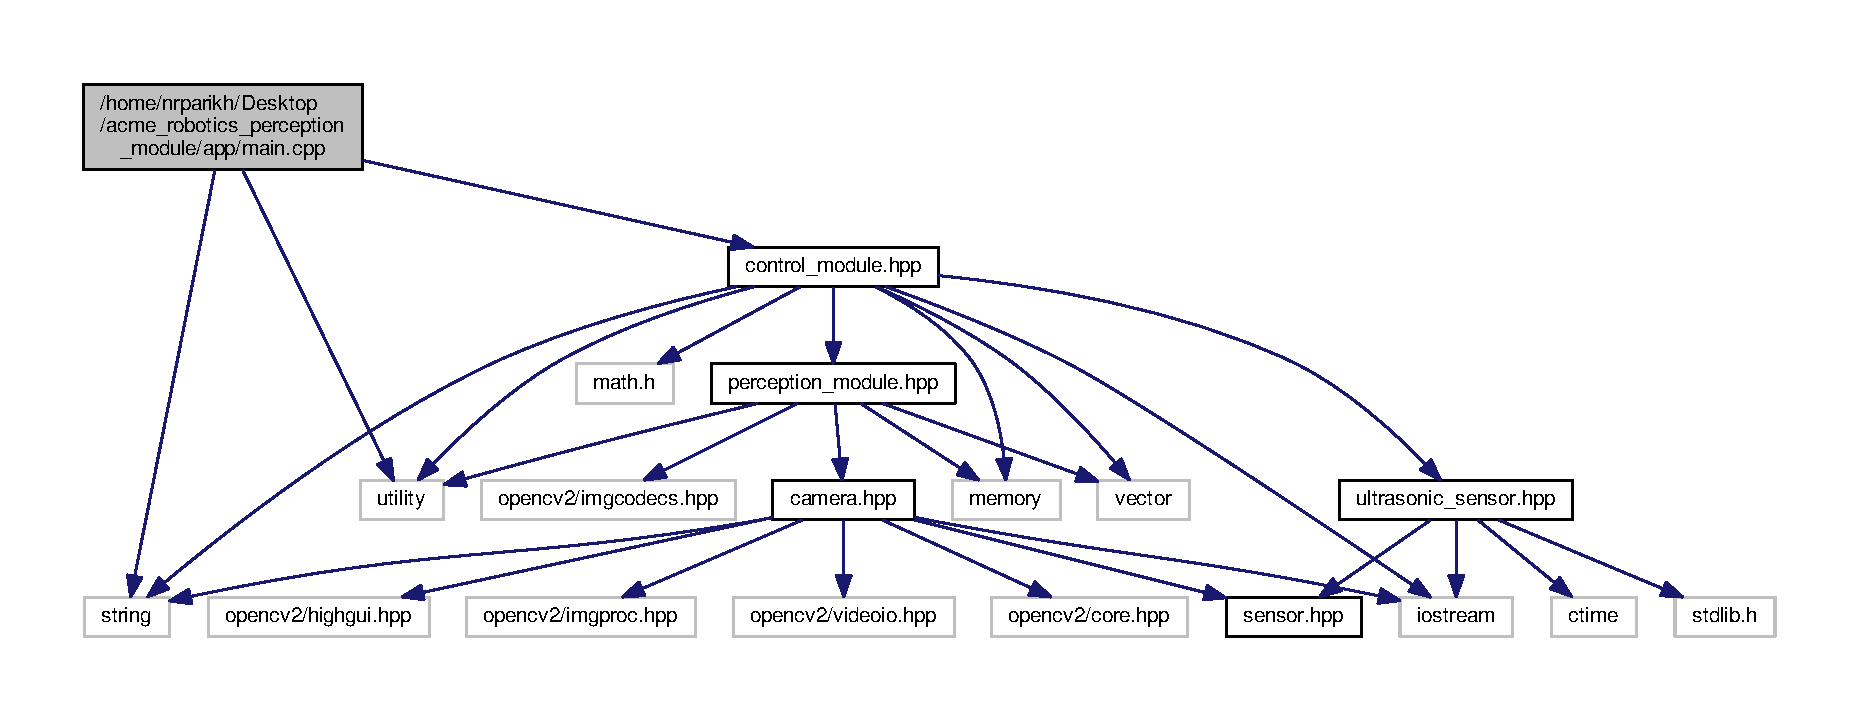
\includegraphics[width=350pt]{app_2main_8cpp__incl}
\end{center}
\end{figure}
\subsection*{Functions}
\begin{DoxyCompactItemize}
\item 
int \hyperlink{app_2main_8cpp_a0ddf1224851353fc92bfbff6f499fa97}{main} (int argc, char $\ast$argv\mbox{[}$\,$\mbox{]})
\end{DoxyCompactItemize}


\subsection{Function Documentation}
\index{app/main.\+cpp@{app/main.\+cpp}!main@{main}}
\index{main@{main}!app/main.\+cpp@{app/main.\+cpp}}
\subsubsection[{\texorpdfstring{main(int argc, char $\ast$argv[])}{main(int argc, char *argv[])}}]{\setlength{\rightskip}{0pt plus 5cm}int main (
\begin{DoxyParamCaption}
\item[{int}]{argc, }
\item[{char $\ast$}]{argv\mbox{[}$\,$\mbox{]}}
\end{DoxyParamCaption}
)}\hypertarget{app_2main_8cpp_a0ddf1224851353fc92bfbff6f499fa97}{}\label{app_2main_8cpp_a0ddf1224851353fc92bfbff6f499fa97}


Definition at line 21 of file main.\+cpp.


\hypertarget{test_2main_8cpp}{}\section{/home/nrparikh/acme\+\_\+robotics\+\_\+perception\+\_\+module/test/main.cpp File Reference}
\label{test_2main_8cpp}\index{/home/nrparikh/acme\+\_\+robotics\+\_\+perception\+\_\+module/test/main.\+cpp@{/home/nrparikh/acme\+\_\+robotics\+\_\+perception\+\_\+module/test/main.\+cpp}}
{\ttfamily \#include $<$gtest/gtest.\+h$>$}\\*
Include dependency graph for main.\+cpp\+:
\nopagebreak
\begin{figure}[H]
\begin{center}
\leavevmode
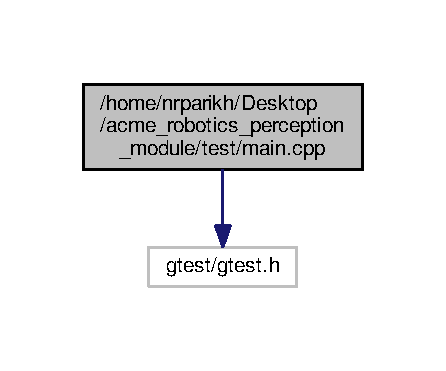
\includegraphics[width=196pt]{test_2main_8cpp__incl}
\end{center}
\end{figure}
\subsection*{Functions}
\begin{DoxyCompactItemize}
\item 
int \hyperlink{test_2main_8cpp_a3c04138a5bfe5d72780bb7e82a18e627}{main} (int argc, char $\ast$$\ast$argv)
\end{DoxyCompactItemize}


\subsection{Function Documentation}
\index{test/main.\+cpp@{test/main.\+cpp}!main@{main}}
\index{main@{main}!test/main.\+cpp@{test/main.\+cpp}}
\subsubsection[{\texorpdfstring{main(int argc, char $\ast$$\ast$argv)}{main(int argc, char **argv)}}]{\setlength{\rightskip}{0pt plus 5cm}int main (
\begin{DoxyParamCaption}
\item[{int}]{argc, }
\item[{char $\ast$$\ast$}]{argv}
\end{DoxyParamCaption}
)}\hypertarget{test_2main_8cpp_a3c04138a5bfe5d72780bb7e82a18e627}{}\label{test_2main_8cpp_a3c04138a5bfe5d72780bb7e82a18e627}


Definition at line 13 of file main.\+cpp.


\hypertarget{perception__module_8cpp}{}\section{/home/nrparikh/acme\+\_\+robotics\+\_\+perception\+\_\+module/app/perception\+\_\+module.cpp File Reference}
\label{perception__module_8cpp}\index{/home/nrparikh/acme\+\_\+robotics\+\_\+perception\+\_\+module/app/perception\+\_\+module.\+cpp@{/home/nrparikh/acme\+\_\+robotics\+\_\+perception\+\_\+module/app/perception\+\_\+module.\+cpp}}


D\+E\+S\+C\+R\+I\+P\+T\+I\+ON Implementation file for the class \hyperlink{class_perception_module}{Perception\+Module}. Uncomment the D\+E\+B\+U\+G\+\_\+\+P\+E\+R\+C\+E\+P\+T\+I\+O\+N\+\_\+\+M\+O\+D\+U\+LE to debug the module.  


{\ttfamily \#include \char`\"{}perception\+\_\+module.\+hpp\char`\"{}}\\*
{\ttfamily \#include $<$math.\+h$>$}\\*
{\ttfamily \#include $<$memory$>$}\\*
{\ttfamily \#include $<$utility$>$}\\*
{\ttfamily \#include $<$vector$>$}\\*
Include dependency graph for perception\+\_\+module.\+cpp\+:
\nopagebreak
\begin{figure}[H]
\begin{center}
\leavevmode
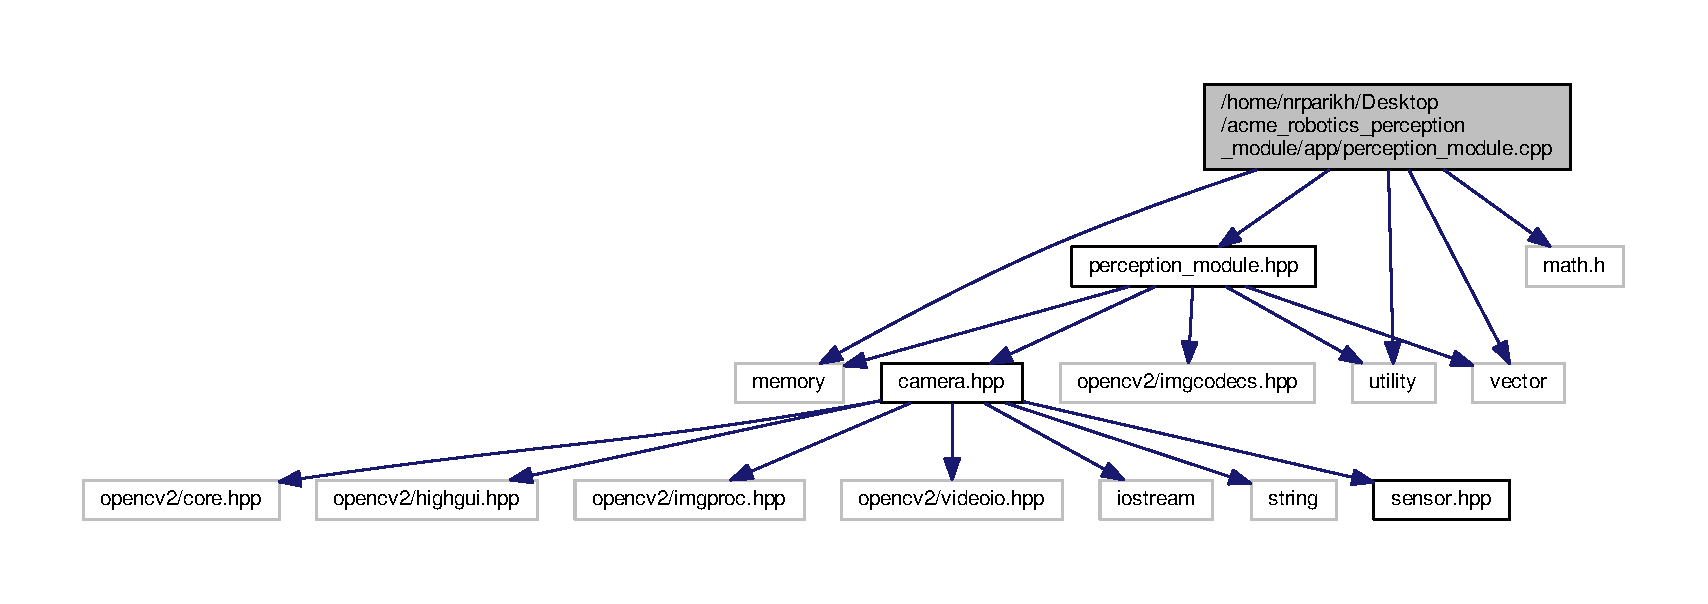
\includegraphics[width=350pt]{perception__module_8cpp__incl}
\end{center}
\end{figure}
\subsection*{Macros}
\begin{DoxyCompactItemize}
\item 
\#define \hyperlink{perception__module_8cpp_ae53f9832578a5e23f97ce875eb567bb1}{P\+E\+R\+C\+E\+P\+T\+I\+O\+N\+\_\+\+M\+O\+D\+U\+L\+E\+\_\+\+D\+E\+B\+UG}
\item 
\#define \hyperlink{perception__module_8cpp_a8efa12d50d77af44d795a4b3c50f45aa}{P\+E\+R\+C\+E\+P\+T\+I\+O\+N\+\_\+\+M\+O\+D\+U\+L\+E\+\_\+\+U\+S\+E\+\_\+\+L\+I\+N\+E\+\_\+\+P\+TS}
\end{DoxyCompactItemize}


\subsection{Detailed Description}
D\+E\+S\+C\+R\+I\+P\+T\+I\+ON Implementation file for the class \hyperlink{class_perception_module}{Perception\+Module}. Uncomment the D\+E\+B\+U\+G\+\_\+\+P\+E\+R\+C\+E\+P\+T\+I\+O\+N\+\_\+\+M\+O\+D\+U\+LE to debug the module. 

\begin{DoxyAuthor}{Author}
nrparikh 
\end{DoxyAuthor}
\begin{DoxyCopyright}{Copyright}
M\+IT license 
\end{DoxyCopyright}


\subsection{Macro Definition Documentation}
\index{perception\+\_\+module.\+cpp@{perception\+\_\+module.\+cpp}!P\+E\+R\+C\+E\+P\+T\+I\+O\+N\+\_\+\+M\+O\+D\+U\+L\+E\+\_\+\+D\+E\+B\+UG@{P\+E\+R\+C\+E\+P\+T\+I\+O\+N\+\_\+\+M\+O\+D\+U\+L\+E\+\_\+\+D\+E\+B\+UG}}
\index{P\+E\+R\+C\+E\+P\+T\+I\+O\+N\+\_\+\+M\+O\+D\+U\+L\+E\+\_\+\+D\+E\+B\+UG@{P\+E\+R\+C\+E\+P\+T\+I\+O\+N\+\_\+\+M\+O\+D\+U\+L\+E\+\_\+\+D\+E\+B\+UG}!perception\+\_\+module.\+cpp@{perception\+\_\+module.\+cpp}}
\subsubsection[{\texorpdfstring{P\+E\+R\+C\+E\+P\+T\+I\+O\+N\+\_\+\+M\+O\+D\+U\+L\+E\+\_\+\+D\+E\+B\+UG}{PERCEPTION_MODULE_DEBUG}}]{\setlength{\rightskip}{0pt plus 5cm}\#define P\+E\+R\+C\+E\+P\+T\+I\+O\+N\+\_\+\+M\+O\+D\+U\+L\+E\+\_\+\+D\+E\+B\+UG}\hypertarget{perception__module_8cpp_ae53f9832578a5e23f97ce875eb567bb1}{}\label{perception__module_8cpp_ae53f9832578a5e23f97ce875eb567bb1}


Definition at line 18 of file perception\+\_\+module.\+cpp.

\index{perception\+\_\+module.\+cpp@{perception\+\_\+module.\+cpp}!P\+E\+R\+C\+E\+P\+T\+I\+O\+N\+\_\+\+M\+O\+D\+U\+L\+E\+\_\+\+U\+S\+E\+\_\+\+L\+I\+N\+E\+\_\+\+P\+TS@{P\+E\+R\+C\+E\+P\+T\+I\+O\+N\+\_\+\+M\+O\+D\+U\+L\+E\+\_\+\+U\+S\+E\+\_\+\+L\+I\+N\+E\+\_\+\+P\+TS}}
\index{P\+E\+R\+C\+E\+P\+T\+I\+O\+N\+\_\+\+M\+O\+D\+U\+L\+E\+\_\+\+U\+S\+E\+\_\+\+L\+I\+N\+E\+\_\+\+P\+TS@{P\+E\+R\+C\+E\+P\+T\+I\+O\+N\+\_\+\+M\+O\+D\+U\+L\+E\+\_\+\+U\+S\+E\+\_\+\+L\+I\+N\+E\+\_\+\+P\+TS}!perception\+\_\+module.\+cpp@{perception\+\_\+module.\+cpp}}
\subsubsection[{\texorpdfstring{P\+E\+R\+C\+E\+P\+T\+I\+O\+N\+\_\+\+M\+O\+D\+U\+L\+E\+\_\+\+U\+S\+E\+\_\+\+L\+I\+N\+E\+\_\+\+P\+TS}{PERCEPTION_MODULE_USE_LINE_PTS}}]{\setlength{\rightskip}{0pt plus 5cm}\#define P\+E\+R\+C\+E\+P\+T\+I\+O\+N\+\_\+\+M\+O\+D\+U\+L\+E\+\_\+\+U\+S\+E\+\_\+\+L\+I\+N\+E\+\_\+\+P\+TS}\hypertarget{perception__module_8cpp_a8efa12d50d77af44d795a4b3c50f45aa}{}\label{perception__module_8cpp_a8efa12d50d77af44d795a4b3c50f45aa}


Definition at line 19 of file perception\+\_\+module.\+cpp.


\hypertarget{ultra__sensor_8cpp}{}\section{/home/nrparikh/\+Desktop/acme\+\_\+robotics\+\_\+perception\+\_\+module/app/ultra\+\_\+sensor.cpp File Reference}
\label{ultra__sensor_8cpp}\index{/home/nrparikh/\+Desktop/acme\+\_\+robotics\+\_\+perception\+\_\+module/app/ultra\+\_\+sensor.\+cpp@{/home/nrparikh/\+Desktop/acme\+\_\+robotics\+\_\+perception\+\_\+module/app/ultra\+\_\+sensor.\+cpp}}
{\ttfamily \#include $<$limits$>$}\\*
{\ttfamily \#include \char`\"{}ultrasonic\+\_\+sensor.\+hpp\char`\"{}}\\*
Include dependency graph for ultra\+\_\+sensor.\+cpp\+:
\nopagebreak
\begin{figure}[H]
\begin{center}
\leavevmode
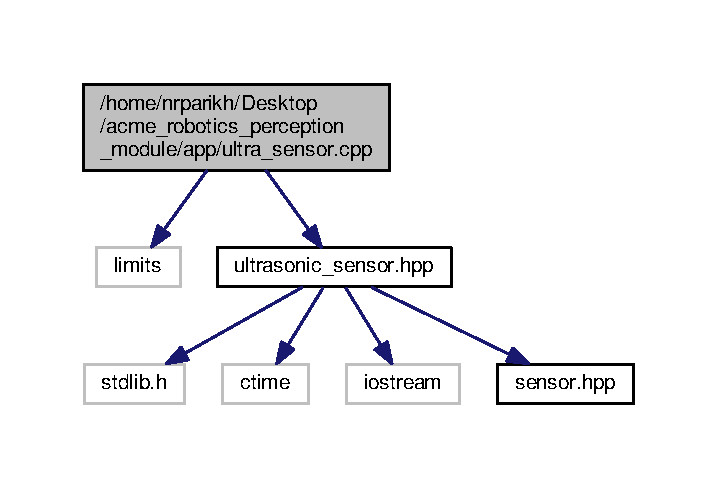
\includegraphics[width=344pt]{ultra__sensor_8cpp__incl}
\end{center}
\end{figure}

\hypertarget{camera_8hpp}{}\section{/home/nrparikh/\+Desktop/acme\+\_\+robotics\+\_\+perception\+\_\+module/include/camera.hpp File Reference}
\label{camera_8hpp}\index{/home/nrparikh/\+Desktop/acme\+\_\+robotics\+\_\+perception\+\_\+module/include/camera.\+hpp@{/home/nrparikh/\+Desktop/acme\+\_\+robotics\+\_\+perception\+\_\+module/include/camera.\+hpp}}


D\+E\+S\+C\+R\+I\+P\+T\+I\+ON Header file for the class \char`\"{}\+Camera\char`\"{}. This class is derived from the base class \char`\"{}\+Sensor\char`\"{}. The private members of the class include vid\+\_\+cap\+\_\+, is\+\_\+running\+\_\+, and output\+\_\+processed\+\_\+image\+\_\+. The get\+Output method returns the processed image while the process method processes the image suitable for finding the center of the contours.  


{\ttfamily \#include $<$opencv2/core.\+hpp$>$}\\*
{\ttfamily \#include $<$opencv2/highgui.\+hpp$>$}\\*
{\ttfamily \#include $<$opencv2/imgproc.\+hpp$>$}\\*
{\ttfamily \#include $<$opencv2/videoio.\+hpp$>$}\\*
{\ttfamily \#include $<$iostream$>$}\\*
{\ttfamily \#include $<$string$>$}\\*
{\ttfamily \#include \char`\"{}sensor.\+hpp\char`\"{}}\\*
Include dependency graph for camera.\+hpp\+:
\nopagebreak
\begin{figure}[H]
\begin{center}
\leavevmode
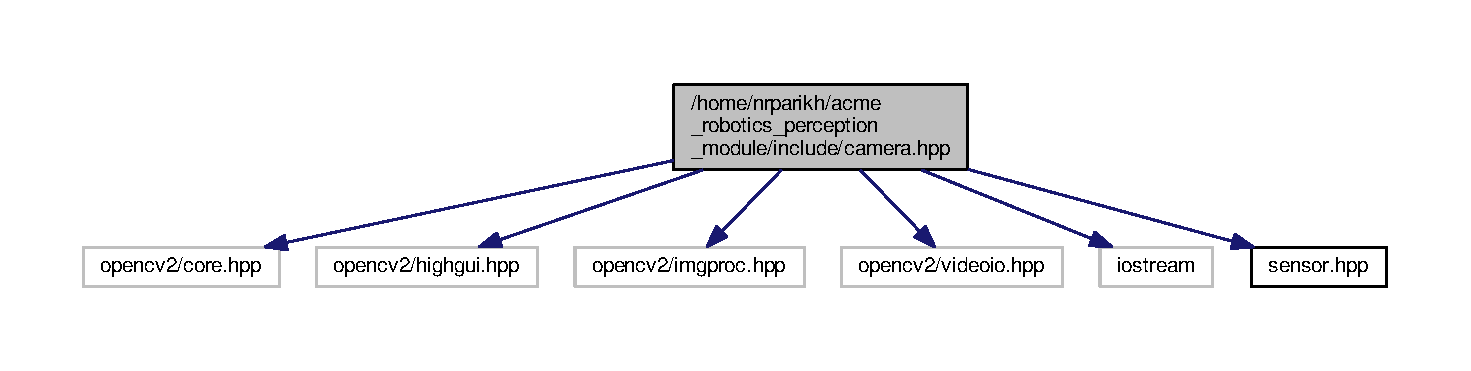
\includegraphics[width=350pt]{camera_8hpp__incl}
\end{center}
\end{figure}
This graph shows which files directly or indirectly include this file\+:
\nopagebreak
\begin{figure}[H]
\begin{center}
\leavevmode
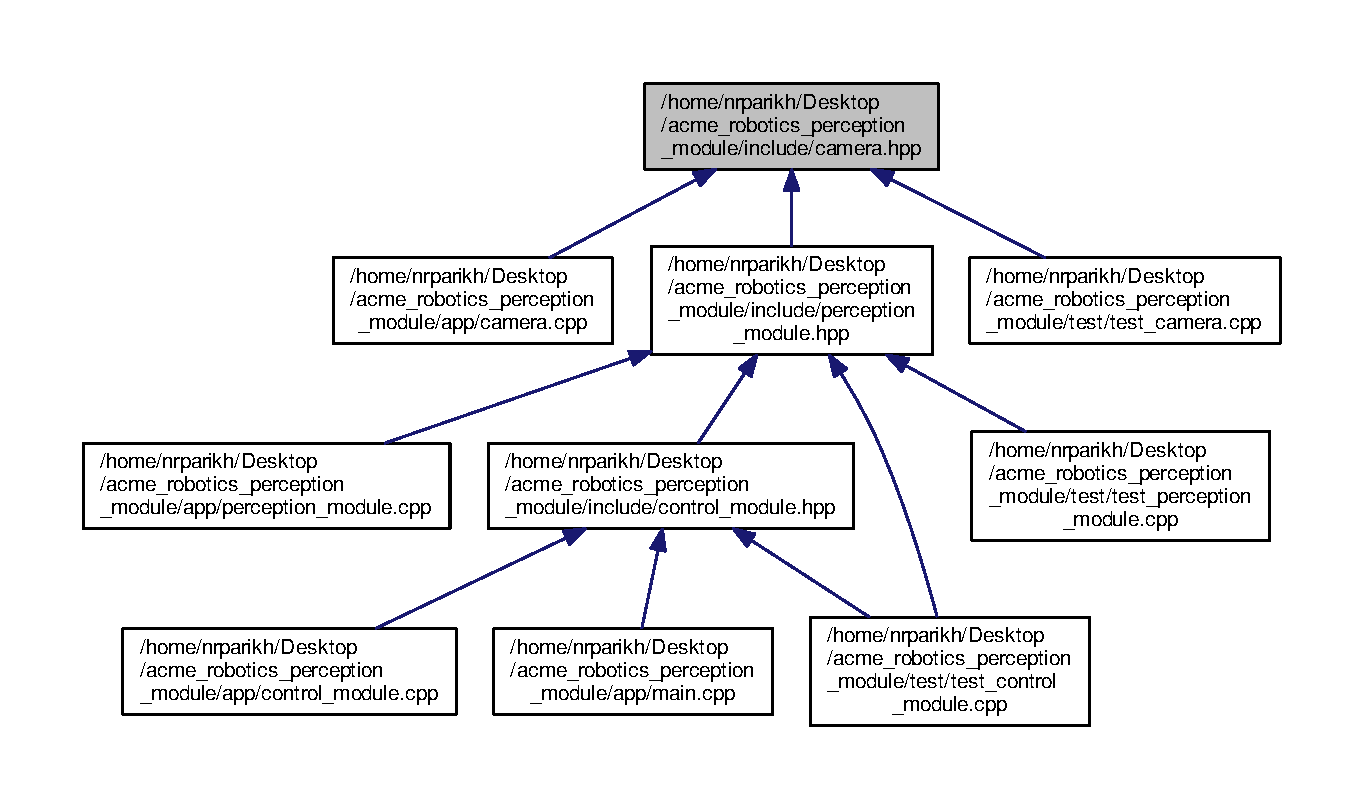
\includegraphics[width=350pt]{camera_8hpp__dep__incl}
\end{center}
\end{figure}
\subsection*{Classes}
\begin{DoxyCompactItemize}
\item 
class \hyperlink{class_camera}{Camera}
\begin{DoxyCompactList}\small\item\em Class for camera sensor. This class is derived from the base Class \hyperlink{class_sensor}{Sensor}. \end{DoxyCompactList}\end{DoxyCompactItemize}
\subsection*{Macros}
\begin{DoxyCompactItemize}
\item 
\#define \hyperlink{camera_8hpp_ac0543811059575e953053b2d1820d482}{D\+E\+B\+U\+G\+\_\+\+C\+A\+M\+E\+RA}
\end{DoxyCompactItemize}


\subsection{Detailed Description}
D\+E\+S\+C\+R\+I\+P\+T\+I\+ON Header file for the class \char`\"{}\+Camera\char`\"{}. This class is derived from the base class \char`\"{}\+Sensor\char`\"{}. The private members of the class include vid\+\_\+cap\+\_\+, is\+\_\+running\+\_\+, and output\+\_\+processed\+\_\+image\+\_\+. The get\+Output method returns the processed image while the process method processes the image suitable for finding the center of the contours. 

\begin{DoxyAuthor}{Author}
nrparikh 
\end{DoxyAuthor}
\begin{DoxyCopyright}{Copyright}
M\+IT license 
\end{DoxyCopyright}


\subsection{Macro Definition Documentation}
\index{camera.\+hpp@{camera.\+hpp}!D\+E\+B\+U\+G\+\_\+\+C\+A\+M\+E\+RA@{D\+E\+B\+U\+G\+\_\+\+C\+A\+M\+E\+RA}}
\index{D\+E\+B\+U\+G\+\_\+\+C\+A\+M\+E\+RA@{D\+E\+B\+U\+G\+\_\+\+C\+A\+M\+E\+RA}!camera.\+hpp@{camera.\+hpp}}
\subsubsection[{\texorpdfstring{D\+E\+B\+U\+G\+\_\+\+C\+A\+M\+E\+RA}{DEBUG_CAMERA}}]{\setlength{\rightskip}{0pt plus 5cm}\#define D\+E\+B\+U\+G\+\_\+\+C\+A\+M\+E\+RA}\hypertarget{camera_8hpp_ac0543811059575e953053b2d1820d482}{}\label{camera_8hpp_ac0543811059575e953053b2d1820d482}


Definition at line 27 of file camera.\+hpp.


\hypertarget{control__module_8hpp}{}\section{/home/nrparikh/\+Desktop/acme\+\_\+robotics\+\_\+perception\+\_\+module/include/control\+\_\+module.hpp File Reference}
\label{control__module_8hpp}\index{/home/nrparikh/\+Desktop/acme\+\_\+robotics\+\_\+perception\+\_\+module/include/control\+\_\+module.\+hpp@{/home/nrparikh/\+Desktop/acme\+\_\+robotics\+\_\+perception\+\_\+module/include/control\+\_\+module.\+hpp}}


D\+E\+S\+C\+R\+I\+P\+T\+I\+ON Header file for the class \char`\"{}\+Control\+Module\char`\"{}. This class is the control module which gets the readings from the Ultrasonic sensor as well as the center of the contour from the camera module. It processes this information and decides what action needs to be taken.  


{\ttfamily \#include $<$math.\+h$>$}\\*
{\ttfamily \#include $<$iostream$>$}\\*
{\ttfamily \#include $<$memory$>$}\\*
{\ttfamily \#include $<$string$>$}\\*
{\ttfamily \#include $<$utility$>$}\\*
{\ttfamily \#include $<$vector$>$}\\*
{\ttfamily \#include \char`\"{}perception\+\_\+module.\+hpp\char`\"{}}\\*
{\ttfamily \#include \char`\"{}ultrasonic\+\_\+sensor.\+hpp\char`\"{}}\\*
Include dependency graph for control\+\_\+module.\+hpp\+:
\nopagebreak
\begin{figure}[H]
\begin{center}
\leavevmode
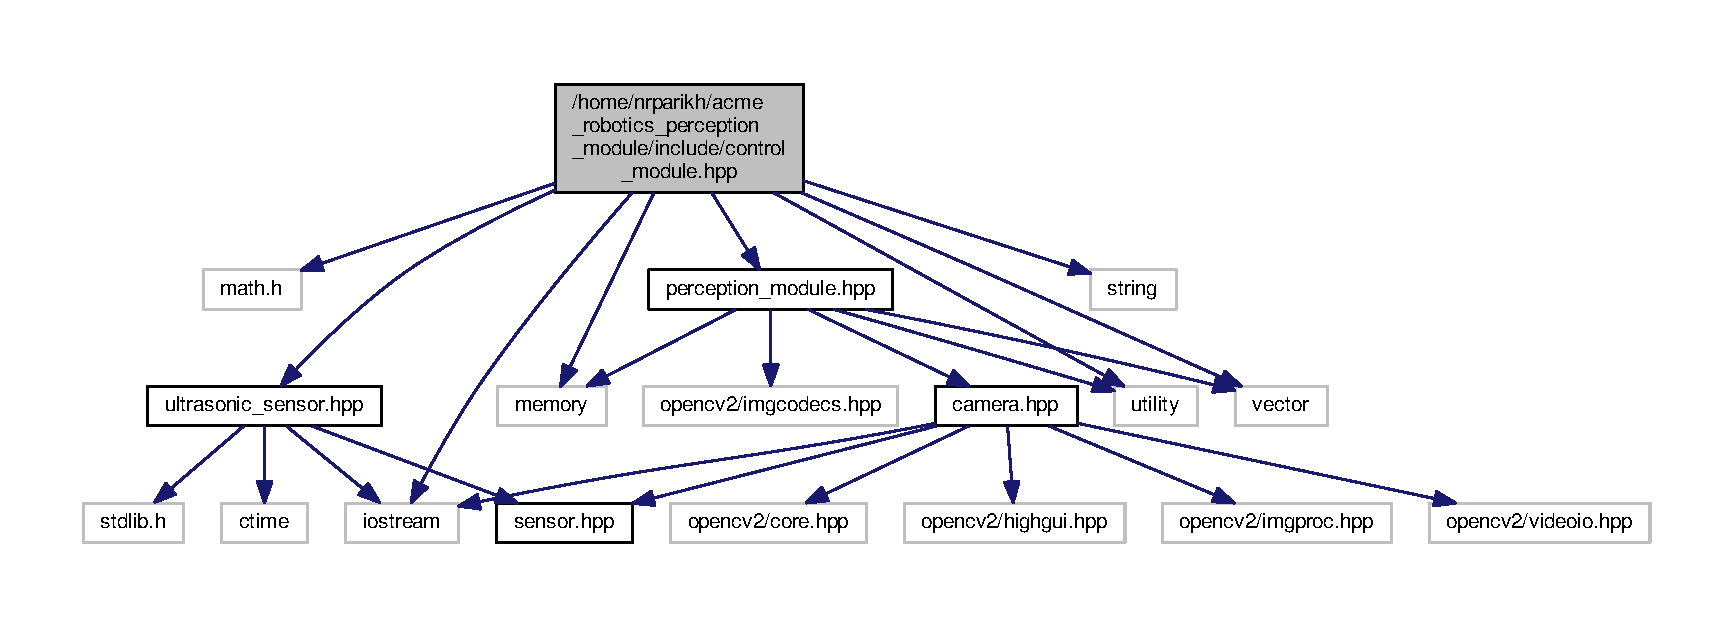
\includegraphics[width=350pt]{control__module_8hpp__incl}
\end{center}
\end{figure}
This graph shows which files directly or indirectly include this file\+:
\nopagebreak
\begin{figure}[H]
\begin{center}
\leavevmode
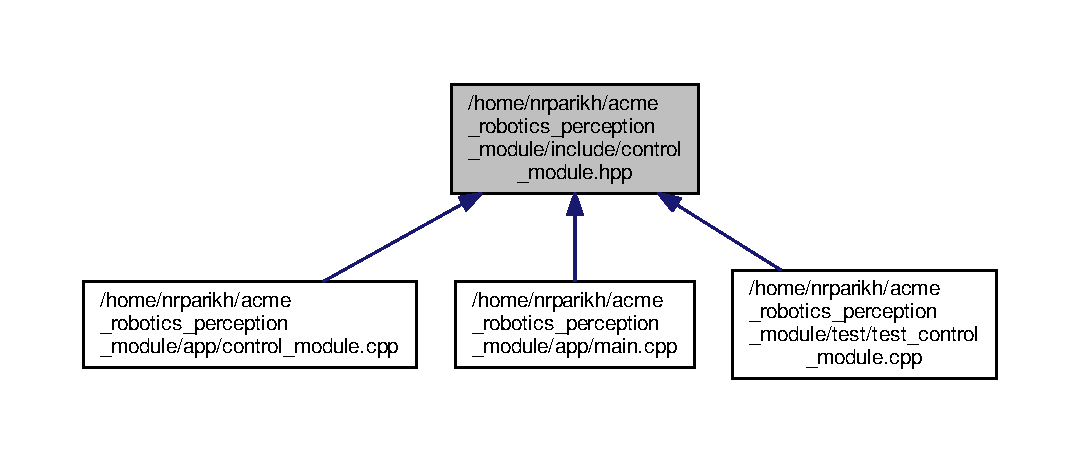
\includegraphics[width=350pt]{control__module_8hpp__dep__incl}
\end{center}
\end{figure}
\subsection*{Classes}
\begin{DoxyCompactItemize}
\item 
class \hyperlink{class_control_module}{Control\+Module}
\begin{DoxyCompactList}\small\item\em Class for control module. This class generates the actions based on the inputs from ultrasonic sensor and camera. \end{DoxyCompactList}\end{DoxyCompactItemize}


\subsection{Detailed Description}
D\+E\+S\+C\+R\+I\+P\+T\+I\+ON Header file for the class \char`\"{}\+Control\+Module\char`\"{}. This class is the control module which gets the readings from the Ultrasonic sensor as well as the center of the contour from the camera module. It processes this information and decides what action needs to be taken. 

\begin{DoxyAuthor}{Author}
nrparikh 
\end{DoxyAuthor}
\begin{DoxyCopyright}{Copyright}
M\+IT license 
\end{DoxyCopyright}

\hypertarget{perception__module_8hpp}{}\section{/home/nrparikh/acme\+\_\+robotics\+\_\+perception\+\_\+module/include/perception\+\_\+module.hpp File Reference}
\label{perception__module_8hpp}\index{/home/nrparikh/acme\+\_\+robotics\+\_\+perception\+\_\+module/include/perception\+\_\+module.\+hpp@{/home/nrparikh/acme\+\_\+robotics\+\_\+perception\+\_\+module/include/perception\+\_\+module.\+hpp}}


D\+E\+S\+C\+R\+I\+P\+T\+I\+ON Header file for the class \char`\"{}\+Perception\+Module\char`\"{}. This class gets the pre-\/processed image as an input and finds the contours in the image. It then finds the center of the contours which is the output of the class. This center is then passed on to the \char`\"{}\+Controller\char`\"{} module.  


{\ttfamily \#include $<$opencv2/imgcodecs.\+hpp$>$}\\*
{\ttfamily \#include $<$memory$>$}\\*
{\ttfamily \#include $<$utility$>$}\\*
{\ttfamily \#include $<$vector$>$}\\*
{\ttfamily \#include \char`\"{}camera.\+hpp\char`\"{}}\\*
Include dependency graph for perception\+\_\+module.\+hpp\+:
\nopagebreak
\begin{figure}[H]
\begin{center}
\leavevmode
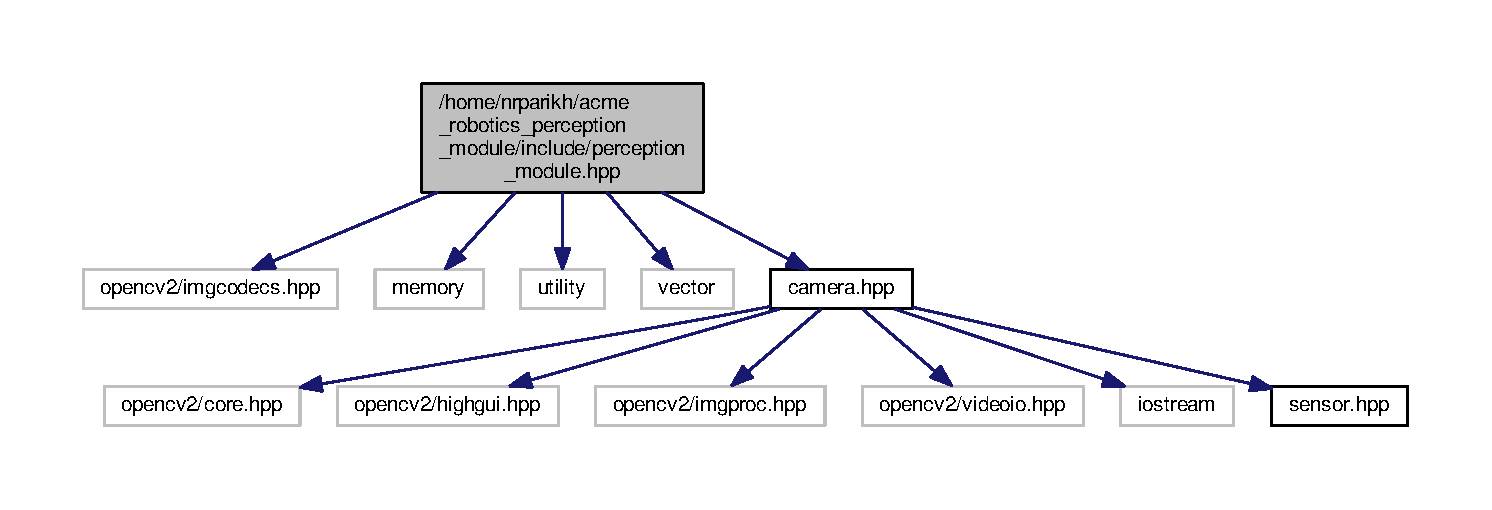
\includegraphics[width=350pt]{perception__module_8hpp__incl}
\end{center}
\end{figure}
This graph shows which files directly or indirectly include this file\+:
\nopagebreak
\begin{figure}[H]
\begin{center}
\leavevmode
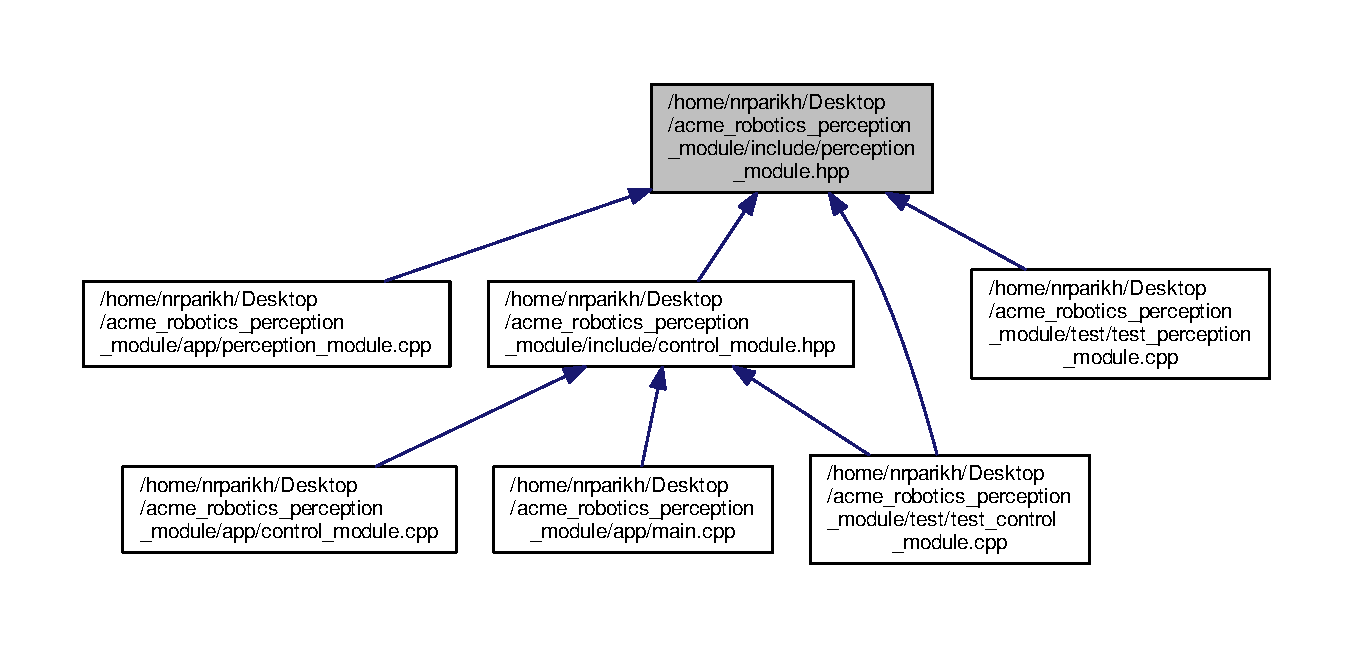
\includegraphics[width=350pt]{perception__module_8hpp__dep__incl}
\end{center}
\end{figure}
\subsection*{Classes}
\begin{DoxyCompactItemize}
\item 
class \hyperlink{class_perception_module}{Perception\+Module}
\begin{DoxyCompactList}\small\item\em Class for perception module. This class finds the contours and the center of the contours in the image provided as an input. \end{DoxyCompactList}\end{DoxyCompactItemize}


\subsection{Detailed Description}
D\+E\+S\+C\+R\+I\+P\+T\+I\+ON Header file for the class \char`\"{}\+Perception\+Module\char`\"{}. This class gets the pre-\/processed image as an input and finds the contours in the image. It then finds the center of the contours which is the output of the class. This center is then passed on to the \char`\"{}\+Controller\char`\"{} module. 

\begin{DoxyAuthor}{Author}
nrparikh 
\end{DoxyAuthor}
\begin{DoxyCopyright}{Copyright}
M\+IT license 
\end{DoxyCopyright}

\hypertarget{sensor_8hpp}{}\section{/home/nrparikh/acme\+\_\+robotics\+\_\+perception\+\_\+module/include/sensor.hpp File Reference}
\label{sensor_8hpp}\index{/home/nrparikh/acme\+\_\+robotics\+\_\+perception\+\_\+module/include/sensor.\+hpp@{/home/nrparikh/acme\+\_\+robotics\+\_\+perception\+\_\+module/include/sensor.\+hpp}}


D\+E\+S\+C\+R\+I\+P\+T\+I\+ON Header filer for the generic class \char`\"{}\+Sensor\char`\"{}. This is the base class which the required modules can derive from. The class has generic virtual methods get\+Output and process. The methods should be overloaded by the derived class.  


This graph shows which files directly or indirectly include this file\+:
\nopagebreak
\begin{figure}[H]
\begin{center}
\leavevmode
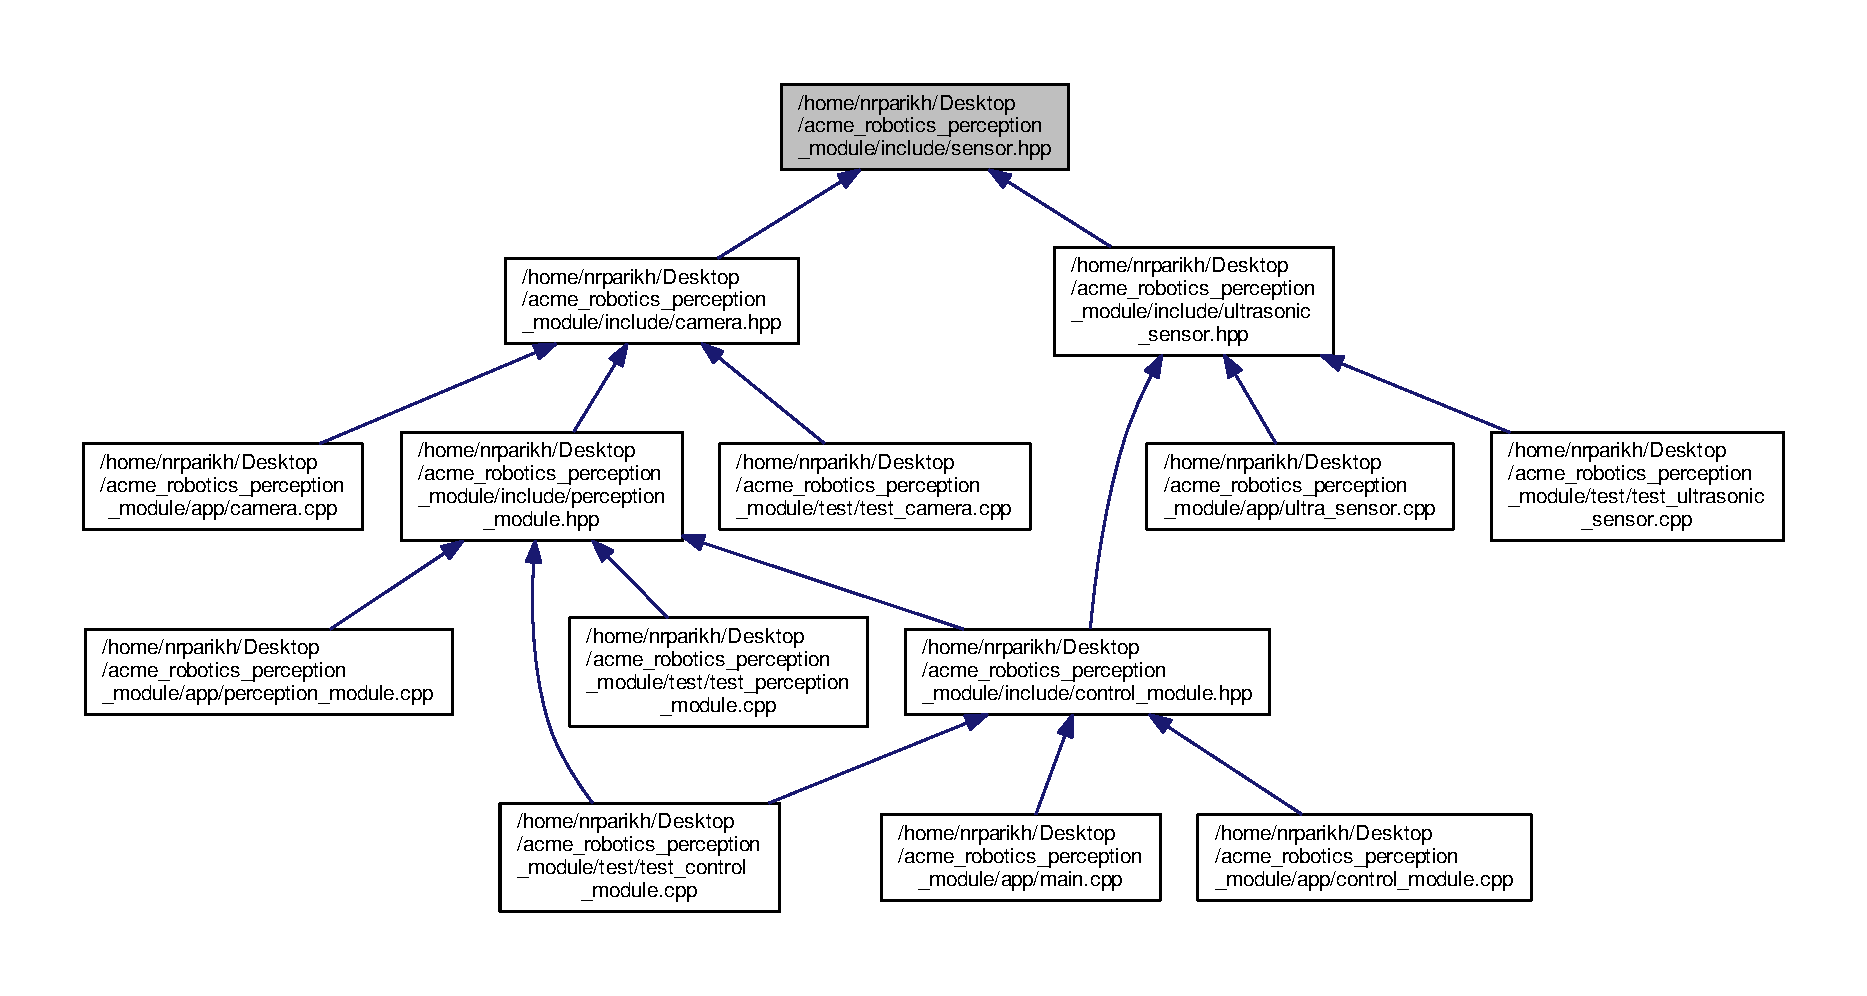
\includegraphics[width=350pt]{sensor_8hpp__dep__incl}
\end{center}
\end{figure}
\subsection*{Classes}
\begin{DoxyCompactItemize}
\item 
class \hyperlink{class_sensor}{Sensor$<$ T $>$}
\begin{DoxyCompactList}\small\item\em Class for generic sensor. Particular sensor in the system will inherit this base class. \end{DoxyCompactList}\end{DoxyCompactItemize}


\subsection{Detailed Description}
D\+E\+S\+C\+R\+I\+P\+T\+I\+ON Header filer for the generic class \char`\"{}\+Sensor\char`\"{}. This is the base class which the required modules can derive from. The class has generic virtual methods get\+Output and process. The methods should be overloaded by the derived class. 

\begin{DoxyAuthor}{Author}
nrparikh 
\end{DoxyAuthor}
\begin{DoxyCopyright}{Copyright}
M\+IT license 
\end{DoxyCopyright}

\hypertarget{ultrasonic__sensor_8hpp}{}\section{/home/nrparikh/\+Desktop/acme\+\_\+robotics\+\_\+perception\+\_\+module/include/ultrasonic\+\_\+sensor.hpp File Reference}
\label{ultrasonic__sensor_8hpp}\index{/home/nrparikh/\+Desktop/acme\+\_\+robotics\+\_\+perception\+\_\+module/include/ultrasonic\+\_\+sensor.\+hpp@{/home/nrparikh/\+Desktop/acme\+\_\+robotics\+\_\+perception\+\_\+module/include/ultrasonic\+\_\+sensor.\+hpp}}


D\+E\+S\+C\+R\+I\+P\+T\+I\+ON Header file for the class \char`\"{}\+Ultrasonic\+Sensor\char`\"{}. This class is derived from the base class \char`\"{}\+Sensor\char`\"{}. It has private members as max\+\_\+distance\+\_\+, is\+\_\+running\+\_\+ and output\+\_\+current\+\_\+distance\+\_\+. The get\+Output method returns the current distance reading while process method updates the current distance reading.  


{\ttfamily \#include $<$stdlib.\+h$>$}\\*
{\ttfamily \#include $<$ctime$>$}\\*
{\ttfamily \#include $<$iostream$>$}\\*
{\ttfamily \#include \char`\"{}sensor.\+hpp\char`\"{}}\\*
Include dependency graph for ultrasonic\+\_\+sensor.\+hpp\+:
\nopagebreak
\begin{figure}[H]
\begin{center}
\leavevmode
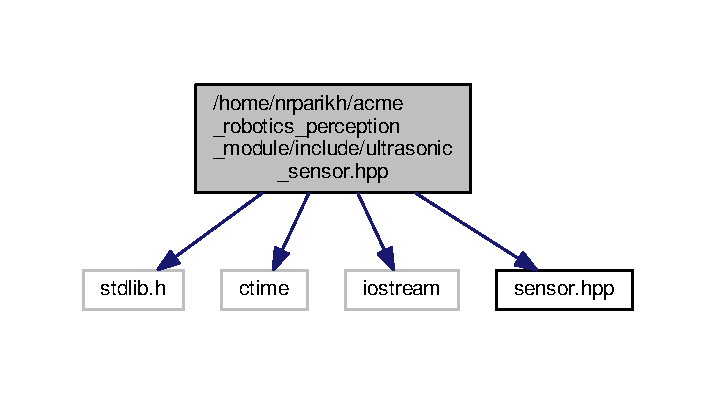
\includegraphics[width=344pt]{ultrasonic__sensor_8hpp__incl}
\end{center}
\end{figure}
This graph shows which files directly or indirectly include this file\+:
\nopagebreak
\begin{figure}[H]
\begin{center}
\leavevmode
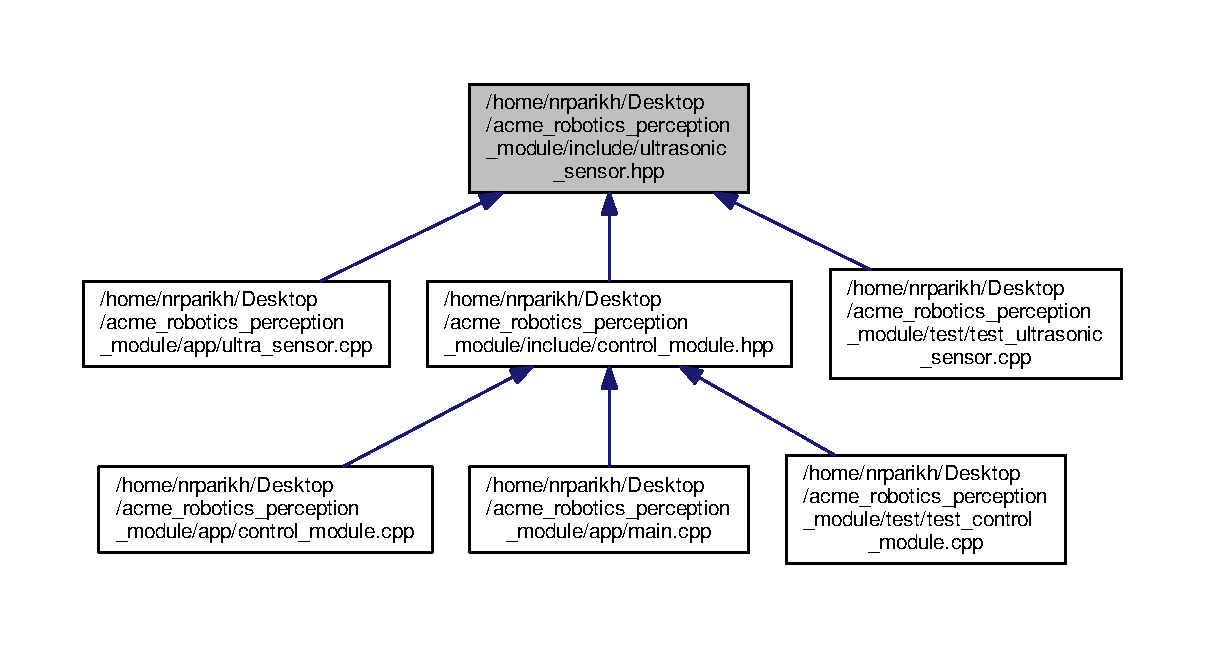
\includegraphics[width=350pt]{ultrasonic__sensor_8hpp__dep__incl}
\end{center}
\end{figure}
\subsection*{Classes}
\begin{DoxyCompactItemize}
\item 
class \hyperlink{class_ultrasonic_sensor}{Ultrasonic\+Sensor}
\end{DoxyCompactItemize}


\subsection{Detailed Description}
D\+E\+S\+C\+R\+I\+P\+T\+I\+ON Header file for the class \char`\"{}\+Ultrasonic\+Sensor\char`\"{}. This class is derived from the base class \char`\"{}\+Sensor\char`\"{}. It has private members as max\+\_\+distance\+\_\+, is\+\_\+running\+\_\+ and output\+\_\+current\+\_\+distance\+\_\+. The get\+Output method returns the current distance reading while process method updates the current distance reading. 

\begin{DoxyAuthor}{Author}
nrparikh 
\end{DoxyAuthor}
\begin{DoxyCopyright}{Copyright}
M\+IT license 
\end{DoxyCopyright}

\hypertarget{readme_8md}{}\section{/home/nrparikh/acme\+\_\+robotics\+\_\+perception\+\_\+module/readme.md File Reference}
\label{readme_8md}\index{/home/nrparikh/acme\+\_\+robotics\+\_\+perception\+\_\+module/readme.\+md@{/home/nrparikh/acme\+\_\+robotics\+\_\+perception\+\_\+module/readme.\+md}}

\hypertarget{test__camera_8cpp}{}\section{/home/nrparikh/\+Desktop/acme\+\_\+robotics\+\_\+perception\+\_\+module/test/test\+\_\+camera.cpp File Reference}
\label{test__camera_8cpp}\index{/home/nrparikh/\+Desktop/acme\+\_\+robotics\+\_\+perception\+\_\+module/test/test\+\_\+camera.\+cpp@{/home/nrparikh/\+Desktop/acme\+\_\+robotics\+\_\+perception\+\_\+module/test/test\+\_\+camera.\+cpp}}


D\+E\+S\+C\+R\+I\+P\+T\+I\+ON Testing file for the \hyperlink{class_camera}{Camera} class.  


{\ttfamily \#include $<$gtest/gtest.\+h$>$}\\*
{\ttfamily \#include $<$opencv2/core.\+hpp$>$}\\*
{\ttfamily \#include $<$opencv2/highgui.\+hpp$>$}\\*
{\ttfamily \#include $<$opencv2/imgproc.\+hpp$>$}\\*
{\ttfamily \#include \char`\"{}camera.\+hpp\char`\"{}}\\*
Include dependency graph for test\+\_\+camera.\+cpp\+:
\nopagebreak
\begin{figure}[H]
\begin{center}
\leavevmode
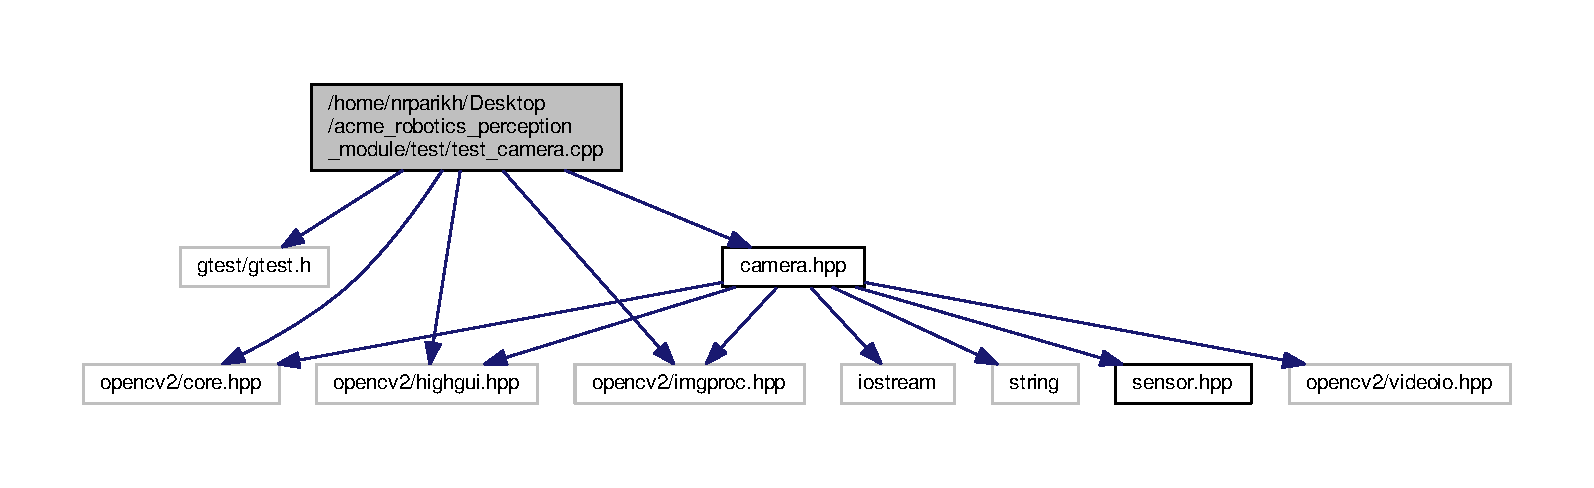
\includegraphics[width=350pt]{test__camera_8cpp__incl}
\end{center}
\end{figure}
\subsection*{Classes}
\begin{DoxyCompactItemize}
\item 
class \hyperlink{class_test_camera}{Test\+Camera}
\begin{DoxyCompactList}\small\item\em Class for the testing of \hyperlink{class_camera}{Camera} class. Creates a protected camera object which can be used for testing. \end{DoxyCompactList}\end{DoxyCompactItemize}
\subsection*{Functions}
\begin{DoxyCompactItemize}
\item 
\hyperlink{test__camera_8cpp_adb94cbb41f33e01b9c0e7d230cb8539a}{T\+E\+S\+T\+\_\+F} (\hyperlink{class_test_camera}{Test\+Camera}, dummy\+Test)
\begin{DoxyCompactList}\small\item\em Dummy test function to check the working of tests. \end{DoxyCompactList}\item 
\hyperlink{test__camera_8cpp_a567a0a23089144c979a566b333166ccc}{T\+E\+S\+T\+\_\+F} (\hyperlink{class_test_camera}{Test\+Camera}, is\+Alive)
\begin{DoxyCompactList}\small\item\em Test to check the working of camera module. \end{DoxyCompactList}\item 
\hyperlink{test__camera_8cpp_a2418eab8b2f10c97a03e62e253fae29a}{T\+E\+S\+T\+\_\+F} (\hyperlink{class_test_camera}{Test\+Camera}, default\+Video\+Setup)
\begin{DoxyCompactList}\small\item\em Test to check default video setup method. \end{DoxyCompactList}\end{DoxyCompactItemize}


\subsection{Detailed Description}
D\+E\+S\+C\+R\+I\+P\+T\+I\+ON Testing file for the \hyperlink{class_camera}{Camera} class. 

\begin{DoxyAuthor}{Author}
nrparikh 
\end{DoxyAuthor}
\begin{DoxyCopyright}{Copyright}
M\+IT license 
\end{DoxyCopyright}


\subsection{Function Documentation}
\index{test\+\_\+camera.\+cpp@{test\+\_\+camera.\+cpp}!T\+E\+S\+T\+\_\+F@{T\+E\+S\+T\+\_\+F}}
\index{T\+E\+S\+T\+\_\+F@{T\+E\+S\+T\+\_\+F}!test\+\_\+camera.\+cpp@{test\+\_\+camera.\+cpp}}
\subsubsection[{\texorpdfstring{T\+E\+S\+T\+\_\+\+F(\+Test\+Camera, dummy\+Test)}{TEST_F(TestCamera, dummyTest)}}]{\setlength{\rightskip}{0pt plus 5cm}T\+E\+S\+T\+\_\+F (
\begin{DoxyParamCaption}
\item[{{\bf Test\+Camera}}]{, }
\item[{dummy\+Test}]{}
\end{DoxyParamCaption}
)}\hypertarget{test__camera_8cpp_adb94cbb41f33e01b9c0e7d230cb8539a}{}\label{test__camera_8cpp_adb94cbb41f33e01b9c0e7d230cb8539a}


Dummy test function to check the working of tests. 



Definition at line 28 of file test\+\_\+camera.\+cpp.

\index{test\+\_\+camera.\+cpp@{test\+\_\+camera.\+cpp}!T\+E\+S\+T\+\_\+F@{T\+E\+S\+T\+\_\+F}}
\index{T\+E\+S\+T\+\_\+F@{T\+E\+S\+T\+\_\+F}!test\+\_\+camera.\+cpp@{test\+\_\+camera.\+cpp}}
\subsubsection[{\texorpdfstring{T\+E\+S\+T\+\_\+\+F(\+Test\+Camera, is\+Alive)}{TEST_F(TestCamera, isAlive)}}]{\setlength{\rightskip}{0pt plus 5cm}T\+E\+S\+T\+\_\+F (
\begin{DoxyParamCaption}
\item[{{\bf Test\+Camera}}]{, }
\item[{is\+Alive}]{}
\end{DoxyParamCaption}
)}\hypertarget{test__camera_8cpp_a567a0a23089144c979a566b333166ccc}{}\label{test__camera_8cpp_a567a0a23089144c979a566b333166ccc}


Test to check the working of camera module. 



Definition at line 34 of file test\+\_\+camera.\+cpp.

\index{test\+\_\+camera.\+cpp@{test\+\_\+camera.\+cpp}!T\+E\+S\+T\+\_\+F@{T\+E\+S\+T\+\_\+F}}
\index{T\+E\+S\+T\+\_\+F@{T\+E\+S\+T\+\_\+F}!test\+\_\+camera.\+cpp@{test\+\_\+camera.\+cpp}}
\subsubsection[{\texorpdfstring{T\+E\+S\+T\+\_\+\+F(\+Test\+Camera, default\+Video\+Setup)}{TEST_F(TestCamera, defaultVideoSetup)}}]{\setlength{\rightskip}{0pt plus 5cm}T\+E\+S\+T\+\_\+F (
\begin{DoxyParamCaption}
\item[{{\bf Test\+Camera}}]{, }
\item[{default\+Video\+Setup}]{}
\end{DoxyParamCaption}
)}\hypertarget{test__camera_8cpp_a2418eab8b2f10c97a03e62e253fae29a}{}\label{test__camera_8cpp_a2418eab8b2f10c97a03e62e253fae29a}


Test to check default video setup method. 



Definition at line 41 of file test\+\_\+camera.\+cpp.


\hypertarget{test__control__module_8cpp}{}\section{/home/nrparikh/\+Desktop/acme\+\_\+robotics\+\_\+perception\+\_\+module/test/test\+\_\+control\+\_\+module.cpp File Reference}
\label{test__control__module_8cpp}\index{/home/nrparikh/\+Desktop/acme\+\_\+robotics\+\_\+perception\+\_\+module/test/test\+\_\+control\+\_\+module.\+cpp@{/home/nrparikh/\+Desktop/acme\+\_\+robotics\+\_\+perception\+\_\+module/test/test\+\_\+control\+\_\+module.\+cpp}}


D\+E\+S\+C\+R\+I\+P\+T\+I\+ON Testing file for the \hyperlink{class_control_module}{Control\+Module} class.  


{\ttfamily \#include $<$gtest/gtest.\+h$>$}\\*
{\ttfamily \#include \char`\"{}control\+\_\+module.\+hpp\char`\"{}}\\*
{\ttfamily \#include \char`\"{}perception\+\_\+module.\+hpp\char`\"{}}\\*
Include dependency graph for test\+\_\+control\+\_\+module.\+cpp\+:
\nopagebreak
\begin{figure}[H]
\begin{center}
\leavevmode
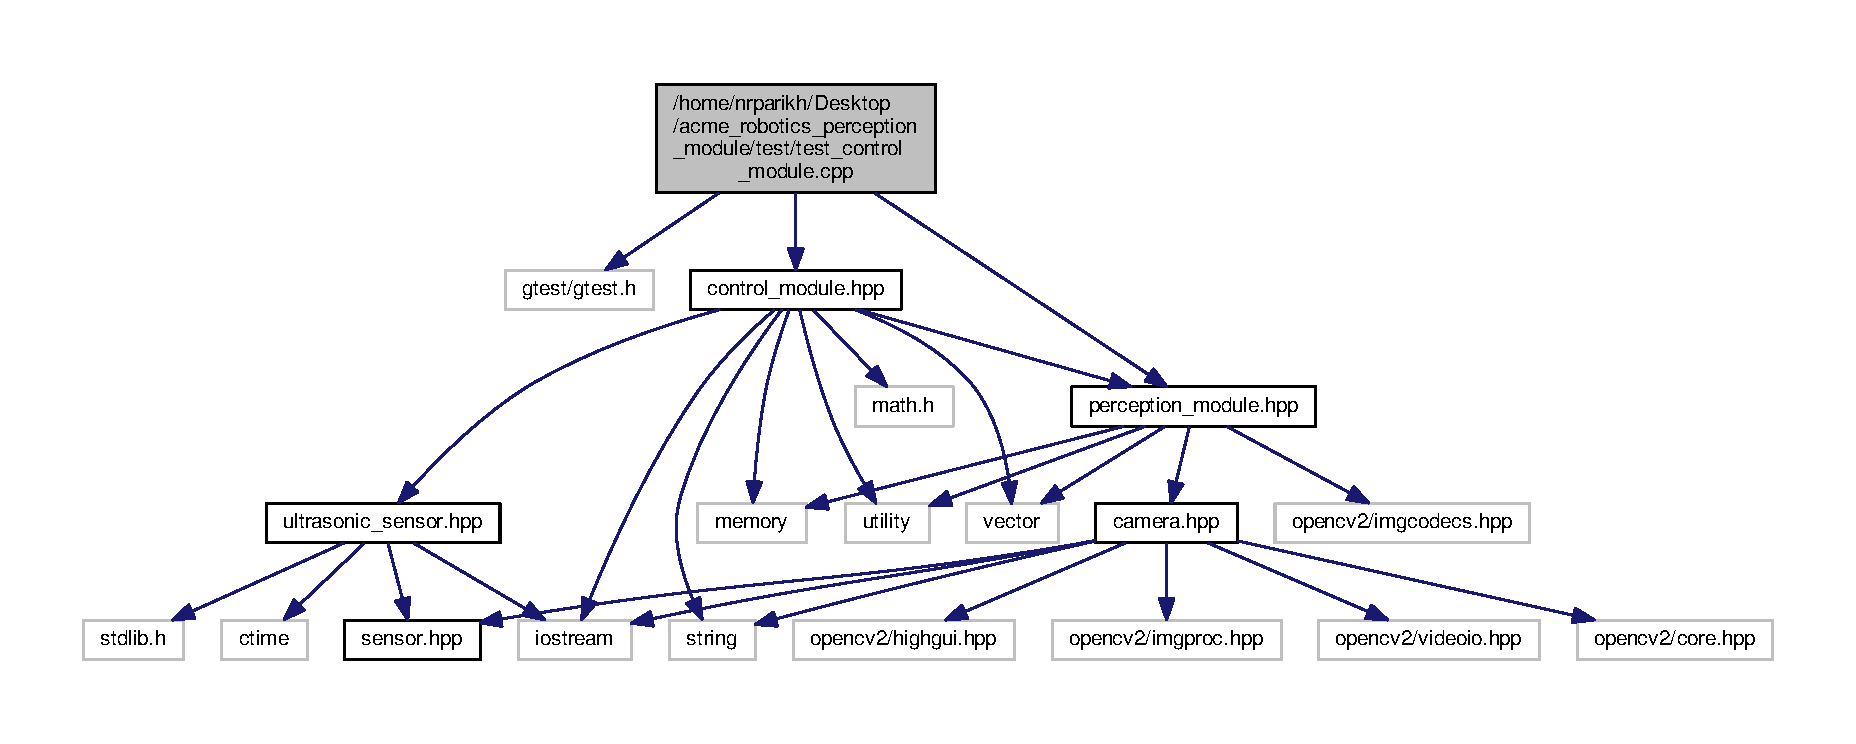
\includegraphics[width=350pt]{test__control__module_8cpp__incl}
\end{center}
\end{figure}
\subsection*{Classes}
\begin{DoxyCompactItemize}
\item 
class \hyperlink{class_test_control_module}{Test\+Control\+Module}
\begin{DoxyCompactList}\small\item\em Class for testing the \hyperlink{class_control_module}{Control\+Module} of the code. Create instances of perception and control modules which can be used later for testing. \end{DoxyCompactList}\end{DoxyCompactItemize}
\subsection*{Functions}
\begin{DoxyCompactItemize}
\item 
\hyperlink{test__control__module_8cpp_a90c0a3036c0322ba5fdb2dda29cfbc58}{T\+E\+S\+T\+\_\+F} (\hyperlink{class_test_control_module}{Test\+Control\+Module}, dummy\+Test)
\begin{DoxyCompactList}\small\item\em Dummy test to check the working of tests. \end{DoxyCompactList}\item 
\hyperlink{test__control__module_8cpp_a5c42f22ac2577a04542d06b795adedf1}{T\+E\+S\+T\+\_\+F} (\hyperlink{class_test_control_module}{Test\+Control\+Module}, is\+Alive)
\begin{DoxyCompactList}\small\item\em Test to check the working of control module. \end{DoxyCompactList}\item 
\hyperlink{test__control__module_8cpp_a084acacd2b5842670813a963cf1ea145}{T\+E\+S\+T\+\_\+F} (\hyperlink{class_test_control_module}{Test\+Control\+Module}, diagnostic\+Test)
\begin{DoxyCompactList}\small\item\em Test to run diagnostic tests for all modules. \end{DoxyCompactList}\item 
\hyperlink{test__control__module_8cpp_afca0d64766d83bc2def8445c006c47a8}{T\+E\+S\+T\+\_\+F} (\hyperlink{class_test_control_module}{Test\+Control\+Module}, process\+Working1)
\begin{DoxyCompactList}\small\item\em Test to check the working of the control module. \end{DoxyCompactList}\item 
\hyperlink{test__control__module_8cpp_abc58ab20df51258602c36a94f3432992}{T\+E\+S\+T\+\_\+F} (\hyperlink{class_test_control_module}{Test\+Control\+Module}, process\+Working2)
\item 
\hyperlink{test__control__module_8cpp_a5721355034d426df9413eed42ff9ccb7}{T\+E\+S\+T\+\_\+F} (\hyperlink{class_test_control_module}{Test\+Control\+Module}, process\+Working3)
\item 
\hyperlink{test__control__module_8cpp_aae4387a9eb7c8cea6d2228b653092f3c}{T\+E\+S\+T\+\_\+F} (\hyperlink{class_test_control_module}{Test\+Control\+Module}, process\+Working4)
\end{DoxyCompactItemize}


\subsection{Detailed Description}
D\+E\+S\+C\+R\+I\+P\+T\+I\+ON Testing file for the \hyperlink{class_control_module}{Control\+Module} class. 

\begin{DoxyAuthor}{Author}
nrparikh 
\end{DoxyAuthor}
\begin{DoxyCopyright}{Copyright}
M\+IT license 
\end{DoxyCopyright}


\subsection{Function Documentation}
\index{test\+\_\+control\+\_\+module.\+cpp@{test\+\_\+control\+\_\+module.\+cpp}!T\+E\+S\+T\+\_\+F@{T\+E\+S\+T\+\_\+F}}
\index{T\+E\+S\+T\+\_\+F@{T\+E\+S\+T\+\_\+F}!test\+\_\+control\+\_\+module.\+cpp@{test\+\_\+control\+\_\+module.\+cpp}}
\subsubsection[{\texorpdfstring{T\+E\+S\+T\+\_\+\+F(\+Test\+Control\+Module, dummy\+Test)}{TEST_F(TestControlModule, dummyTest)}}]{\setlength{\rightskip}{0pt plus 5cm}T\+E\+S\+T\+\_\+F (
\begin{DoxyParamCaption}
\item[{{\bf Test\+Control\+Module}}]{, }
\item[{dummy\+Test}]{}
\end{DoxyParamCaption}
)}\hypertarget{test__control__module_8cpp_a90c0a3036c0322ba5fdb2dda29cfbc58}{}\label{test__control__module_8cpp_a90c0a3036c0322ba5fdb2dda29cfbc58}


Dummy test to check the working of tests. 



Definition at line 26 of file test\+\_\+control\+\_\+module.\+cpp.

\index{test\+\_\+control\+\_\+module.\+cpp@{test\+\_\+control\+\_\+module.\+cpp}!T\+E\+S\+T\+\_\+F@{T\+E\+S\+T\+\_\+F}}
\index{T\+E\+S\+T\+\_\+F@{T\+E\+S\+T\+\_\+F}!test\+\_\+control\+\_\+module.\+cpp@{test\+\_\+control\+\_\+module.\+cpp}}
\subsubsection[{\texorpdfstring{T\+E\+S\+T\+\_\+\+F(\+Test\+Control\+Module, is\+Alive)}{TEST_F(TestControlModule, isAlive)}}]{\setlength{\rightskip}{0pt plus 5cm}T\+E\+S\+T\+\_\+F (
\begin{DoxyParamCaption}
\item[{{\bf Test\+Control\+Module}}]{, }
\item[{is\+Alive}]{}
\end{DoxyParamCaption}
)}\hypertarget{test__control__module_8cpp_a5c42f22ac2577a04542d06b795adedf1}{}\label{test__control__module_8cpp_a5c42f22ac2577a04542d06b795adedf1}


Test to check the working of control module. 



Definition at line 32 of file test\+\_\+control\+\_\+module.\+cpp.

\index{test\+\_\+control\+\_\+module.\+cpp@{test\+\_\+control\+\_\+module.\+cpp}!T\+E\+S\+T\+\_\+F@{T\+E\+S\+T\+\_\+F}}
\index{T\+E\+S\+T\+\_\+F@{T\+E\+S\+T\+\_\+F}!test\+\_\+control\+\_\+module.\+cpp@{test\+\_\+control\+\_\+module.\+cpp}}
\subsubsection[{\texorpdfstring{T\+E\+S\+T\+\_\+\+F(\+Test\+Control\+Module, diagnostic\+Test)}{TEST_F(TestControlModule, diagnosticTest)}}]{\setlength{\rightskip}{0pt plus 5cm}T\+E\+S\+T\+\_\+F (
\begin{DoxyParamCaption}
\item[{{\bf Test\+Control\+Module}}]{, }
\item[{diagnostic\+Test}]{}
\end{DoxyParamCaption}
)}\hypertarget{test__control__module_8cpp_a084acacd2b5842670813a963cf1ea145}{}\label{test__control__module_8cpp_a084acacd2b5842670813a963cf1ea145}


Test to run diagnostic tests for all modules. 



Definition at line 39 of file test\+\_\+control\+\_\+module.\+cpp.

\index{test\+\_\+control\+\_\+module.\+cpp@{test\+\_\+control\+\_\+module.\+cpp}!T\+E\+S\+T\+\_\+F@{T\+E\+S\+T\+\_\+F}}
\index{T\+E\+S\+T\+\_\+F@{T\+E\+S\+T\+\_\+F}!test\+\_\+control\+\_\+module.\+cpp@{test\+\_\+control\+\_\+module.\+cpp}}
\subsubsection[{\texorpdfstring{T\+E\+S\+T\+\_\+\+F(\+Test\+Control\+Module, process\+Working1)}{TEST_F(TestControlModule, processWorking1)}}]{\setlength{\rightskip}{0pt plus 5cm}T\+E\+S\+T\+\_\+F (
\begin{DoxyParamCaption}
\item[{{\bf Test\+Control\+Module}}]{, }
\item[{process\+Working1}]{}
\end{DoxyParamCaption}
)}\hypertarget{test__control__module_8cpp_afca0d64766d83bc2def8445c006c47a8}{}\label{test__control__module_8cpp_afca0d64766d83bc2def8445c006c47a8}


Test to check the working of the control module. 



Definition at line 46 of file test\+\_\+control\+\_\+module.\+cpp.

\index{test\+\_\+control\+\_\+module.\+cpp@{test\+\_\+control\+\_\+module.\+cpp}!T\+E\+S\+T\+\_\+F@{T\+E\+S\+T\+\_\+F}}
\index{T\+E\+S\+T\+\_\+F@{T\+E\+S\+T\+\_\+F}!test\+\_\+control\+\_\+module.\+cpp@{test\+\_\+control\+\_\+module.\+cpp}}
\subsubsection[{\texorpdfstring{T\+E\+S\+T\+\_\+\+F(\+Test\+Control\+Module, process\+Working2)}{TEST_F(TestControlModule, processWorking2)}}]{\setlength{\rightskip}{0pt plus 5cm}T\+E\+S\+T\+\_\+F (
\begin{DoxyParamCaption}
\item[{{\bf Test\+Control\+Module}}]{, }
\item[{process\+Working2}]{}
\end{DoxyParamCaption}
)}\hypertarget{test__control__module_8cpp_abc58ab20df51258602c36a94f3432992}{}\label{test__control__module_8cpp_abc58ab20df51258602c36a94f3432992}


Definition at line 57 of file test\+\_\+control\+\_\+module.\+cpp.

\index{test\+\_\+control\+\_\+module.\+cpp@{test\+\_\+control\+\_\+module.\+cpp}!T\+E\+S\+T\+\_\+F@{T\+E\+S\+T\+\_\+F}}
\index{T\+E\+S\+T\+\_\+F@{T\+E\+S\+T\+\_\+F}!test\+\_\+control\+\_\+module.\+cpp@{test\+\_\+control\+\_\+module.\+cpp}}
\subsubsection[{\texorpdfstring{T\+E\+S\+T\+\_\+\+F(\+Test\+Control\+Module, process\+Working3)}{TEST_F(TestControlModule, processWorking3)}}]{\setlength{\rightskip}{0pt plus 5cm}T\+E\+S\+T\+\_\+F (
\begin{DoxyParamCaption}
\item[{{\bf Test\+Control\+Module}}]{, }
\item[{process\+Working3}]{}
\end{DoxyParamCaption}
)}\hypertarget{test__control__module_8cpp_a5721355034d426df9413eed42ff9ccb7}{}\label{test__control__module_8cpp_a5721355034d426df9413eed42ff9ccb7}


Definition at line 68 of file test\+\_\+control\+\_\+module.\+cpp.

\index{test\+\_\+control\+\_\+module.\+cpp@{test\+\_\+control\+\_\+module.\+cpp}!T\+E\+S\+T\+\_\+F@{T\+E\+S\+T\+\_\+F}}
\index{T\+E\+S\+T\+\_\+F@{T\+E\+S\+T\+\_\+F}!test\+\_\+control\+\_\+module.\+cpp@{test\+\_\+control\+\_\+module.\+cpp}}
\subsubsection[{\texorpdfstring{T\+E\+S\+T\+\_\+\+F(\+Test\+Control\+Module, process\+Working4)}{TEST_F(TestControlModule, processWorking4)}}]{\setlength{\rightskip}{0pt plus 5cm}T\+E\+S\+T\+\_\+F (
\begin{DoxyParamCaption}
\item[{{\bf Test\+Control\+Module}}]{, }
\item[{process\+Working4}]{}
\end{DoxyParamCaption}
)}\hypertarget{test__control__module_8cpp_aae4387a9eb7c8cea6d2228b653092f3c}{}\label{test__control__module_8cpp_aae4387a9eb7c8cea6d2228b653092f3c}


Definition at line 79 of file test\+\_\+control\+\_\+module.\+cpp.


\hypertarget{test__perception__module_8cpp}{}\section{/home/nrparikh/\+Desktop/acme\+\_\+robotics\+\_\+perception\+\_\+module/test/test\+\_\+perception\+\_\+module.cpp File Reference}
\label{test__perception__module_8cpp}\index{/home/nrparikh/\+Desktop/acme\+\_\+robotics\+\_\+perception\+\_\+module/test/test\+\_\+perception\+\_\+module.\+cpp@{/home/nrparikh/\+Desktop/acme\+\_\+robotics\+\_\+perception\+\_\+module/test/test\+\_\+perception\+\_\+module.\+cpp}}


D\+E\+S\+C\+R\+I\+P\+T\+I\+ON Testing file for the \hyperlink{class_perception_module}{Perception\+Module} class.  


{\ttfamily \#include $<$gtest/gtest.\+h$>$}\\*
{\ttfamily \#include \char`\"{}perception\+\_\+module.\+hpp\char`\"{}}\\*
Include dependency graph for test\+\_\+perception\+\_\+module.\+cpp\+:
\nopagebreak
\begin{figure}[H]
\begin{center}
\leavevmode
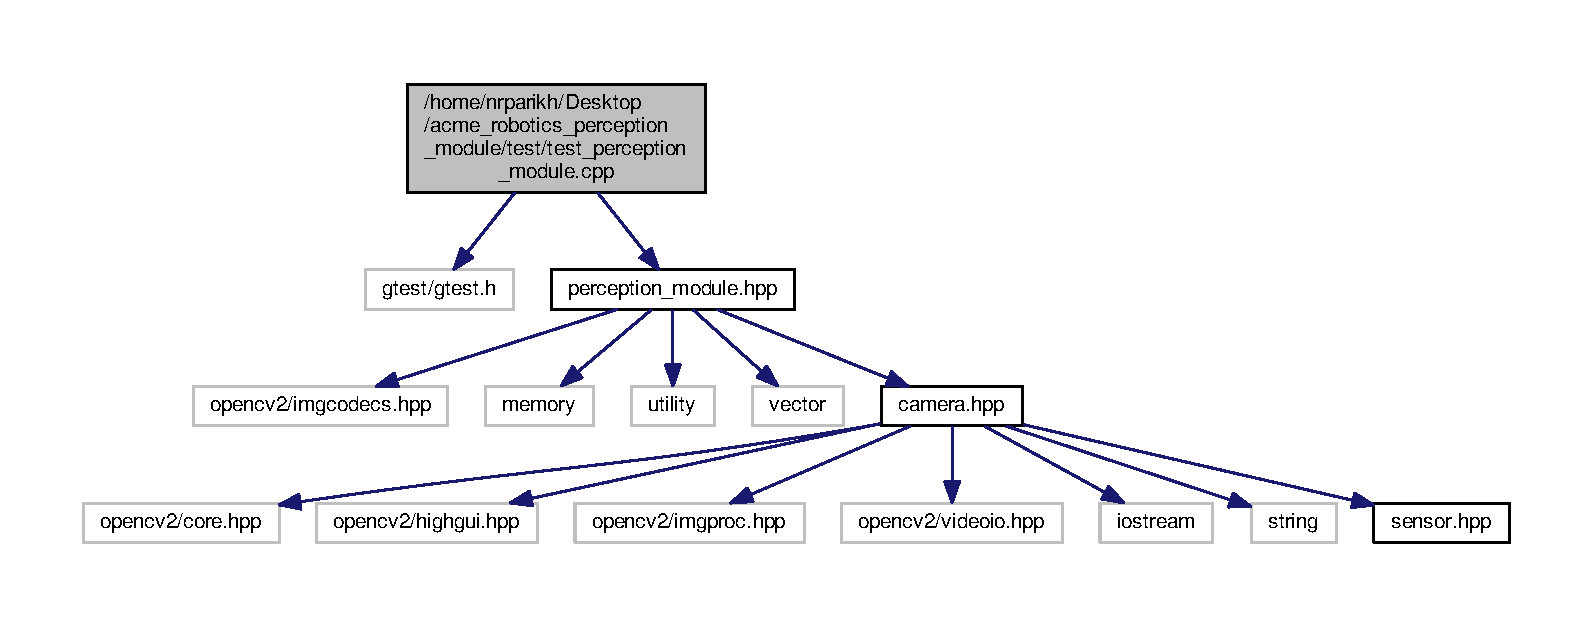
\includegraphics[width=350pt]{test__perception__module_8cpp__incl}
\end{center}
\end{figure}
\subsection*{Classes}
\begin{DoxyCompactItemize}
\item 
class \hyperlink{class_test_perception_module}{Test\+Perception\+Module}
\begin{DoxyCompactList}\small\item\em Class to test the working of \hyperlink{class_perception_module}{Perception\+Module}. Create an instance of perception module which can be used for testing. \end{DoxyCompactList}\end{DoxyCompactItemize}
\subsection*{Functions}
\begin{DoxyCompactItemize}
\item 
\hyperlink{test__perception__module_8cpp_a52e268e8b92e7a951727ce97813fda1f}{T\+E\+S\+T\+\_\+F} (\hyperlink{class_test_perception_module}{Test\+Perception\+Module}, dummy\+Test)
\begin{DoxyCompactList}\small\item\em Dummy test for testing the working of tests. \end{DoxyCompactList}\item 
\hyperlink{test__perception__module_8cpp_adfc407ed2e64006f06195e0b76bf958e}{T\+E\+S\+T\+\_\+F} (\hyperlink{class_test_perception_module}{Test\+Perception\+Module}, is\+Alive)
\begin{DoxyCompactList}\small\item\em Test ot check the working of perception module. \end{DoxyCompactList}\end{DoxyCompactItemize}


\subsection{Detailed Description}
D\+E\+S\+C\+R\+I\+P\+T\+I\+ON Testing file for the \hyperlink{class_perception_module}{Perception\+Module} class. 

\begin{DoxyAuthor}{Author}
nrparikh 
\end{DoxyAuthor}
\begin{DoxyCopyright}{Copyright}
M\+IT license 
\end{DoxyCopyright}


\subsection{Function Documentation}
\index{test\+\_\+perception\+\_\+module.\+cpp@{test\+\_\+perception\+\_\+module.\+cpp}!T\+E\+S\+T\+\_\+F@{T\+E\+S\+T\+\_\+F}}
\index{T\+E\+S\+T\+\_\+F@{T\+E\+S\+T\+\_\+F}!test\+\_\+perception\+\_\+module.\+cpp@{test\+\_\+perception\+\_\+module.\+cpp}}
\subsubsection[{\texorpdfstring{T\+E\+S\+T\+\_\+\+F(\+Test\+Perception\+Module, dummy\+Test)}{TEST_F(TestPerceptionModule, dummyTest)}}]{\setlength{\rightskip}{0pt plus 5cm}T\+E\+S\+T\+\_\+F (
\begin{DoxyParamCaption}
\item[{{\bf Test\+Perception\+Module}}]{, }
\item[{dummy\+Test}]{}
\end{DoxyParamCaption}
)}\hypertarget{test__perception__module_8cpp_a52e268e8b92e7a951727ce97813fda1f}{}\label{test__perception__module_8cpp_a52e268e8b92e7a951727ce97813fda1f}


Dummy test for testing the working of tests. 



Definition at line 25 of file test\+\_\+perception\+\_\+module.\+cpp.

\index{test\+\_\+perception\+\_\+module.\+cpp@{test\+\_\+perception\+\_\+module.\+cpp}!T\+E\+S\+T\+\_\+F@{T\+E\+S\+T\+\_\+F}}
\index{T\+E\+S\+T\+\_\+F@{T\+E\+S\+T\+\_\+F}!test\+\_\+perception\+\_\+module.\+cpp@{test\+\_\+perception\+\_\+module.\+cpp}}
\subsubsection[{\texorpdfstring{T\+E\+S\+T\+\_\+\+F(\+Test\+Perception\+Module, is\+Alive)}{TEST_F(TestPerceptionModule, isAlive)}}]{\setlength{\rightskip}{0pt plus 5cm}T\+E\+S\+T\+\_\+F (
\begin{DoxyParamCaption}
\item[{{\bf Test\+Perception\+Module}}]{, }
\item[{is\+Alive}]{}
\end{DoxyParamCaption}
)}\hypertarget{test__perception__module_8cpp_adfc407ed2e64006f06195e0b76bf958e}{}\label{test__perception__module_8cpp_adfc407ed2e64006f06195e0b76bf958e}


Test ot check the working of perception module. 



Definition at line 32 of file test\+\_\+perception\+\_\+module.\+cpp.


\hypertarget{test__ultrasonic__sensor_8cpp}{}\section{/home/nrparikh/\+Desktop/acme\+\_\+robotics\+\_\+perception\+\_\+module/test/test\+\_\+ultrasonic\+\_\+sensor.cpp File Reference}
\label{test__ultrasonic__sensor_8cpp}\index{/home/nrparikh/\+Desktop/acme\+\_\+robotics\+\_\+perception\+\_\+module/test/test\+\_\+ultrasonic\+\_\+sensor.\+cpp@{/home/nrparikh/\+Desktop/acme\+\_\+robotics\+\_\+perception\+\_\+module/test/test\+\_\+ultrasonic\+\_\+sensor.\+cpp}}


D\+E\+S\+C\+R\+I\+P\+T\+I\+ON Testing file for the \hyperlink{class_ultrasonic_sensor}{Ultrasonic\+Sensor}.  


{\ttfamily \#include $<$gtest/gtest.\+h$>$}\\*
{\ttfamily \#include $<$stdlib.\+h$>$}\\*
{\ttfamily \#include $<$ctime$>$}\\*
{\ttfamily \#include $<$iostream$>$}\\*
{\ttfamily \#include \char`\"{}ultrasonic\+\_\+sensor.\+hpp\char`\"{}}\\*
Include dependency graph for test\+\_\+ultrasonic\+\_\+sensor.\+cpp\+:
\nopagebreak
\begin{figure}[H]
\begin{center}
\leavevmode
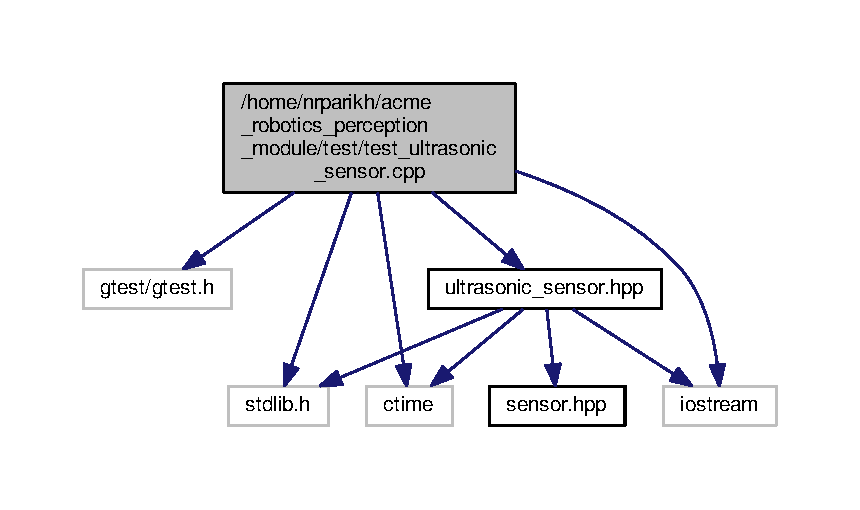
\includegraphics[width=350pt]{test__ultrasonic__sensor_8cpp__incl}
\end{center}
\end{figure}
\subsection*{Classes}
\begin{DoxyCompactItemize}
\item 
class \hyperlink{class_test_ultrasonic_sensor}{Test\+Ultrasonic\+Sensor}
\begin{DoxyCompactList}\small\item\em Class to test the working of Ultrasonic sensor. Create an instance of ultrasonic sensor which can be used for testing. \end{DoxyCompactList}\end{DoxyCompactItemize}
\subsection*{Functions}
\begin{DoxyCompactItemize}
\item 
\hyperlink{test__ultrasonic__sensor_8cpp_a8ea3edb56b5e241c4f4fd452ae424928}{T\+E\+S\+T\+\_\+F} (\hyperlink{class_test_ultrasonic_sensor}{Test\+Ultrasonic\+Sensor}, dummy\+Test)
\begin{DoxyCompactList}\small\item\em Dummy test to check the working of tests. \end{DoxyCompactList}\item 
\hyperlink{test__ultrasonic__sensor_8cpp_a5aee3e994357bd4252e35d0d9d52b792}{T\+E\+S\+T\+\_\+F} (\hyperlink{class_test_ultrasonic_sensor}{Test\+Ultrasonic\+Sensor}, is\+Alive)
\begin{DoxyCompactList}\small\item\em Test to check the working of ultrasonic sensor. \end{DoxyCompactList}\item 
\hyperlink{test__ultrasonic__sensor_8cpp_a905af2a4643ccc581de144bd39c0fe19}{T\+E\+S\+T\+\_\+F} (\hyperlink{class_test_ultrasonic_sensor}{Test\+Ultrasonic\+Sensor}, set\+Max\+Distance)
\begin{DoxyCompactList}\small\item\em Test to check the method of setting maximum distance. \end{DoxyCompactList}\item 
\hyperlink{test__ultrasonic__sensor_8cpp_a52d10f574675b80fa658fa710c00531d}{T\+E\+S\+T\+\_\+F} (\hyperlink{class_test_ultrasonic_sensor}{Test\+Ultrasonic\+Sensor}, sensor\+Reading)
\begin{DoxyCompactList}\small\item\em Test to check the reading of ultrasonic sensor. \end{DoxyCompactList}\end{DoxyCompactItemize}


\subsection{Detailed Description}
D\+E\+S\+C\+R\+I\+P\+T\+I\+ON Testing file for the \hyperlink{class_ultrasonic_sensor}{Ultrasonic\+Sensor}. 

\begin{DoxyAuthor}{Author}
nrparikh 
\end{DoxyAuthor}
\begin{DoxyCopyright}{Copyright}
M\+IT license 
\end{DoxyCopyright}


\subsection{Function Documentation}
\index{test\+\_\+ultrasonic\+\_\+sensor.\+cpp@{test\+\_\+ultrasonic\+\_\+sensor.\+cpp}!T\+E\+S\+T\+\_\+F@{T\+E\+S\+T\+\_\+F}}
\index{T\+E\+S\+T\+\_\+F@{T\+E\+S\+T\+\_\+F}!test\+\_\+ultrasonic\+\_\+sensor.\+cpp@{test\+\_\+ultrasonic\+\_\+sensor.\+cpp}}
\subsubsection[{\texorpdfstring{T\+E\+S\+T\+\_\+\+F(\+Test\+Ultrasonic\+Sensor, dummy\+Test)}{TEST_F(TestUltrasonicSensor, dummyTest)}}]{\setlength{\rightskip}{0pt plus 5cm}T\+E\+S\+T\+\_\+F (
\begin{DoxyParamCaption}
\item[{{\bf Test\+Ultrasonic\+Sensor}}]{, }
\item[{dummy\+Test}]{}
\end{DoxyParamCaption}
)}\hypertarget{test__ultrasonic__sensor_8cpp_a8ea3edb56b5e241c4f4fd452ae424928}{}\label{test__ultrasonic__sensor_8cpp_a8ea3edb56b5e241c4f4fd452ae424928}


Dummy test to check the working of tests. 



Definition at line 27 of file test\+\_\+ultrasonic\+\_\+sensor.\+cpp.

\index{test\+\_\+ultrasonic\+\_\+sensor.\+cpp@{test\+\_\+ultrasonic\+\_\+sensor.\+cpp}!T\+E\+S\+T\+\_\+F@{T\+E\+S\+T\+\_\+F}}
\index{T\+E\+S\+T\+\_\+F@{T\+E\+S\+T\+\_\+F}!test\+\_\+ultrasonic\+\_\+sensor.\+cpp@{test\+\_\+ultrasonic\+\_\+sensor.\+cpp}}
\subsubsection[{\texorpdfstring{T\+E\+S\+T\+\_\+\+F(\+Test\+Ultrasonic\+Sensor, is\+Alive)}{TEST_F(TestUltrasonicSensor, isAlive)}}]{\setlength{\rightskip}{0pt plus 5cm}T\+E\+S\+T\+\_\+F (
\begin{DoxyParamCaption}
\item[{{\bf Test\+Ultrasonic\+Sensor}}]{, }
\item[{is\+Alive}]{}
\end{DoxyParamCaption}
)}\hypertarget{test__ultrasonic__sensor_8cpp_a5aee3e994357bd4252e35d0d9d52b792}{}\label{test__ultrasonic__sensor_8cpp_a5aee3e994357bd4252e35d0d9d52b792}


Test to check the working of ultrasonic sensor. 



Definition at line 33 of file test\+\_\+ultrasonic\+\_\+sensor.\+cpp.

\index{test\+\_\+ultrasonic\+\_\+sensor.\+cpp@{test\+\_\+ultrasonic\+\_\+sensor.\+cpp}!T\+E\+S\+T\+\_\+F@{T\+E\+S\+T\+\_\+F}}
\index{T\+E\+S\+T\+\_\+F@{T\+E\+S\+T\+\_\+F}!test\+\_\+ultrasonic\+\_\+sensor.\+cpp@{test\+\_\+ultrasonic\+\_\+sensor.\+cpp}}
\subsubsection[{\texorpdfstring{T\+E\+S\+T\+\_\+\+F(\+Test\+Ultrasonic\+Sensor, set\+Max\+Distance)}{TEST_F(TestUltrasonicSensor, setMaxDistance)}}]{\setlength{\rightskip}{0pt plus 5cm}T\+E\+S\+T\+\_\+F (
\begin{DoxyParamCaption}
\item[{{\bf Test\+Ultrasonic\+Sensor}}]{, }
\item[{set\+Max\+Distance}]{}
\end{DoxyParamCaption}
)}\hypertarget{test__ultrasonic__sensor_8cpp_a905af2a4643ccc581de144bd39c0fe19}{}\label{test__ultrasonic__sensor_8cpp_a905af2a4643ccc581de144bd39c0fe19}


Test to check the method of setting maximum distance. 



Definition at line 40 of file test\+\_\+ultrasonic\+\_\+sensor.\+cpp.

\index{test\+\_\+ultrasonic\+\_\+sensor.\+cpp@{test\+\_\+ultrasonic\+\_\+sensor.\+cpp}!T\+E\+S\+T\+\_\+F@{T\+E\+S\+T\+\_\+F}}
\index{T\+E\+S\+T\+\_\+F@{T\+E\+S\+T\+\_\+F}!test\+\_\+ultrasonic\+\_\+sensor.\+cpp@{test\+\_\+ultrasonic\+\_\+sensor.\+cpp}}
\subsubsection[{\texorpdfstring{T\+E\+S\+T\+\_\+\+F(\+Test\+Ultrasonic\+Sensor, sensor\+Reading)}{TEST_F(TestUltrasonicSensor, sensorReading)}}]{\setlength{\rightskip}{0pt plus 5cm}T\+E\+S\+T\+\_\+F (
\begin{DoxyParamCaption}
\item[{{\bf Test\+Ultrasonic\+Sensor}}]{, }
\item[{sensor\+Reading}]{}
\end{DoxyParamCaption}
)}\hypertarget{test__ultrasonic__sensor_8cpp_a52d10f574675b80fa658fa710c00531d}{}\label{test__ultrasonic__sensor_8cpp_a52d10f574675b80fa658fa710c00531d}


Test to check the reading of ultrasonic sensor. 



Definition at line 48 of file test\+\_\+ultrasonic\+\_\+sensor.\+cpp.


%--- End generated contents ---

% Index
\backmatter
\newpage
\phantomsection
\clearemptydoublepage
\addcontentsline{toc}{chapter}{Index}
\printindex

\end{document}
